% Options for packages loaded elsewhere
\PassOptionsToPackage{unicode}{hyperref}
\PassOptionsToPackage{hyphens}{url}
\PassOptionsToPackage{dvipsnames,svgnames,x11names}{xcolor}
%
\documentclass[
  letterpaper,
]{report}

\usepackage{amsmath,amssymb}
\usepackage{lmodern}
\usepackage{iftex}
\ifPDFTeX
  \usepackage[T1]{fontenc}
  \usepackage[utf8]{inputenc}
  \usepackage{textcomp} % provide euro and other symbols
\else % if luatex or xetex
  \usepackage{unicode-math}
  \defaultfontfeatures{Scale=MatchLowercase}
  \defaultfontfeatures[\rmfamily]{Ligatures=TeX,Scale=1}
\fi
% Use upquote if available, for straight quotes in verbatim environments
\IfFileExists{upquote.sty}{\usepackage{upquote}}{}
\IfFileExists{microtype.sty}{% use microtype if available
  \usepackage[]{microtype}
  \UseMicrotypeSet[protrusion]{basicmath} % disable protrusion for tt fonts
}{}
\makeatletter
\@ifundefined{KOMAClassName}{% if non-KOMA class
  \IfFileExists{parskip.sty}{%
    \usepackage{parskip}
  }{% else
    \setlength{\parindent}{0pt}
    \setlength{\parskip}{6pt plus 2pt minus 1pt}}
}{% if KOMA class
  \KOMAoptions{parskip=half}}
\makeatother
\usepackage{xcolor}
\usepackage[lmargin=30mm,rmargin=20mm,tmargin=20mm,bmargin=20mm]{geometry}
\setlength{\emergencystretch}{3em} % prevent overfull lines
\setcounter{secnumdepth}{3}
% Make \paragraph and \subparagraph free-standing
\ifx\paragraph\undefined\else
  \let\oldparagraph\paragraph
  \renewcommand{\paragraph}[1]{\oldparagraph{#1}\mbox{}}
\fi
\ifx\subparagraph\undefined\else
  \let\oldsubparagraph\subparagraph
  \renewcommand{\subparagraph}[1]{\oldsubparagraph{#1}\mbox{}}
\fi


\providecommand{\tightlist}{%
  \setlength{\itemsep}{0pt}\setlength{\parskip}{0pt}}\usepackage{longtable,booktabs,array}
\usepackage{calc} % for calculating minipage widths
% Correct order of tables after \paragraph or \subparagraph
\usepackage{etoolbox}
\makeatletter
\patchcmd\longtable{\par}{\if@noskipsec\mbox{}\fi\par}{}{}
\makeatother
% Allow footnotes in longtable head/foot
\IfFileExists{footnotehyper.sty}{\usepackage{footnotehyper}}{\usepackage{footnote}}
\makesavenoteenv{longtable}
\usepackage{graphicx}
\makeatletter
\def\maxwidth{\ifdim\Gin@nat@width>\linewidth\linewidth\else\Gin@nat@width\fi}
\def\maxheight{\ifdim\Gin@nat@height>\textheight\textheight\else\Gin@nat@height\fi}
\makeatother
% Scale images if necessary, so that they will not overflow the page
% margins by default, and it is still possible to overwrite the defaults
% using explicit options in \includegraphics[width, height, ...]{}
\setkeys{Gin}{width=\maxwidth,height=\maxheight,keepaspectratio}
% Set default figure placement to htbp
\makeatletter
\def\fps@figure{htbp}
\makeatother
\newlength{\cslhangindent}
\setlength{\cslhangindent}{1.5em}
\newlength{\csllabelwidth}
\setlength{\csllabelwidth}{3em}
\newlength{\cslentryspacingunit} % times entry-spacing
\setlength{\cslentryspacingunit}{\parskip}
\newenvironment{CSLReferences}[2] % #1 hanging-ident, #2 entry spacing
 {% don't indent paragraphs
  \setlength{\parindent}{0pt}
  % turn on hanging indent if param 1 is 1
  \ifodd #1
  \let\oldpar\par
  \def\par{\hangindent=\cslhangindent\oldpar}
  \fi
  % set entry spacing
  \setlength{\parskip}{#2\cslentryspacingunit}
 }%
 {}
\usepackage{calc}
\newcommand{\CSLBlock}[1]{#1\hfill\break}
\newcommand{\CSLLeftMargin}[1]{\parbox[t]{\csllabelwidth}{#1}}
\newcommand{\CSLRightInline}[1]{\parbox[t]{\linewidth - \csllabelwidth}{#1}\break}
\newcommand{\CSLIndent}[1]{\hspace{\cslhangindent}#1}

\makeatletter
\makeatother
\makeatletter
\@ifpackageloaded{bookmark}{}{\usepackage{bookmark}}
\makeatother
\makeatletter
\@ifpackageloaded{caption}{}{\usepackage{caption}}
\AtBeginDocument{%
\ifdefined\contentsname
  \renewcommand*\contentsname{Table of contents}
\else
  \newcommand\contentsname{Table of contents}
\fi
\ifdefined\listfigurename
  \renewcommand*\listfigurename{List of Figures}
\else
  \newcommand\listfigurename{List of Figures}
\fi
\ifdefined\listtablename
  \renewcommand*\listtablename{List of Tables}
\else
  \newcommand\listtablename{List of Tables}
\fi
\ifdefined\figurename
  \renewcommand*\figurename{Figure}
\else
  \newcommand\figurename{Figure}
\fi
\ifdefined\tablename
  \renewcommand*\tablename{Table}
\else
  \newcommand\tablename{Table}
\fi
}
\@ifpackageloaded{float}{}{\usepackage{float}}
\floatstyle{ruled}
\@ifundefined{c@chapter}{\newfloat{codelisting}{h}{lop}}{\newfloat{codelisting}{h}{lop}[chapter]}
\floatname{codelisting}{Listing}
\newcommand*\listoflistings{\listof{codelisting}{List of Listings}}
\makeatother
\makeatletter
\@ifpackageloaded{caption}{}{\usepackage{caption}}
\@ifpackageloaded{subcaption}{}{\usepackage{subcaption}}
\makeatother
\makeatletter
\@ifpackageloaded{tcolorbox}{}{\usepackage[many]{tcolorbox}}
\makeatother
\makeatletter
\@ifundefined{shadecolor}{\definecolor{shadecolor}{rgb}{.97, .97, .97}}
\makeatother
\makeatletter
\@ifpackageloaded{sidenotes}{}{\usepackage{sidenotes}}
\@ifpackageloaded{marginnote}{}{\usepackage{marginnote}}
\makeatother
\makeatletter
\makeatother
\ifLuaTeX
  \usepackage{selnolig}  % disable illegal ligatures
\fi
\IfFileExists{bookmark.sty}{\usepackage{bookmark}}{\usepackage{hyperref}}
\IfFileExists{xurl.sty}{\usepackage{xurl}}{} % add URL line breaks if available
\urlstyle{same} % disable monospaced font for URLs
\hypersetup{
  pdftitle={Análise Geográfica das Glebas Federais},
  pdfauthor={+ Amazônia},
  colorlinks=true,
  linkcolor={blue},
  filecolor={Maroon},
  citecolor={Blue},
  urlcolor={Blue},
  pdfcreator={LaTeX via pandoc}}

\title{Análise Geográfica das Glebas Federais}
\author{+ Amazônia}
\date{3/10/23}

\begin{document}
\maketitle
\ifdefined\Shaded\renewenvironment{Shaded}{\begin{tcolorbox}[borderline west={3pt}{0pt}{shadecolor}, breakable, boxrule=0pt, interior hidden, enhanced, frame hidden, sharp corners]}{\end{tcolorbox}}\fi

\renewcommand*\contentsname{Table of contents}
{
\hypersetup{linkcolor=}
\setcounter{tocdepth}{2}
\tableofcontents
}
\bookmarksetup{startatroot}

\hypertarget{introduuxe7uxe3o}{%
\chapter*{Introdução}\label{introduuxe7uxe3o}}
\addcontentsline{toc}{chapter}{Introdução}

\markboth{Introdução}{Introdução}

A UNB foi fundada em 21 de abril de 1962, como uma instituição
idealizada para combinar o rigor da ciência com a ousadia da arte. A
produção de conhecimento na UnB obedece ao modelo que articula ensino,
pesquisa e extensão, o que favorece uma formação universitária de
qualidade, apoiando todas as formas de saber e comprometida com a
cidadania.

Uma grande preocupação da Universidade de Brasília é manter o caráter
social da instituição. Assim, os seus projetos beneficiam a sociedade de
modo geral e captam recursos a fim de melhorar a própria Universidade.
Isso contribui para que a UnB seja, atualmente, um dos melhores centros
de pesquisa do País, com professores que desenvolvem pesquisas de ponta
no âmbito nacional e internacional, ajudando no avanço do conhecimento
científico, tecnológico, cultural e artístico, como pilares de
desenvolvimento da sociedade.~~~

O campus da Universidade de Brasília (FUP/UnB) em Planaltina foi
oficialmente inaugurado no dia 16 de maio de 2006. Nesse dia, já
abrigava 70 estudantes matriculados nos cursos de Licenciatura em
Ciências Naturais e Bacharelado em Agronegócios e dez professores
doutores. Em 2007 foi iniciada a Licenciatura em Educação do Campo e, em
2008, os cursos noturnos de Gestão Ambiental e Licenciatura em Ciências
Naturais. Em 2012, cinco turmas de Licenciatura em Ciências Naturais e
Bacharelado em Gestão do Agronegócio e uma turma de Licenciatura em
Educação do Campo já haviam sido formadas.~~

Os cursos de graduação da Faculdade UnB Planaltina têm em comum o
trabalho com a matriz produtiva da vida, pelo aspecto da produção
agrícola, pelo trabalho com as formas cooperativas de vida no campo
brasileiro, e pelo estudo da relação entre modo de produção e relação
social de produção, sempre permeadas pela relação do ser humano com a
natureza, e pela transmissão do conhecimento acerca dela, de sua
história evolutiva e de sua importância para a vida e para a humanidade.
As temáticas relativas à natureza, ao meio ambiente, ao trabalho,
organização sociocultural e terra são, portanto, os eixos articuladores
e agregadores do trabalho acadêmico da FUP. Além disso, a FUP possui
quatro programas de pós-graduação em funcionamento: Gestão Pública
(PPGP), Ciência dos Materiais (PPGCIMA), Meio Ambiente e Desenvolvimento
Rural (PPGMADER) e Ciências Ambientais (PPGCA).~

O Centro de Gestão e Inovação da Agricultura Familiar foi constituído no
ano de 2013 pela Faculdade UnB de Planaltina motivado por um conjunto de
ações em curso em parceria com órgãos do executivo federal voltadas para
a avaliação e análise de políticas públicas ligadas à agricultura
familiar, desenvolvimento rural e ambiental e inovações em metodologias
e pesquisas.~

Com todo o histórico de investimento de recursos orçamentários e humanos
em pesquisa, a UnB buscou ampliar sua parceria com o INCRA ao logo dos
anos e a temática de regularização fundiária está presente em três das
cooperações firmadas entre as Instituições.

O mais recente projeto tem como objeto a pesquisa em ``Governança
Fundiária em imóveis do Incra ou sob gestão do Incra nos estados da
Amazônia Legal, a partir de bancos de dados oficiais e livros fundiários
de ações de titulação já realizadas''. Essa cooperação entre o Instituto
Nacional de Colonização e Reforma Agrária - INCRA e a Universidade de
Brasília - UnB, por meio do Centro de Gestão e Inovação na Agricultura
Familiar -- Cegafi, tem como objetivo a realização de pesquisas em
Governança Fundiária e Gestão Territorial na Amazônia Legal.

O Projeto visa consolidar as informações de titulação já executadas nos
estados da Amazônia Legal, com base nas informações referentes a
duzentos mil documentos titulatórios, a serem levantadas nos acervos da
Superintendência Regionais.

É no bojo desse projeto que se apresentou a necessidade de elaboração do
presente Manual de Coleta de Dados, entretanto, antes de definir
metodologia e procedimentos, é de suma importância compreender todo
caminho percorrido até aqui.

As cooperações na temática de Regularização Fundiária tiveram início com
GOVFUN-BR, fora da Amazônia Legal, em meados de 2017, que tinha por
objetivo a pesquisa, estudos e extensão em Governança Fundiária em apoio
as diferentes ações do Ordenamento Fundiário desenvolvidas pelo Incra
nas regiões Sul, Sudeste, Centro Oeste, Nordeste e no Distrito
Federal.~~

Uma importante modificação com a promulgação da Medida provisória 759/16
que incluiu o Art. 40-A na Lei 11.952/09, ampliou a legislação de
regularização fundiária para os 17 estados e para o Distrito Federal,
passando a ter um regramento completo para a aplicação da regularização
fundiária pelo INCRA. Antes disso, eram passíveis de regularização
somente terras da união localizadas na Amazônia legal.~~~

A política de Regularização Fundiária antes da Lei 11.952/09 ser
estendida no ano de 2016 para aplicação fora da Amazônia legal, deixava
um remanescente de área federal em suposto limbo sem legislação
especifica que abrangesse o atendimento para essas áreas com destinação
distinta da reforma agrária, gerando uma insegurança jurídica por
utilizarem um somatório da lei nº 6.383/76 e da lei n.º 4.504/64 (terras
devolutas da União, Estatuto da terra e normativos) que eram
insuficientes.~

Com a ampliação dos efeitos da lei para fora da Amazônia Legal, o INCRA
sente a necessidade de identificar e quantificar esse passivo incerto.
Assim, surge a primeira cooperação com pesquisa no acervo fundiário dos
17 estados fora da Amazônia e do DF, o GOVFUN-BR.~

Com o surgimento do GOVFUN-BR, mediante todo o resultado de pesquisa e
coleta de dados nas superintendências regionais, a UNB consegue formatar
um relatório por estado e trazer a luz esses dados para o INCRA e para a
academia.~~

Em meados de 2020, a UNB firma uma nova parceria com o INCRA para
aprofundar a pesquisa em atuais processos de titulação com foco nas
análises dos requerimentos de regularização fundiária dentro da Amazônia
Legal, ampliando a visão dos diagnósticos, com um olhar para dentro dos
instrumentos, plataformas e procedimentos que concebem o processo de
titulação.~~

Considerando as demandas de Regularização Fundiária na Amazônia Legal e
a expertise adquirida durante a execução do Projeto Governança e
Regularização Fundiária em Terras do INCRA e da União nas Regiões Sul,
Sudeste, Centro-Oeste e Nordeste -- GOVFUN-BR, parceria INCRA/UnB, foi
firmado o Projeto Mais Amazônia para pesquisa e diagnóstico com~análise
de dados em 40.000 mil processos de regularização dentro da Amazônia
Legal, aprofundando a pesquisa em atuais processos de titulação,
identificando, analisando e organizando dados processuais de
regularização dentro da Amazônia Legal.~

Estudos do projeto GOVFUN-BR elaborado pela Universidade de Brasília,
pesquisou os processos de titulação para fora da Amazônia Legal e
identificou uma falta de comprovação sobre a finalização dos processos
titulatórios em cerca de 80\% das informações coletadas, restando a
dúvida se para os títulos emitidos na Amazônia Legal os números serão os
mesmos.~

Ademais, os diagnósticos e dados levantados pelo GOVFUN-BR são
utilizados como importante ferramenta de gestão e planejamento das ações
emblemáticas do INCRA, auxiliando no próprio processo de titulação, uma
vez que é possível identificar se de fato foi efetivado o devido
destaque do patrimônio público para o privado, bem como, através dos
resultados das análises dos processos de regularização fundiária do
projeto Mais Amazônia é possÍvel identificar se o ciclo de emissão do
título, pagamento, liberação das cláusulas resolutivas e registro foi
totalmente realizado ou se de fato se faz necessária uma revisão dos
processos ou a identificação de parcelas ou mesmo áreas remanescentes.
Neste sentido, percebe-se a fragilidade da compilação do acervo
fundiário também para dentro da Amazônia.~~

São muitas dificuldades operacionais encontradas, a falta de um sistema
informatizado que atenda a necessidade da governança fundiária, falta de
recursos orçamentários, número reduzido de servidores, a fortificação
dos setores fundiários nos Estados, perda de informações precisas sobre
ações realizadas e programações futuras, grande concentração de áreas
remanescentes, além de antigos Projetos de Colonização espalhados por
todos os estados.~

Em todo esse contexto, desde o encadeamento e complementação das ações
que é firmado esse presente TED e com o objetivo de recompor os dados do
acervo fundiário dentro da Amazônia Legal. A região possui algumas
iniciativas de controle, mas são esparsas, desconectadas com a gestão do
Incra e distante do nosso objetivo que é transformar em um banco de
dados geral, auxiliando o processo de governança fundiária.~

O INCRA vislumbra na UnB um dos parceiros ideais para auxiliar no
processo de governança e de regularização fundiária dentro Amazônia
Legal.\, A ``expertise'' na área de pesquisa e elaboração acadêmica, o
conhecimento da temática proveniente de outras cooperações em andamento
com o INCRA qualifica sobremaneira o parceiro, em especial o Projeto
GOVFUN-BR que trata da mesma temática para fora da Amazônia Legal.~

Assim, organizando os dados processuais de regularização dentro da
Amazônia Legal, acreditamos ser possível avançar para uma nova frente de
pesquisa que é a investigação a partir de bancos de dados oficiais e
livros fundiários de antigas ações de titulação, elaborando e
organizando informações e sistematizando dados em até duzentos mil
documentos titulatórios de parcelas rurais e urbanas localizadas em
imóveis do INCRA ou da União sob gestão do INCRA nos estados da Amazônia
Legal.~

Cabe salientar que os dados coletados pelos projetos anteriores
colaboraram para o desenvolvimento de ações emblemáticas do INCRA, em
alguns estados como o Paraná, Rio de Janeiro, Santa Catarina, Bahia,
Piauí, Rio Grande do Sul e Distrito Federal e entorno.~~~

Um exemplo é a Braviaco, sigla da Companhia Brasileira de Viação e
Comércio, subsidiária da Brazil Railway Company, empresa pertencente a
um antigo grupo inglês. No ano de 1928, a Brazil Railway
Company/Braviaco assinou com o Estado do Paraná um contrato para a
construção da Estrada de Ferro São Paulo-Rio Grande.~~

O governo estadual doou à Braviaco cerca de 1 milhão de hectares - a
maior parte situada em faixa de fronteira (a exemplo dos terrenos Ocoy,
Piquiri e Catanduvas abordados na IN 113/2021). Até então, não havia
legislação específica sobre o tema. A regulamentação acerca dos limites
determinados para a garantia da soberania nacional veio em 1980, sendo
ratificada na Constituição de 1988.\,~~

Nesse contexto, o INCRA realizou ações emitindo a Instrução Normativa
n.~º 113/2021 visando regulamentar as ações previstas no Decreto-Lei nº
1.942, de 31 de maio de 1982 e os dados coletados pelo GOVFUN-BR foram
primordiais para a retomada das ações de regularização na região.~

Outro exemplo emblemático, é a região do PEC Serra do Ramalho, em meados
de 2011, voltou a compor o rol de áreas prioritárias para as políticas
de desenvolvimento econômico do país, integrando a lista dos imóveis
abrangidos pelas obras da Ferrovia de Integração Oeste-Leste - FIOL,
obra do Programa de Aceleração do Crescimento - PAC do Governo Federal,
onde os dados coletados pelo GOVFUN-BR também auxiliaram na retomada das
ações de regularização na região.~

Em resumo, os produtos e dados obtidos a partir dos projetos GOVFUN-BR e
MAIS AMAZÔNIA contribuíram para a emissão de parte dos 21.505 documentos
titulatórios no presente exercício.~

\div

\bookmarksetup{startatroot}

\hypertarget{contextualizauxe7uxe3o}{%
\chapter{Contextualização}\label{contextualizauxe7uxe3o}}

A história de colonização e regularização de posses pode ser dividida em
alguns períodos: o regime sesmaria (1500 a 1822), regime de posse (1824
a 1850), regime de Lei de Terras (1850 a 1889) e, por fim, o período
republicano de 1899 que se perdura até os dias atuais.~~~

Os primeiros habitantes da Amazônia foram os índios que se relacionavam
de forma harmônica. A partir do século 18 encontramos uma Amazônia
composta, por indivíduos miscigenados (índios, brancos e negros). Deste
modo, com a colonização portuguesa a agricultura e a pecuária passam a
ter papel fundamental na região.~~~

Ainda na década de 60, as políticas de integração trazem uma nova
aparência do colonialismo, tendo em vista que ``a colonização sempre foi
uma questão de Estado enquanto estratégia oficial de povoamento de novas
terras, de ordenamento territorial'' (CASTRO,2010 p.~108). Com o lema
``Integrar para não entregar'', obras de infraestrutura foram realizadas
na Amazônia com a intenção de integrar a região com o restante do
país.~~~

Na década seguinte, diversas políticas públicas de ocupação refletiram
diretamente no aumento do contingente populacional da região com
incentivos a vários grupos sociais a se deslocarem até a Amazônia,
principalmente camponeses, empresários e fazendeiros. Os chamados
projetos de colonização e fundiários levaram a Amazônia atingir sete
milhões de habitantes na década de 70. Nos anos 80, ainda que em menor
escala, processos de migração continuaram a ser realizados, com famílias
vindo das mais diferentes regiões do país.~~

Vale ressaltar que, a partir dos anos 70, a ocupação da Amazônia
tornou-se prioridade nacional e o governo federal passou a viabilizar e
subsidiar a ocupação de terras para expansão pioneira. As políticas de
ocupação procuraram aliar os empreendimentos de exploração econômica com
estratégias geopolíticas (COSTA, 1997).~~

Neste aspecto, em 1976 o governo regulariza a primeira terra na
Amazônia. Uma medida provisória que à época permitiu a regularização de
propriedades de até 60 mil hectares que tivessem sido adquiridos de
``boa fé''.~ ~ Essas políticas públicas apoiadas pelo governo federal
sejam eles de colonização ou mesmo fundiários, foram executados em
terras públicas federais, onde as famílias beneficiárias recebiam uma
parcela de terras definidas pelo Incra ou outros grupos específicos como
o Grupo Executivo de Terras do Araguaia e Tocantins -- GETAT que atuou
nos estados do Pará, Goiás (hoje Tocantins) e Maranhão com o objetivo de
promover e executar as medidas de regularização fundiária e resolver os
problemas de conflitos de terra. Esse órgão estatal também era
responsável por articular o domínio do território do sul e sudeste do
Pará.~

A criação de projetos em imóveis públicos passa de uma iniciativa do
governo para um crescimento desordenado de ocupação de terras públicas,
uma vez que grande número de ocupantes sem documentos de propriedade,
que foi ou deveria ter sido resolvido com ações de titulação, sejam elas
definitivas ou através de contratos como os Contratos de Alienação de
Terras Públicas -- CATPs ou os Contratos de Promessa de Compra e Venda
-- CPCVs. Esses títulos deveriam fechar um ciclo no qual os ocupantes de
terras públicas receberiam seus títulos, cumpririam com as condições
resolutivas descritas e teriam seu imóvel registrado no cartório de
registro de imóveis, tendo assim finalizado o processo de transferência
do imóvel público para o particular, transformando o ocupante em
proprietário da parcela.~~

Ademais, um dos primeiros marcos foi o 1º Programa Nacional de Reforma
Agrária -- I PNRA, criado em 10 de outubro de 1985, colocando a Reforma
Agrária como ação prioritária da instituição. É importante destacar que
todos os projetos criados antes, embora denominados projetos de
assentamento, tinham uma característica associada a colonização e
povoação. Ou seja, tinham uma característica mais próxima da
regularização do que o projeto de assentamento.~~~~

Na definição do INCRA, projeto de assentamento é um agrupamento de ações
em determinada área, inclusive implantação de sistemas de produção
sustentáveis. Por esta razão, o INCRA tem responsabilidade pela extensão
rural, por concessão de créditos e por apoio aos assentados enquanto não
houver emancipação do assentamento.~~~

Neste sentido, com base na Instrução Normativa nº 104 de 29 de janeiro
de 2021, as áreas remanescentes de projetos de assentamento com
características de colonização compreendem áreas ainda não tituladas,
áreas não destinadas e tituladas pendentes da verificação das condições
resolutivas, observado o disposto nas cláusulas contratuais do título
expedido sobre a área.~

Vale evidenciar que as ocupantes irregulares dos projetos de colonização
e de assentamento anteriores ao I PRNA (10/10/1985) passam a ser
tratados como público de regularização fundiária, permitindo a
regularização de áreas com situações que não eram admitidas, bem como
não eram tratados como público de reforma agrária.~

Outros fatos de grande relevância também ocorreram neste percurso,
dentre eles, a criação do Ministério de Desenvolvimento Agrário -- MDA
em 1999 e transformado na Secretaria Especial de Agricultura Familiar e
do Desenvolvimento Agrário (SEAD) em 2017, órgão ao qual o INCRA era
vinculado, que à época instituiu a Secretaria de Reordenamento Agrário
-- SRA, sendo uma de suas ações a titulação de terras estaduais mediante
convênio com os Estados, ação que o INCRA também fazia e ainda
executa.~~~

Além disto, em 2009, há a criação do programa Terra Legal com a
jurisdição nos 9 estados que compõem a ``Amazônia Legal'', com o INCRA
participando subsidiariamente nas ações de regularização fundiária, mas
a condução do programa estava sob tutela da Secretaria Extraordinária de
Regularização Fundiária na Amazônia Legal -- Serfal, abrigada no MDA. É
importante registrar que no decorrer destes oito anos sua ação foi
bastante eficaz resultando emissão de cerca de 30 mil títulos,
cadastramento de mais 140 mil áreas, georreferenciamento de 50 milhões
de hectares e mais de 400 concessões de áreas para municípios que
perderam a vocação agrícola e consequente formação de núcleos urbanos em
municípios.~~

Sendo assim, com a criação do Programa Terra Legal, o INCRA permaneceu
com a responsabilidade de regularizar suas áreas e as da União nos
demais estados da federação -- 17 Estados, e no Distrito Federal. Em
2014 e 2015 com a extinção do programa Terra Legal, o INCRA retomou a
execução do processo de regularização fundiária na Amazônia Legal, com
ênfase nas regularizações das áreas remanescentes, renegociação de
títulos vencidos e doação de núcleos urbanos para municípios, a partir
das alterações ocorridas na Lei 11.952/2009, promovidas pela MP
759/2016, que foi convertida na Lei 13.465/17, passa-se a ter uma lei
específica para a regularização fundiária de áreas do INCRA.~~

A nova estrutura regimental do INCRA, aprovada pelo Decreto n.º 10.252,
de 20 de fevereiro de 2020, em seu Art. 13, inciso II, alínea b, atribui
a Diretoria de Governança Fundiária, a competência para executar as
políticas de regularização fundiária e regularização das ocupações
incidentes em terras de domínio da União com destinação agrária, no
âmbito da Amazônia Legal, nos termos do disposto na Lei nº 11.952, de 25
de junho de 2009. Portanto, a atribuição legal de regularização
Fundiária na Amazônia Legal, atualmente encontra-se sob responsabilidade
do INCRA e, diretamente ligado à esta Diretoria de Governança
Fundiária.~~

Em se tratando de um contexto sobre arrecadação de terras devolutas,
podemos conceituar como inalienáveis, indisponíveis e imprescritíveis.
Uma vez identificadas, dependendo de sua localização, devem ser
incorporadas ao patrimônio do respectivo ente federativo, passando a
compor o universo de bens públicos dominicais. Ou seja, são aquelas que
pertencem ao domínio público e que não se encontram afetas a uma
utilização pública. Quando localizadas em áreas ``indispensáveis à
defesa das fronteiras, das fortificações e construções militares, das
vias federais de comunicação e a preservação ambiental, definidas em
Lei'' (art. 20, Inciso II, Constituição de 1988) são consideradas bens
da União. Residualmente, as demais são bens dos estados.~~

A lei que disciplina a incorporação das terras devolutas ao patrimônio
imobiliário da União é a Lei 6.383/76, que disciplina o processo
discriminatório de terras devolutas. É nesta Lei que se encontra a
atribuição do INCRA de representante da União para promover a
discriminatória e a arrecadação das terras devolutas federais.~~

Outrossim, a\,regularização fundiária consiste no conjunto de medidas
jurídicas, ambientais e sociais com o objetivo de legalizar
as\,ocupações\,e titular as terras da União\,ou do INCRA conforme
legislação vigente. Realizando a regularização, o proprietário tem
garantido\,seu direito de propriedade ao invés de uma situação precária
de ocupação.\,\,~~ O processo de regularização fundiária envolve as
etapas de medição, demarcação e georreferenciamento da ocupação,
cadastramento dos ocupantes no Sistema Nacional de Cadastro Rural, a
titulação e o registro. É a partir da titulação que o poder público
reconhece a legitimidade da ocupação e promove a alienação da terra ao
particular.~~

Por todo arrazoado, é importante destacar a importância das ações feitas
pelo INCRA que em meados de 2019 até o presente momento, vem
desenvolvendo uma gestão com a missão de implementar a política de
regularização fundiária e contribuir para um desenvolvimento rural
sustentável.~ ~ Vale destacar uma parceria firmada entre INCRA/UNB que é
resultado de uma das ações de grande importância para regularização
fundiária. A experiência com o projeto Mais Amazônia que chega a um
universo de mais de 20 mil análises de requerimento de regularização
fundiária dentro da Amazônia Legal vem trazendo um norte para a
cooperação, identificando os requerimentos, traçando o perfil dos
demandantes e as condições para deferimento e indeferimento, mapeando e
analisando as áreas possíveis de atuação.~~

Com a quantidade dos requerimentos já analisados, podemos identificar a
falta de alguns documentos necessários para o prosseguimento da análise
de regularização fundiária, como por exemplo: falta de
georreferenciamento, falta de documentação pessoal, bem como,
verificamos muita área já destinada que não tem as suas condições
analisadas, área que chegou a ser titulada e o próprio requerente pede
cancelamento por falta de esclarecimento legal.~~

Neste sentindo, não ter um acervo para dentro da Amazônia Legal
condensado em um único ambiente, ou seja, ter isso de forma difusa e sem
controle algum prejudica o processo de análise, uma vez que tentamos
analisar um processo em que não se sabe se em algum momento aquela área
já foi titulada. Com resultado disso, o INCRA começa a emitir vários
documentos titulatórios gerando uma desordem e uma insegurança jurídica
dentro do instituto.~~

Diante do acima exposto, o INCRA, buscará\,em conjunto com a
Universidade de Brasília -- UnB\,campus Planaltina,\,através de termo de
execução\,descentralizada avançar com a pesquisa que é a investigação a
partir de banco de dados oficiais e livros fundiários de antigas ações
de titulação em cada Superintendência Regional, elaborando e
sistematizando os dados de parcelas rurais e urbanas localizadas em
imóveis do INCRA dentro da Amazônia Legal. \,~

Assim, surge a importância e a necessidade do trabalho que executará a
partir desse momento, onde o presente manual pretende regulamentar.~

\bookmarksetup{startatroot}

\hypertarget{objetivos}{%
\chapter{Objetivos}\label{objetivos}}

O presente Manual de Coleta de Dados tem por objetivo central a
padronização de conceitos, metodologia e procedimentos no levantamento
das informações referentes aos duzentos mil documentos titulatórios
dentro da Amazônia Legal.

\hypertarget{objetivos-especuxedficos.}{%
\section{Objetivos Específicos.}\label{objetivos-especuxedficos.}}

\begin{enumerate}
\def\labelenumi{\arabic{enumi}.}
\tightlist
\item
  Padronizar conceitos;
\item
  Estabelecer metodologia de coleta;
\item
  Definir procedimentos para levantamento dos dados;
\item
  Orientar os trabalhos, dirimir dúvidas e definir fluxos.
\end{enumerate}

\bookmarksetup{startatroot}

\hypertarget{metodologia}{%
\chapter{Metodologia}\label{metodologia}}

\hypertarget{identificauxe7uxe3o-dos-imuxf3veis.}{%
\section{Identificação dos
Imóveis.}\label{identificauxe7uxe3o-dos-imuxf3veis.}}

Conforme disposto na Lei nº 11.952/2009 (BRASIL, 2009) e no do Decreto
nº 10.592/2020 (BRASIL, 2009), que delimitam as ações de regularização
fundiária pelo INCRA em áreas urbanas e rurais na Amazônia Legal, será
realizada coleta de informações utilizando as seguintes fontes: os
processos administrativos referente aos imóveis, os atos de incorporação
e destinação, bem como os mapas e as matrículas dos imóveis.

\hypertarget{variuxe1veis-utilizadas-na-coleta-dos-dados.}{%
\section{Variáveis Utilizadas na coleta dos
dados.}\label{variuxe1veis-utilizadas-na-coleta-dos-dados.}}

O enquadramento do imóvel nos dispositivos legais (atendendo ao Art.
40-A da Lei nº 11.952/2009 e ao Art. 2º do Decreto nº 10.592/2020)

No que se refere ao enquadramento do imóvel, o recorte temporal foi a
data de criação anterior a 10 de outubro de 1985, conforme descrito na
própria Lei nº 11.952/2009 (BRASIL, 2009) e Decreto nº 10.592/2020
(BRASIL, 2020). Sendo essa a condição para análise dos imóveis nesse
relatório.

\hypertarget{confirmauxe7uxe3o-do-municuxedpio-ao-qual-o-imuxf3vel-estuxe1-localizado.}{%
\subsection{\texorpdfstring{\emph{Confirmação do município ao qual o
imóvel está
localizado.}}{Confirmação do município ao qual o imóvel está localizado.}}\label{confirmauxe7uxe3o-do-municuxedpio-ao-qual-o-imuxf3vel-estuxe1-localizado.}}

Quanto à busca pela confirmação do município em que se encontra o
imóvel, essa se deve à possibilidade de o imóvel estar localizado em
mais de um município, ao mesmo tempo que a unidade municipal deverá
servir de métrica para os relatórios analíticos de número de imóveis,
área, parcelas rurais e urbanas, e demanda por município.

\hypertarget{confirmauxe7uxe3o-do-nome-do-imuxf3vel}{%
\subsection{\texorpdfstring{\emph{Confirmação do nome do
imóvel}}{Confirmação do nome do imóvel}}\label{confirmauxe7uxe3o-do-nome-do-imuxf3vel}}

Uma análise referente ao nome dos imóveis merece destaque devido à
necessidade de averiguação de diferentes nomenclaturas utilizadas. Os
bancos de dados do INCRA, as matrículas registradas em cartório, bem
como decretos ou outros atos de incorporação e/ou destinação podem
apresentar divergências de nome, inclusive, quanto ao seu uso coloquial
local. Assim, faz-se necessária a análise conjunta de informações para
certificar-se a qual imóvel está se referindo.

\hypertarget{verificauxe7uxe3o-do-tamanho-da-uxe1rea}{%
\subsection{\texorpdfstring{\emph{Verificação do tamanho da
área}}{Verificação do tamanho da área}}\label{verificauxe7uxe3o-do-tamanho-da-uxe1rea}}

Outro elemento importante de análise diz respeito a área dos imóveis.
Deve ser utilizado o hectare (ha) como unidade de medida. Tal
informação, em alguns casos, é caracterizada por significativas
discrepâncias entre valores encontrados em cada uma das fontes de
informação. Assim, tem-se a necessidade de comparar cada uma e
apresentar elementos conclusivos para corrigir e/ou justificar tais
diferenças. Para fins de consolidação da área a ser utilizada no estudo,
devemos considerar primeiramente a informação cartográfica. Na falta
dessa, a área utilizada é a do banco de dados. A consolidação da área
total é fundamental para realizarmos as análises do que efetivamente foi
destacado do patrimônio público, e o que ainda é remanescente e deverá
sofrer processo de regularização fundiária.

\hypertarget{verificauxe7uxe3o-do-nuxfamero-de-parcelas-rurais-e-urbanas}{%
\subsection{\texorpdfstring{\emph{Verificação do número de parcelas
rurais e
urbanas}}{Verificação do número de parcelas rurais e urbanas}}\label{verificauxe7uxe3o-do-nuxfamero-de-parcelas-rurais-e-urbanas}}

É indispensável a análise referente a cada um dos imóveis, o número de
parcelas rurais e urbanas que constam nos sistemas de banco de dados do
INCRA, bem como nas informações cartográficas e processuais localizadas
junto à Superintendência Regional. O número de parcelas urbanas e rurais
é o elemento central nesse manual, pois é a partir dele que poderemos
identificar o que foi efetivamente destacado por meio de processos de
titulação e o que se constitui de parcelas remanescentes. São estas
parcelas remanescentes que buscamos identificar com objetivo de
transformá-las em demanda imediata de titulação.

\hypertarget{identificauxe7uxe3o-sobre-processos-de-afetauxe7uxe3o}{%
\subsection{\texorpdfstring{\emph{Identificação sobre processos de
afetação}}{Identificação sobre processos de afetação}}\label{identificauxe7uxe3o-sobre-processos-de-afetauxe7uxe3o}}

Ao se tratar de imóveis com dimensões de grande magnitude, pode-se
observar polígonos com restrições e destinações de uso impeditivas aos
processos de regularização, de forma parcial ou total. São as chamadas
afetações, destacando-se para criação de terras indígenas, unidades de
conservação, territórios quilombolas e de outros povos tradicionais.
Além de serem prioritárias, essas áreas devem ser destacadas do imóvel,
pois não são passíveis de regularização fundiária. A identificação das
áreas afetadas deve ser feita por meio da consulta aos bancos de dados e
fontes de informações do próprio INCRA.

\hypertarget{coleta-de-informauxe7uxf5es-gruxe1ficas}{%
\subsection{\texorpdfstring{\emph{Coleta de informações
gráficas}}{Coleta de informações gráficas}}\label{coleta-de-informauxe7uxf5es-gruxe1ficas}}

As informações gráficas precisam ser pesquisadas durante a coleta de
dados dentro dos mais diferentes tipos de arquivos geoespacializados,
sejam eles no formato digital ou físico, como os papéis disponíveis em
mapotecas. Em caso de imóveis a serem analisados com mais de trinta anos
de criação, a busca por meio desta informação poderá ser localizada em
mapas topográficos, que trazem bases fundamentais para a pesquisa, com
áreas de medidas, número de parcelas, sejam elas rurais ou urbanas. As
informações obtidas devem ser identificadas junto ao serviço de
cartografia da Superintendência Regional do INCRA.

\hypertarget{etapa-de-confirmauxe7uxe3o-cartorial}{%
\subsection{\texorpdfstring{\emph{Etapa de Confirmação
Cartorial}}{Etapa de Confirmação Cartorial}}\label{etapa-de-confirmauxe7uxe3o-cartorial}}

Quanto às informações cartoriais, será realizado como piloto uma
pesquisa cartorial amostral como forma de comprovação das informações
coletadas na pesquisa de titulação consistindo em consultar 10 imóveis
de até 50 parcelas, que tiveram seus processos de titulação conclusos.
Será desenvolvida da maneira a seguir:

\begin{itemize}
\tightlist
\item
  Solicitar ao cartório as matrículas dos títulos que foram levados a
  registro;
\item
  Identificar os dados dos títulos registrados e se foram destacados da
  matrícula originária do INCRA.
\item
  Verificar junto ao cartório se existe algum título destacado da
  matrícula do imóvel do INCRA que não está na relação da pesquisa de
  titulação, identificando o nome do requerente, dados pessoais e cópia
  do instrumento titulatório que gerou a abertura da nova matrícula.
\end{itemize}

Com a finalidade dessa etapa, objetivamos a elaboração de Relatório
Técnico e Jurídico com os resultados obtidos na pesquisa cartorial.

\hypertarget{coleta-e-anuxe1lise-das-variuxe1veis}{%
\section{Coleta e análise das
variáveis}\label{coleta-e-anuxe1lise-das-variuxe1veis}}

\hypertarget{levantamento-do-nuxfamero-de-tuxedtulos-emitidos-para-cada-imuxf3vel}{%
\subsection{\texorpdfstring{\emph{Levantamento do número de títulos
emitidos para cada
imóvel}}{Levantamento do número de títulos emitidos para cada imóvel}}\label{levantamento-do-nuxfamero-de-tuxedtulos-emitidos-para-cada-imuxf3vel}}

Metodologicamente, é necessário buscar a informação do número total de
títulos emitidos por imóvel com o objetivo de compará-lo ao número de
parcelas. Assim, deverá ser feita uma comparação, ainda que inicial,
entre as parcelas, com suas respectivas áreas destinadas, e o que ainda
é remanescente.

\hypertarget{identificauxe7uxe3o-das-diferentes-situauxe7uxf5es-dos-tuxedtulos-emitidos}{%
\subsection{\texorpdfstring{\emph{Identificação das diferentes situações
dos títulos
emitidos}}{Identificação das diferentes situações dos títulos emitidos}}\label{identificauxe7uxe3o-das-diferentes-situauxe7uxf5es-dos-tuxedtulos-emitidos}}

No trâmite da coleta de dados podemos identificar alguns tipos
diferentes de títulos emitidos, são eles:

\begin{itemize}
\tightlist
\item
  Títulos emitidos e entregues;
\item
  Títulos emitidos e não entregues;
\item
  Títulos cancelados.
\end{itemize}

Além disto, podemos identificar dentro dos títulos emitidos e entregues
para fins de classificação, algumas situações, por exemplo:

\begin{itemize}
\tightlist
\item
  Título emitido, entregue com informação de pagamento e registro;
\item
  Título emitido, entregue sem informação de pagamento, mas com
  informação de registro;
\item
  Título emitido, entregue com informação de pagamento, mas sem
  informação de registro.
\end{itemize}

Ademais, devem ser realizadas as análises de sobreposição dos títulos
emitidos (entregues ou não) em uma mesma parcela, com objetivo de evitar
a sobreposição de áreas, impactando, assim, o cálculo de área destinada.
Tais divisões servem para que possamos entender o comportamento dos
processos de titulação e qual o real impacto gerado pela ação.
Novamente, essas informações nos permitem identificar pontos frágeis ou
incompletos da ação, gerando, assim, uma condição de não finalização do
processo de transferência de propriedade, ou seja, parcelas e suas
respectivas áreas que deveriam ter sido repassadas a particulares ainda
se encontram sobre condições de terras públicas.

\hypertarget{identificauxe7uxe3o-das-informauxe7uxf5es-de-registro}{%
\subsection{\texorpdfstring{\emph{Identificação das informações de
registro}}{Identificação das informações de registro}}\label{identificauxe7uxe3o-das-informauxe7uxf5es-de-registro}}

Essa pesquisa tem como objetivo buscar junto à Superintendência
Regional, dados referentes ao registro cartorial dos títulos emitidos
visando ao atendimento da Lei nº 6.015/1973 (BRASIL, 1973). Vale
destacar que a matrícula é peça fundamental para identificarmos a
quantidade de destaques realizados, as quais os títulos efetivamente
foram levados a registro e se houve averbação da liberação das cláusulas
resolutivas. Esse atendimento é o que define o direito de propriedade,
mudando a condição de posse para propriedade. Os títulos que não foram
levados a registro, também são objetos desse trabalho, visando à sua
renegociação ou reemissão, dependendo do enquadro legal no qual irá se
encaixar.

\hypertarget{identificauxe7uxe3o-das-informauxe7uxf5es-de-pagamento-e-liberauxe7uxe3o-de-cluxe1usulas-resolutivas}{%
\subsection{\texorpdfstring{\emph{Identificação das informações de
pagamento e liberação de cláusulas
resolutivas}}{Identificação das informações de pagamento e liberação de cláusulas resolutivas}}\label{identificauxe7uxe3o-das-informauxe7uxf5es-de-pagamento-e-liberauxe7uxe3o-de-cluxe1usulas-resolutivas}}

A emissão de um título de domínio constitui-se em um ato contratual
entre o outorgante e o outorgado, ou seja, entre o INCRA detentor do
imóvel público e o ocupante a ser titulado. Nesse momento cria-se um
atrelamento jurídico entre ambas as partes, visto que uma compromete-se
a repassar o domínio do bem ao ocupante, desde que esse cumpra com
determinadas condições. Como os títulos a serem pesquisados são, em sua
maioria, anteriores à década de 1980, a cláusula principal a ser
cumprida era a do pagamento. Dessa forma, a busca por informações de
pagamento e liberação de cláusula resolutiva tem como objetivo
identificar o quantitativo de relações contratuais (títulos) finalizadas
entre o outorgante e o outorgado. Ademais, busca observar se, de fato,
houve pagamentos dos referidos títulos e se estes foram liberados, uma
vez que foram emitidos sob condição resolutivas.

\hypertarget{consolidauxe7uxe3o-de-uxe1rea-titulada}{%
\subsection{\texorpdfstring{\emph{Consolidação de área
titulada}}{Consolidação de área titulada}}\label{consolidauxe7uxe3o-de-uxe1rea-titulada}}

Utilizando o hectare como unidade de medida padrão, é necessário
realizar a análise das informações referentes aos valores unitários de
área para cada uma das parcelas tituladas. A partir desses valores,
obtemos a área total titulada, podendo assim estabelecer comparativos e
analisar discrepâncias em relação às áreas observadas nos imóveis
originários. O objetivo é identificar a diferença entre a área das
parcelas do imóvel e a área das parcelas que foram tituladas, gerando,
assim, a área remanescente. Da mesma forma, podemos individualizar o
montante de área que foi titulada e que não foi destacada,
diferenciando, assim, as três categorias de área: área titulada
(quitação, liberação de cláusula e registro), área remanescente e área
titulada, a qual os títulos apresentam problemas na execução contratual
ou de registro.

\hypertarget{consolidauxe7uxe3o-do-nuxfamero-de-parcelas-tituladas-por-imuxf3vel}{%
\subsection{\texorpdfstring{\emph{Consolidação do número de parcelas
tituladas por
imóvel}}{Consolidação do número de parcelas tituladas por imóvel}}\label{consolidauxe7uxe3o-do-nuxfamero-de-parcelas-tituladas-por-imuxf3vel}}

A lógica da identificação das parcelas segue a mesma da área,
diferenciando-se pela métrica, uma vez que a área é medida em hectares e
as parcelas em unidade. O principal intuito é classificar as parcelas
conforme a situação dos títulos emitidos, ou seja, saber quantas
parcelas foram efetivamente tituladas e quantas dessas tiveram seus
processos finalizados, assim como o bem efetivamente destacado.

Além disto, é imprescindível coletar informações de processo como o nome
dos outorgados e seu Cadastro de Pessoa Física - CPF, nome do cônjuge,
data em que foram encontrados, local em que a parcela se encontra no
imóvel (gleba, agrovila ou setor), identificação do lote ou parcela
titulada, número do título emitido, ano da emissão e, quando for o caso,
número da matrícula da parcela titulada, bem como, quando encontrado, a
situação do registro.

Para a coleta de informações, devem ser consultados prioritariamente, os
livros fundiários localizados no INCRA, os quais possibilitaram o acesso
aos títulos emitidos. No acervo da Superintendência são encontrados
comprovantes de pagamento, assim como informações sobre liberações de
cláusulas resolutivas. A busca por informações gráficas, digitais ou em
mapas antigos, devem ser feitas junto ao setor de cartografia.

Sendo assim, com a experiência obtida nos resultados do GOVFUN-BR, a
partir da implantação da metodologia de identificação, padronização,
aplicação de filtros e limpeza de sobreposições, bem como da
qualificação das informações a serem disponibilizadas na
Superintendência Regional e em outras fontes consultadas, o presente
manual tem como objetivo desenvolver um estudo detalhado sobre o
processo de Regularização Fundiária dos imóveis incorporados ao
patrimônio do INCRA dentro da Amazônia Legal.

\hypertarget{conceitos}{%
\section{Conceitos}\label{conceitos}}

\begin{itemize}
\item
  \textbf{Regularização Fundiária:} é uma política pública de titulação
  constituída por conjunto de medidas de natureza administrativa,
  jurídica, ambiental e social com a finalidade de legalizar as
  ocupações em terras da União ou do INCRA por meio de processos
  titulatórios conforme legislação vigente, assegurando o direito de
  propriedade à pessoa natural que, com seu trabalho e de sua família,
  tenha tornado a terra pública produtiva.~Ou seja, é a partir da
  titulação que o poder público reconhece a legitimidade da ocupação e
  promove a alienação da terra ao particular.~
\item
  \textbf{Título de Domínio Definitivo:} é um contrato administrativo
  firmado pelo INCRA ou pela União que, embora contenha condições ou
  cláusulas resolutivas, é documento apto a transferir o direito de
  propriedade da área ao outorgado. É um instrumento com força de
  escritura pública e deve ser levado a registro no Cartório. Ou seja, o
  INCRA emite Títulos de Domínio reconhecendo a ocupação e alienando a
  terra ao beneficiário.~
\item
  \textbf{Título Precário:} é um ato ou contrato administrativo firmado
  ou emitido pelo Incra ou pela União, que autoriza a ocupação regular
  de imóvel rural, com a perspectiva eventual e futura de emissão de
  título definitivo, mediante o cumprimento de cláusulas ou condições
  resolutivas. Ou seja, o INCRA emite documentos de propriedade precário
  através de contratos, como os Contratos de Alienação de Terras
  Públicas- CATPs, Contratos de Promessa de Compra e Venda- CPCVs ou os
  Contratos de Direito Real de Uso- CDRU.~
\item
  \textbf{Gleba Pública Federal:} é uma área urbana ou rural, sem
  proporções definidas em lei que ainda não foi parcelada em lotes, bem
  como não foi regulamentada em cartório. Ou seja, quando não existe
  nenhum tipo de legalização da área, seja por unificação, construção ou
  parcelamento, recebe- se o nome de gleba.~
\end{itemize}

\hypertarget{fluxo-da-coordenauxe7uxe3o-geral-acaduxeamica}{%
\section{Fluxo da Coordenação-Geral
Acadêmica}\label{fluxo-da-coordenauxe7uxe3o-geral-acaduxeamica}}

\begin{figure}[H]

{\centering 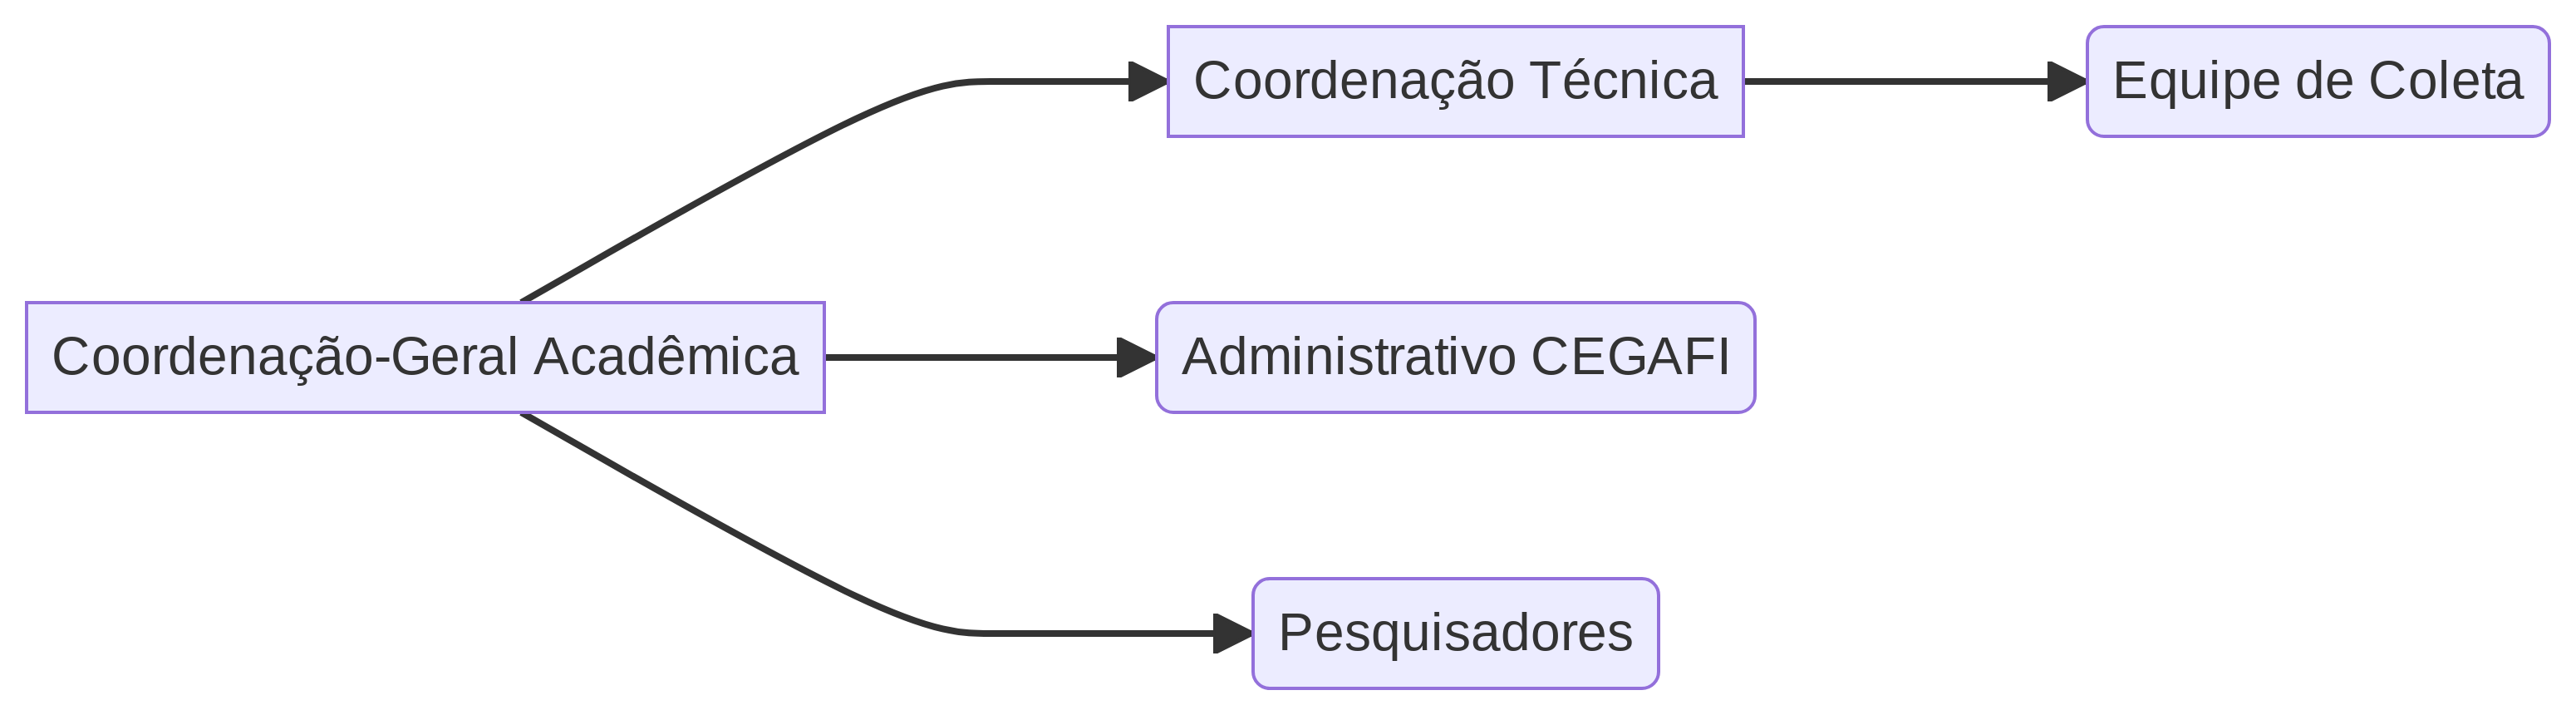
\includegraphics[width=8.07in,height=2.24in]{./3-metodologia_files/figure-latex/mermaid-figure-1.png}

}

\end{figure}

O fluxo das informações deverá seguir impreterivelmente a hierarquia
apresentada acima.

\hypertarget{coordenauxe7uxe3o-geral-acaduxeamica}{%
\subsection{\texorpdfstring{\emph{Coordenação-Geral
Acadêmica:}}{Coordenação-Geral Acadêmica:}}\label{coordenauxe7uxe3o-geral-acaduxeamica}}

\begin{itemize}
\tightlist
\item
  Representa a universidade junto com a entidade parceira e possui
  relação institucional com o INCRA;
\item
  Gerencia as atuações da Coordenação-Técnica, Administrativo CEGAFI e
  Pesquisadores.
\end{itemize}

\hypertarget{coordenauxe7uxe3o-tuxe9cnica}{%
\subsection{\texorpdfstring{\emph{Coordenação-Técnica:}}{Coordenação-Técnica:}}\label{coordenauxe7uxe3o-tuxe9cnica}}

\begin{itemize}
\item
  Responsável pelo planejamento das ações de campo, acompanhamento da
  execução física;
\item
  Gerencia o fornecimento de informações para a Coordenação-Geral,
  CEGAFI e Pesquisadores;
\item
  Responsável pela relação técnica com o INCRA e pela elaboração dos
  relatórios técnicos.
\end{itemize}

\hypertarget{administrativo-cegafi}{%
\subsection{\texorpdfstring{\emph{Administrativo
CEGAFI:}}{Administrativo CEGAFI:}}\label{administrativo-cegafi}}

\begin{itemize}
\tightlist
\item
  Responsável pelas rotinas administrativas do projeto (Recursos
  Humanos, Fundação e outros);
\end{itemize}

\hypertarget{pesquisadores}{%
\subsection{\texorpdfstring{\emph{Pesquisadores:}}{Pesquisadores:}}\label{pesquisadores}}

\begin{itemize}
\tightlist
\item
  Responsável pelas análises de dados e produtos acadêmicos.
\end{itemize}

\hypertarget{equipe-de-coleta}{%
\subsection{\texorpdfstring{\emph{Equipe de
coleta:}}{Equipe de coleta:}}\label{equipe-de-coleta}}

\begin{itemize}
\tightlist
\item
  Responsável pela coleta de dados em campo.
\end{itemize}

\hypertarget{fluxo-de-funcionamento-das-coletas}{%
\section{Fluxo de Funcionamento das
Coletas}\label{fluxo-de-funcionamento-das-coletas}}

\begin{figure}[H]

{\centering 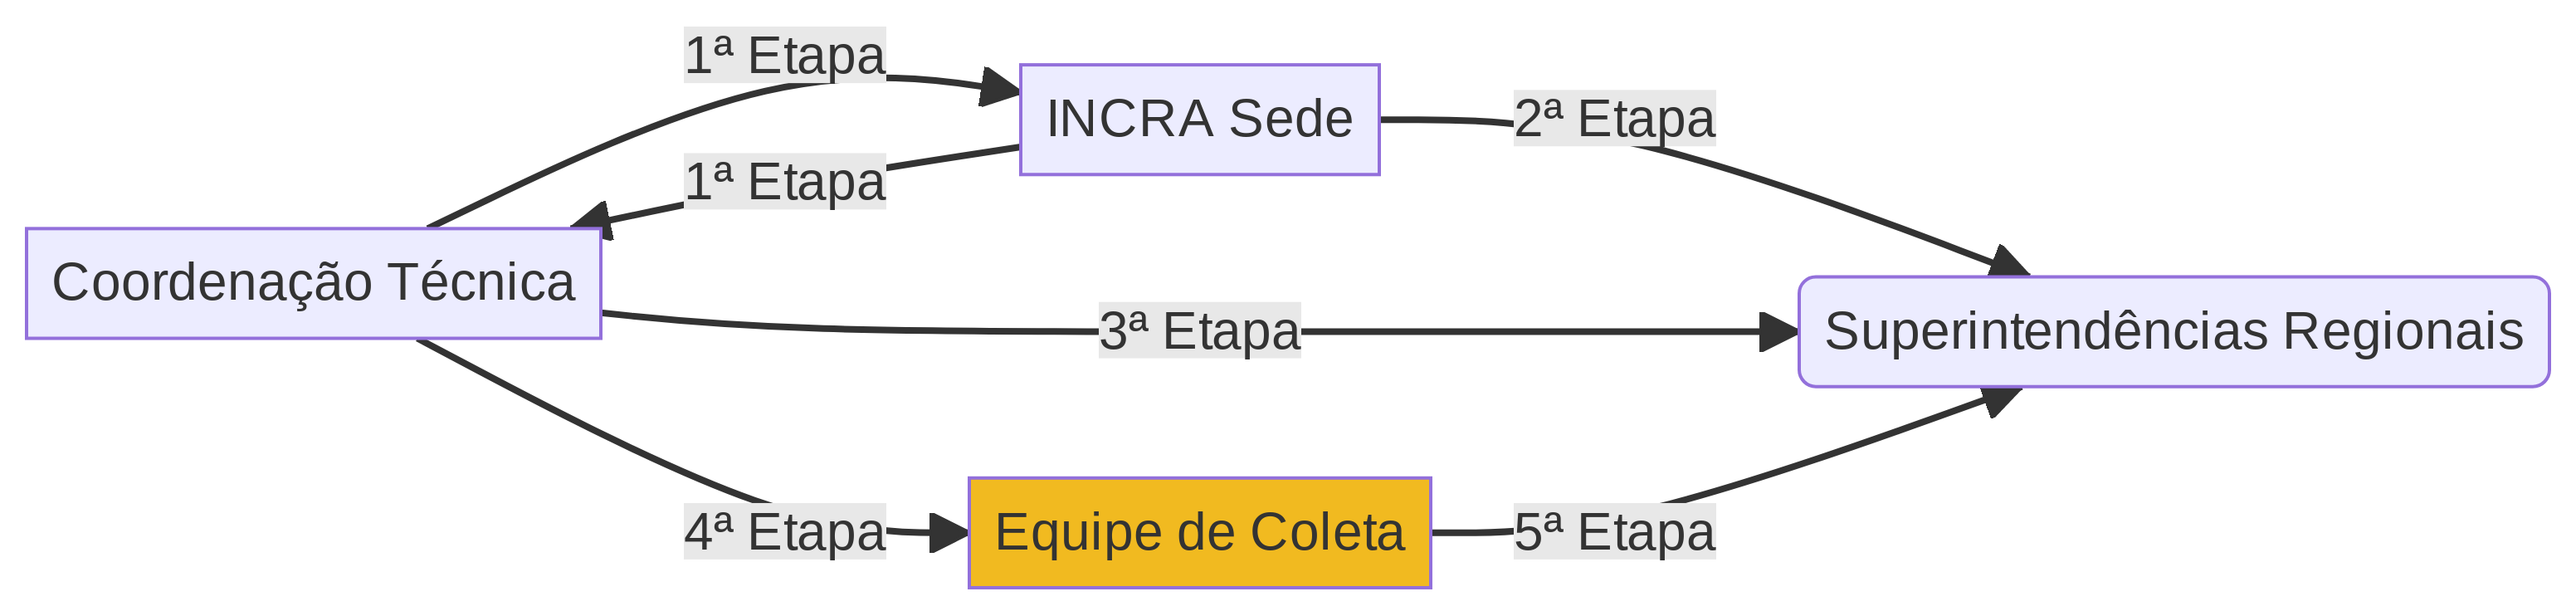
\includegraphics[width=8.08in,height=1.92in]{./3-metodologia_files/figure-latex/mermaid-figure-2.png}

}

\end{figure}

\textbf{1º etapa:} A coordenação Técnica pactua junto com Incra as
demandas e prioridades para o desenvolvimento do trabalho e solicita que
o Incra Sede informe a atuação dos trabalhos para Superintendência
Regional.

\textbf{2º etapa:} O Incra entra em contato com a Regional para informar
as demandas e prioridades.

\textbf{3º etapa:} A Coordenação Técnica entra em contato com a
Superintendência Regional com intuito de pactuar a atuação dos
trabalhos, ajustar sala, entre outros.

\textbf{4º etapa:} A Coordenação Técnica apresenta a atividade para a
Equipe de Coleta.

\textbf{5º etapa:} A Equipe é deslocada para Superintendência Regional
para executar a coleta de dados.

\bookmarksetup{startatroot}

\hypertarget{definiuxe7uxe3o-das-variuxe1veis-coletadas.}{%
\chapter{Definição das variáveis
coletadas.}\label{definiuxe7uxe3o-das-variuxe1veis-coletadas.}}

\hypertarget{informauxe7uxf5es-gerais.}{%
\section{Informações gerais.}\label{informauxe7uxf5es-gerais.}}

Com o intuito de padronizar o procedimento de coleta de dados e
levantamento das informações referente aos documentos titulatórios,
passamos a orientar os trabalhos com a finalidade de diminuir dúvidas e
facilitar a execução. É necessário observar algumas padronizações
gerais, são elas:

\begin{itemize}
\tightlist
\item
  Será obrigatório o preenchimento de todos os campos;
\item
  Quando não localizar a informação de qualquer campo, é necessário
  preencher com \textbf{``N/C''};
\item
  Todos os campos deverão ser preenchidos em \textbf{``CAIXA ALTA''}.
  \emph{\textbf{Ex: GLEBA XIRIRI''.}}
\item
  NÃO poderá preencher os campos com caracteres especiais;
\end{itemize}

\hypertarget{informauxe7uxe3o-sobre-os-imuxf3veis}{%
\section{Informação sobre os
imóveis}\label{informauxe7uxe3o-sobre-os-imuxf3veis}}

\hypertarget{identificauxe7uxe3o}{%
\subsection{\texorpdfstring{\emph{Identificação}}{Identificação}}\label{identificauxe7uxe3o}}

\emph{Nome do imóvel}

\begin{itemize}
\tightlist
\item
  Obrigatória;
\item
  Campo aberto;
\item
  Não aceita caracteres especiais; regex seria {[}a-zA-Zà-úÀ-Ú0-9{]} que
  representa uma letra qualquer que pode estar no intervalo de a-z ou,
  de A-Z, ou de à-ú, ou de À-Ú, ou um número que pode estar entre 0 ou
  9.;
\item
  Fonte de Coleta Primária: Processo do Imóvel;
\item
  Fonte de Coleta Secundária: Matrícula em Nome do Imóvel, Ato de
  Destinação ou Incorporação.
\end{itemize}

\emph{Tipologia}

\begin{itemize}
\tightlist
\item
  Obrigatória;
\item
  Selecionar uma Opção
\end{itemize}

\begin{longtable}[]{@{}l@{}}
\toprule()
Opções \\
\midrule()
\endhead
PC \\
PAR \\
Projeto de Assentamento Conjunto \\
PEC \\
PA \\
PF \\
PIC \\
Núcleo colonial \\
Registrada em nome do INCRA para fins de regularização fundiária \\
Registrada em nome da União para fins de regularização fundiária \\
Convênio \\
N/C \\
\bottomrule()
\end{longtable}

\begin{itemize}
\tightlist
\item
  Fonte de Coleta Primária: Ato de Destinação ou Incorporação;
\item
  Fonte de Coleta Secundária: Bases de Dados (SIPRA, SNCR, SRTT).
\end{itemize}

\emph{Unidade da Federação}

\begin{itemize}
\tightlist
\item
  Obrigatória;
\item
  Selecionar uma Opção
\end{itemize}

\begin{longtable}[]{@{}l@{}}
\toprule()
Opções \\
\midrule()
\endhead
Acre \\
Amapá \\
Amazonas \\
Maranhão \\
Mato Grosso \\
Pará \\
Rondônia \\
Roraima \\
Tocantins \\
\bottomrule()
\end{longtable}

\begin{itemize}
\tightlist
\item
  Fonte de Coleta Primária: IBGE;
\item
  Fonte de Coleta Secundária: Dialogar com Servidores do Setor de
  Cadastro da Superintendência Regional, Divisão de Obtenção, Divisão do
  Desenvolvimento. e Chefe de Divisão.
\end{itemize}

\emph{Município}

\begin{itemize}
\tightlist
\item
  Obrigatória;
\item
  Selecionar múltiplas opções;
\item
  Opções de resposta: A lista de municípios é carregada de acordo com a
  UF selecionada seguindo a listagem do IBGE.
\end{itemize}

\emph{Campos preenchidos automaticamente}

\begin{itemize}
\tightlist
\item
  De acordo com a UF selecionada:

  \begin{itemize}
  \tightlist
  \item
    Região
  \end{itemize}
\item
  De acordo com o município selecionado:

  \begin{itemize}
  \tightlist
  \item
    Código do IBGE;
  \item
    Módulo fiscal do município;
  \item
    Fracionamento mínimo;
  \item
    Faixa de fronteira;
  \item
    Superintendência Regional (Falta relação dos municípios do Pará que
    pertencem a cada superintendência);
  \item
    Unidade avançada
  \end{itemize}
\item
  Obs: Esses campos não são exibidos em tela durante a coleta;
\item
  Fonte de Coleta Primária: IBGE;
\item
  Fonte de Coleta Secundária: Dialogar com Servidores do Setor de
  Cadastro da Superintendência Regional, Divisão de Obtenção, Divisão do
  Desenvolvimento. e Chefe de Divisão.
\end{itemize}

\hypertarget{afetauxe7uxe3o-e-caracteruxedsticas-quanto-a-alienauxe7uxe3o}{%
\subsection{\texorpdfstring{\emph{Afetação e características quanto a
alienação}}{Afetação e características quanto a alienação}}\label{afetauxe7uxe3o-e-caracteruxedsticas-quanto-a-alienauxe7uxe3o}}

\emph{Possui afetação específica?}

\begin{itemize}
\tightlist
\item
  Selecionar uma opção;
\item
  Opções de resposta:

  \begin{itemize}
  \tightlist
  \item
    Sim;
  \item
    Não;
  \item
    N/C.
  \end{itemize}
\item
  Fonte de Coleta Primária: Processo do Imóvel;
\item
  Fonte de Coleta Secundária: Cruzamento de Banco de Dados do SIGEF.
\end{itemize}

\emph{Tipo de afetação}

\begin{itemize}
\tightlist
\item
  Selecionar uma opção
\item
  Opções de resposta:

  \begin{itemize}
  \tightlist
  \item
    Terra indígena;
  \item
    Terreno de marinha e acrescidos;
  \item
    Terrenos marginais, ilhas fluviais e lacustres;
  \item
    Várzeas federais;
  \item
    Unidades de conservação;
  \item
    Reservada à administração militar federal;
  \item
    Florestas Públicas nos termos da Lei 11.284 de 02/03/2006;
  \item
    Contém acessão ou benfeitoria federal;
  \item
    Ocupada por Comunidade Quilombola;
  \item
    Outra finalidade pública ou interesse social da União;
  \item
    N/C.
  \end{itemize}
\item
  Fonte de Coleta Primária: Cruzamento de Banco de Dados do SIGEF;
\item
  Fonte de Coleta Secundária: Processo do Imóvel, Atos ou Relatórios da
  Superintendência Regional;

  \begin{itemize}
  \tightlist
  \item
    OBS: Buscar dados dentro da Superintendência.
  \end{itemize}
\end{itemize}

\emph{Características quanto a alienação}

\begin{itemize}
\tightlist
\item
  Selecionar uma opção;
\item
  Opções de resposta:

  \begin{itemize}
  \tightlist
  \item
    Totalmente Alienável;
  \item
    Parcialmente Alienável;
  \item
    Inalienável;
  \item
    N/C;
  \end{itemize}
\item
  Fonte de Coleta Primária: Fazer uma análise do tipo de afetação e
  comparar com o tamanho da afetação da área.
\end{itemize}

\hypertarget{cuxf3digos-e-publicauxe7uxf5es}{%
\subsection{\texorpdfstring{\emph{Códigos e
publicações}}{Códigos e publicações}}\label{cuxf3digos-e-publicauxe7uxf5es}}

\emph{Código SIPRA}

\begin{itemize}
\tightlist
\item
  Campo aberto;
\item
  Não é permitido caracteres especiais exceto: / e ,
\item
  Fonte de Coleta Primária: Processo do Imóvel;
\item
  Fonte de Coleta Secundária: Matrícula do Imóvel, Bases de Dados (SNCR,
  SIPRA, SRTT), dialogar com Servidores do Setor de Cadastro da
  Superintendência Regional, Divisão de Obtenção, Divisão do
  Desenvolvimento. e Chefe de Divisão.
\end{itemize}

\emph{Ato de incorporação}

\begin{itemize}
\item
  Selecionar uma opção;
\item
  Opções de resposta:

  \begin{itemize}
  \tightlist
  \item
    Decreto;
  \item
    Portaria/Resolução;
  \item
    Concessão;
  \item
    Escritura de compra e venda;
  \item
    N/C.
  \end{itemize}
\item
  Fonte de Coleta Primária: Processo do Imóvel;
\item
  Fonte de Coleta Secundária: Pesquisa nos documentos disponíveis e em
  sites como:

  \begin{itemize}
  \tightlist
  \item
    \href{https://www.in.gov.br/servicos/diario-oficial-da-uniao}{Diário
    Oficial da Unuão}
  \item
    \href{https://www.camara.leg.br/legislacao}{Câmara Federal}
  \end{itemize}
\end{itemize}

\emph{Número do ato de incorporação}

\begin{itemize}
\tightlist
\item
  Campo aberto;
\item
  Livre.
\item
  Fonte de Coleta Primária: Ato de Incorporação;
\item
  Fonte de Coleta Secundária: Bases de Dados (SNCR, SIPRA, SRTT),
  dialogar com Servidores do Setor de Cadastro da Superintendência
  Regional, Divisão de Obtenção, Divisão do Desenvolvimento. e Chefe de
  Divisão.
\end{itemize}

\emph{Data do ato}

\begin{itemize}
\tightlist
\item
  Data no formato DD/MM/AAAA
\item
  Fonte de Coleta Primária: Ato de Incorporação;
\item
  Fonte de Coleta Secundária: Bases do Incra (SNCR, SIPRA, SRTT).
\end{itemize}

\emph{Área do ato de incorporação (Ha)}

\begin{itemize}
\tightlist
\item
  Inserção do valor com no máximo de quatro casas decimais;
\item
  Após a coleta sempre será exibido o valor informado com quatro casas
  decimais;
\item
  Separador de milhar: ponto;
\item
  Separador decimal: vírgula;
\item
  Fonte de Coleta Primária: Ato de Incorporação;
\item
  Fonte de Coleta Secundária: Pesquisas em sites, Bases de Dados (SIPRA,
  SNCR, SRTT), dialogar com Servidores do Setor de Cadastro da
  Superintendência Regional, Divisão de Obtenção, Divisão do
  Desenvolvimento. e Chefe de Divisão.
\end{itemize}

\emph{Forma de aquisição/obtenção}

\begin{itemize}
\tightlist
\item
  Selecionar uma opção
\item
  Opções de resposta
\end{itemize}

\begin{longtable}[]{@{}l@{}}
\toprule()
Opções \\
\midrule()
\endhead
Adjudicação \\
Arrecadação Sumária \\
Cessão \\
Cessão Gratuita \\
Compra \\
Confisco \\
Dação em Pagamento \\
Desafetação \\
Desapropriação \\
Doação \\
Esc. Pública de Doação \\
Herança Jacente \\
Incorporação \\
Reversão de Domínio \\
Sub-Júdice \\
Transf. INCRA/UNIÃO \\
Transf. UNIÃO/INCRA \\
Vacância \\
N/C \\
\bottomrule()
\end{longtable}

\begin{itemize}
\tightlist
\item
  Fonte de Coleta Primária: Processo do Imóvel
\item
  Fonte de Coleta Secundária: Ato de Incorporação, dialogar com
  Servidores do Setor de Cadastro da Superintendência Regional, Divisão
  de Obtenção, Divisão do Desenvolvimento. e Chefe de Divisão, Bases de
  Dados (SIPRA, SNCR, SRTT).
\end{itemize}

\emph{Ato de destinação}

\begin{itemize}
\tightlist
\item
  Selecionar uma opção;
\item
  Opções de resposta:

  \begin{itemize}
  \tightlist
  \item
    Decreto;
  \item
    Portaria;
  \item
    Resolução;
  \item
    N/C.
  \end{itemize}
\item
  Fonte de Coleta Primária: Processo do Imóvel
\item
  Fonte de Coleta Secundária: Ato de Incorporação, dialogar com o Chefe
  de Divisão na Superintendência Regional, dialogar com os servidores da
  Divisão de Obtenção, Divisão do Desenvolvimento Pesquisas em sites,
  Bases de Dados (SNCR, SIPRA, SRTT).
\end{itemize}

\emph{Tipo de destinação}

\begin{itemize}
\tightlist
\item
  Selecionar uma opção;
\item
  Opções de resposta:
\end{itemize}

\begin{longtable}[]{@{}l@{}}
\toprule()
opções \\
\midrule()
\endhead
Assentamento \\
Cadastro histórico \\
Colonização \\
Experimentação \\
Núcleo urbano \\
Quilombola \\
Reserva biológica \\
Reserva ecológica \\
Reserva Florestal \\
Reserva indígena \\
Reserva técnica \\
Sem destinação \\
Utilidade pública \\
N/C \\
Outros \\
\bottomrule()
\end{longtable}

\emph{Qual}

\begin{itemize}
\tightlist
\item
  Campo aberto;
\item
  Questão condicional, caso responda ``Outros'' no item anterior.
\item
  Fonte de Coleta Primária: Processo do Imóvel;
\item
  Fonte de Coleta Secundária: Ato de Destinação.
\end{itemize}

\emph{Área do imóvel destinado (Ha)}

\begin{itemize}
\tightlist
\item
  Inserção do valor com no máximo de quatro casas decimais;
\item
  Após a coleta sempre será exibido o valor informado com quatro casas
  decimais;
\item
  Separador de milhar: ponto;
\item
  Separador decimal: vírgula;
\item
  Fonte de Coleta Primária: Processo do Imóvel,
\item
  Fonte de Coleta Secundária: Plantas, Memorial Descritivo, Setor de
  Cartografia.
\end{itemize}

\hypertarget{matruxedcula}{%
\subsection{\texorpdfstring{\emph{Matrícula}}{Matrícula}}\label{matruxedcula}}

\emph{Número}

\begin{itemize}
\tightlist
\item
  Campo aberto;
\item
  Sem formatação.
\item
  Fonte de Coleta Primária: Processo do Imóvel;
\item
  Fonte de Coleta Secundária: Bases de Dados (SNCR, SIPRA,SRTT),
  dialogar com Servidores do Setor de Cadastro da Superintendência
  Regional, Divisão de Obtenção, Divisão do Desenvolvimento. e Chefe de
  Divisão.
\end{itemize}

\emph{Área (ha)}

\begin{itemize}
\tightlist
\item
  Inserção do valor com no máximo de quatro casas decimais;
\item
  Após a coleta sempre será exibido o valor informado com quatro casas
  decimais;
\item
  Separador de milhar: ponto;
\item
  Separador decimal: vírgula;
\item
  Fonte de Coleta Primária: Processo do Imóvel;
\item
  Fonte de Coleta Secundária: Plantas, Memorial Descritivo, Setor de
  Cartografia, Relatório das Divisões.
\end{itemize}

\emph{Data}

\begin{itemize}
\tightlist
\item
  Data no formato DD/MM/AAAA
\item
  Fonte de Coleta Primária: Processo do Imóvel;
\item
  Fonte de Coleta Secundária: Bases de Dados (SNCR, SIPRA,SRTT),
  Relatório das Divisões.
\end{itemize}

\emph{Titular}

\begin{itemize}
\tightlist
\item
  Selecionar uma opção;
\item
  Opções de resposta:

  \begin{itemize}
  \tightlist
  \item
    INCRA;
  \item
    UNIÃO;
  \item
    N/C.
  \end{itemize}
\item
  Fonte de Coleta Primária: Processo do Imóvel;
\item
  Fonte de Coleta Secundária: Bases de Dados (SNCR, SIPRA,SRTT),
  Relatório das Divisões.
\end{itemize}

\emph{Comarca}

\begin{itemize}
\tightlist
\item
  Campo aberto;
\item
  Sem formatação.
\item
  Fonte de Coleta Primária: Processo do Imóvel;
\item
  Fonte de Coleta Secundária: Bases de Dados (SNCR, SIPRA,SRTT),
  Relatório das Divisões.
\end{itemize}

\hypertarget{capacidade-do-imuxf3vel}{%
\subsection{\texorpdfstring{\emph{Capacidade do
imóvel}}{Capacidade do imóvel}}\label{capacidade-do-imuxf3vel}}

\emph{Número de parcelas urbanas}

\begin{itemize}
\tightlist
\item
  Campo aberto;
\item
  Somente números.
\item
  Fonte de Coleta Primária: Processo do Imóvel;
\item
  Fonte de Coleta Secundária: Bases de Dados (SNCR, SIPRA,SRTT),
  Relatório das Divisões.
\end{itemize}

\emph{Número de parcelas rurais}

\begin{itemize}
\tightlist
\item
  Campo aberto;
\item
  Somente números.
\item
  Fonte de Coleta Primária: Processo do Imóvel;
\item
  Fonte de Coleta Secundária: Bases de Dados (SNCR, SIPRA,SRTT),
  Relatório das Divisões.
\end{itemize}

\hypertarget{cartografia}{%
\subsection{\texorpdfstring{\emph{Cartografia}}{Cartografia}}\label{cartografia}}

\emph{Perímetro georreferenciado}

\begin{itemize}
\tightlist
\item
  Selecionar uma opção;
\item
  Opções de resposta:

  \begin{itemize}
  \tightlist
  \item
    Sim;
  \item
    Não;
  \item
    N/C.
  \end{itemize}
\item
  Fonte de Coleta Primária: SIGEF;
\item
  Fonte de Coleta Secundária: Dialogar com o Setor de Cartografia.
\end{itemize}

\emph{Perímetro certificado}

\begin{itemize}
\tightlist
\item
  Selecionar uma opção;
\item
  Opções de resposta:

  \begin{itemize}
  \tightlist
  \item
    Sim;
  \item
    Não;
  \item
    N/C.
  \end{itemize}
\item
  Fonte de Coleta Primária: SIGEF;
\item
  Fonte de Coleta Secundária: Dialogar com o Setor de Cartografia.
\end{itemize}

\hypertarget{informauxe7uxe3o-das-destinauxe7uxf5es.}{%
\section{Informação das
Destinações.}\label{informauxe7uxe3o-das-destinauxe7uxf5es.}}

\hypertarget{informauxe7uxf5es-individuais-sobre-a-titulauxe7uxe3o}{%
\subsection{\texorpdfstring{\emph{Informações individuais sobre a
titulação}}{Informações individuais sobre a titulação}}\label{informauxe7uxf5es-individuais-sobre-a-titulauxe7uxe3o}}

\emph{Número do processo}

\begin{itemize}
\tightlist
\item
  Campo obrigatório;
\item
  Campo aberto;
\item
  Fonte de Coleta Primária: Título de Domínio;
\item
  Fonte de Coleta Secundária: Anexos do Título, tais como: Planta,
  Memorial Descritivo, Certidão de Liberação de Cláusula, Certidão de
  Quitação, Certidão de Inteiro Teor do Imóvel.
\end{itemize}

\emph{Incluso no SEI?}

\begin{itemize}
\tightlist
\item
  Selecionar uma opção;
\item
  Opções de resposta:

  \begin{itemize}
  \tightlist
  \item
    Sim;
  \item
    Não;
  \item
    N/C.
  \end{itemize}
\item
  Fonte de Coleta Primária: Título de Domínio;
\item
  Fonte de Coleta Secundária: Anexos do Título, tais como: Planta,
  Memorial Descritivo, Certidão de Liberação de Cláusula, Certidão de
  Quitação, Certidão de Inteiro Teor do Imóvel.
\end{itemize}

\hypertarget{outorgado}{%
\subsection{\texorpdfstring{\emph{Outorgado}}{Outorgado}}\label{outorgado}}

\emph{Nome}

\begin{itemize}
\tightlist
\item
  Campo obrigatório;
\item
  Campo aberto;
\item
  Não é permitido caracteres especiais;
\item
  Fonte de Coleta Primária: Título de Domínio;
\item
  Fonte de Coleta Secundária: Anexos do Título, tais como: Planta,
  Memorial Descritivo, Certidão de Liberação de Cláusula, Certidão de
  Quitação, Certidão de Inteiro Teor do Imóvel.
\end{itemize}

\emph{CPF/CNPJ}

\begin{itemize}
\tightlist
\item
  Campo obrigatório;
\item
  Campo aberto;
\item
  Limite mínimo e máximo de caracteres;
\item
  Fonte de Coleta Primária: Título de Domínio;
\item
  Fonte de Coleta Secundária: Anexos do Título, tais como: Planta,
  Memorial Descritivo, Certidão de Liberação de Cláusula, Certidão de
  Quitação, Certidão de Inteiro Teor do Imóvel.
\item
  OBS: Discutir sobre a necessidade de conversão.
\end{itemize}

\emph{Gênero}

\begin{itemize}
\tightlist
\item
  Selecionar uma opção;
\item
  Opções de resposta:

  \begin{itemize}
  \tightlist
  \item
    Masculino;
  \item
    Feminino;
  \item
    N/C
  \end{itemize}
\item
  Fonte de Coleta Primária: Título de Domínio;
\item
  Fonte de Coleta Secundária: Anexos do Título, tais como: Planta,
  Memorial Descritivo, Certidão de Liberação de Cláusula, Certidão de
  Quitação, Certidão de Inteiro Teor do Imóvel.
\end{itemize}

\hypertarget{cuxf4njuge}{%
\subsection{\texorpdfstring{\emph{Cônjuge}}{Cônjuge}}\label{cuxf4njuge}}

\emph{Nome}

\begin{itemize}
\tightlist
\item
  Campo obrigatório;
\item
  Campo aberto;
\item
  Não é permitido caracteres especiais;
\item
  Fonte de Coleta Primária: Título de Domínio;
\item
  Fonte de Coleta Secundária: Anexos do Título, tais como: Planta,
  Memorial Descritivo, Certidão de Liberação de Cláusula, Certidão de
  Quitação, Certidão de Inteiro Teor do Imóvel.
\end{itemize}

\emph{CPF}

\begin{itemize}
\tightlist
\item
  Campo obrigatório;
\item
  Campo aberto;
\item
  Limite mínimo e máximo de caracteres;
\item
  Fonte de Coleta Primária: Título de Domínio;
\item
  Fonte de Coleta Secundária: Anexos do Título, tais como: Planta,
  Memorial Descritivo, Certidão de Liberação de Cláusula, Certidão de
  Quitação, Certidão de Inteiro Teor do Imóvel.
\end{itemize}

\emph{Gênero}

\begin{itemize}
\tightlist
\item
  Selecionar uma opção;
\item
  Opções de resposta:

  \begin{itemize}
  \tightlist
  \item
    Masculino;
  \item
    Feminino;
  \item
    N/C
  \end{itemize}
\item
  Fonte de Coleta Primária: Título de Domínio;
\item
  Fonte de Coleta Secundária: Anexos do Título, tais como: Planta,
  Memorial Descritivo, Certidão de Liberação de Cláusula, Certidão de
  Quitação, Certidão de Inteiro Teor do Imóvel.
\end{itemize}

\hypertarget{localizauxe7uxe3o}{%
\subsection{\texorpdfstring{\emph{Localização}}{Localização}}\label{localizauxe7uxe3o}}

\emph{Unidade da Federação}

\begin{itemize}
\tightlist
\item
  Campo obrigatório;
\item
  Selecionar uma opção;
\item
  Opções de resposta:

  \begin{itemize}
  \tightlist
  \item
    Acre;
  \item
    Amapá;
  \item
    Amazonas;
  \item
    Maranhão;
  \item
    Mato Grosso;
  \item
    Pará;
  \item
    Rondônia;
  \item
    Roraima;
  \item
    Tocantins;
  \end{itemize}
\item
  Fonte de Coleta Primária: Título de Domínio;
\item
  Fonte de Coleta Secundária: Anexos do Título, tais como: Planta,
  Memorial Descritivo, Certidão de Liberação de Cláusula, Certidão de
  Quitação, Certidão de Inteiro Teor do Imóvel.
\end{itemize}

\emph{Município}

\begin{itemize}
\tightlist
\item
  Campo obrigatório;
\item
  Selecionar múltiplas opções;
\item
  Opções de resposta:

  \begin{itemize}
  \tightlist
  \item
    A lista de municípios é carregada de acordo com a UF selecionada
    seguindo a listagem do IBGE;
  \end{itemize}
\item
  Fonte de Coleta Primária: Título de Domínio;
\item
  Fonte de Coleta Secundária: Anexos do Título, tais como: Planta,
  Memorial Descritivo, Certidão de Liberação de Cláusula, Certidão de
  Quitação, Certidão de Inteiro Teor do Imóvel.
\end{itemize}

\emph{Zona rural ou urbana}

\begin{itemize}
\tightlist
\item
  Campo obrigatório
\item
  Selecionar uma opção;
\item
  Opções de resposta:

  \begin{itemize}
  \tightlist
  \item
    Rural;
  \item
    Urbana.
  \end{itemize}
\item
  Fonte de Coleta Primária: Título de Domínio;
\item
  Fonte de Coleta Secundária: Anexos do Título, tais como: Planta,
  Memorial Descritivo, Certidão de Liberação de Cláusula, Certidão de
  Quitação, Certidão de Inteiro Teor do Imóvel.
\end{itemize}

\emph{Nome do imóvel}

\begin{itemize}
\tightlist
\item
  Campo obrigatório;
\item
  Selecionar uma opção;
\item
  Opções de resposta:

  \begin{itemize}
  \tightlist
  \item
    A partir da UF selecionada, é carregada uma lista com o nome de
    todos os imóveis já coletados daquela UF.
  \end{itemize}
\item
  Fonte de Coleta Primária: Título de Domínio;
\item
  Fonte de Coleta Secundária: Anexos do Título, tais como: Planta,
  Memorial Descritivo, Certidão de Liberação de Cláusula, Certidão de
  Quitação, Certidão de Inteiro Teor do Imóvel.
\end{itemize}

\emph{Nome do sítio}

\begin{itemize}
\tightlist
\item
  Campo aberto;
\item
  Fonte de Coleta Primária: Título de Domínio;
\item
  Fonte de Coleta Secundária: Anexos do Título, tais como: Planta,
  Memorial Descritivo, Certidão de Liberação de Cláusula, Certidão de
  Quitação, Certidão de Inteiro Teor do Imóvel.
\end{itemize}

\emph{Localização na gleba}

\begin{itemize}
\tightlist
\item
  Campo aberto;
\item
  Fonte de Coleta Primária: Título de Domínio;
\item
  Fonte de Coleta Secundária: Anexos do Título, tais como: Planta,
  Memorial Descritivo, Certidão de Liberação de Cláusula, Certidão de
  Quitação, Certidão de Inteiro Teor do Imóvel.
\end{itemize}

\emph{Lote}

\begin{itemize}
\tightlist
\item
  Campo aberto;
\item
  Fonte de Coleta Primária: Título de Domínio;
\item
  Fonte de Coleta Secundária: Anexos do Título, tais como: Planta,
  Memorial Descritivo, Certidão de Liberação de Cláusula, Certidão de
  Quitação, Certidão de Inteiro Teor do Imóvel.
\end{itemize}

\hypertarget{coordenadas}{%
\subsection{\texorpdfstring{\emph{Coordenadas}}{Coordenadas}}\label{coordenadas}}

\emph{Latitude}

\begin{itemize}
\tightlist
\item
  Campo aberto;
\item
  Fonte de Coleta Primária: Título de Domínio;
\item
  Fonte de Coleta Secundária: Anexos do Título, tais como: Planta,
  Memorial Descritivo, Certidão de Liberação de Cláusula, Certidão de
  Quitação, Certidão de Inteiro Teor do Imóvel.
\end{itemize}

\emph{Longitude}

\begin{itemize}
\tightlist
\item
  Campo aberto;
\item
  Fonte de Coleta Primária: Título de Domínio;
\item
  Fonte de Coleta Secundária: Anexos do Título, tais como: Planta,
  Memorial Descritivo, Certidão de Liberação de Cláusula, Certidão de
  Quitação, Certidão de Inteiro Teor do Imóvel.
\end{itemize}

\emph{Área}

\begin{itemize}
\tightlist
\item
  Inserção do valor com no máximo de quatro casas decimais;
\item
  Separador de milhar: ponto;
\item
  Separador decimal: vírgula;
\item
  Caso a destinação seja da zona rural:

  \begin{itemize}
  \tightlist
  \item
    A área inserida deve ser em Ha e ter até quatro casas decimais
  \end{itemize}
\item
  Caso a destinação seja da zona urbana:

  \begin{itemize}
  \tightlist
  \item
    A área inserida deve ser em m² e ter até duas casas decimais.
  \item
    Obs: Fazer a conversão quando necessário.
  \end{itemize}
\item
  Fonte de Coleta Primária: Título de Domínio;
\item
  Fonte de Coleta Secundária: Anexos do Título, tais como: Planta,
  Memorial Descritivo, Certidão de Liberação de Cláusula, Certidão de
  Quitação, Certidão de Inteiro Teor do Imóvel.
\end{itemize}

\hypertarget{tuxedtulo}{%
\subsection{\texorpdfstring{\emph{Título}}{Título}}\label{tuxedtulo}}

\emph{Número do título}

\begin{itemize}
\tightlist
\item
  Campo aberto;
\item
  Fonte de Coleta Primária: Título de Domínio;
\item
  Fonte de Coleta Secundária: Anexos do Título, tais como: Planta,
  Memorial Descritivo, Certidão de Liberação de Cláusula, Certidão de
  Quitação, Certidão de Inteiro Teor do Imóvel.
\end{itemize}

\emph{Ano de emissão}

\begin{itemize}
\tightlist
\item
  Campo aberto;
\item
  Fonte de Coleta Primária: Título de Domínio;
\item
  Fonte de Coleta Secundária: Anexos do Título, tais como: Planta,
  Memorial Descritivo, Certidão de Liberação de Cláusula, Certidão de
  Quitação, Certidão de Inteiro Teor do Imóvel.
\end{itemize}

\emph{Liberação da cláusula resolutiva}

\begin{itemize}
\tightlist
\item
  Selecionar uma opção;
\item
  Opções de resposta:

  \begin{itemize}
  \tightlist
  \item
    Sim;
  \item
    Não;
  \item
    N/C.
  \end{itemize}
\item
  Fonte de Coleta Primária: Título de Domínio;
\item
  Fonte de Coleta Secundária: Anexos do Título, tais como: Planta,
  Memorial Descritivo, Certidão de Liberação de Cláusula, Certidão de
  Quitação, Certidão de Inteiro Teor do Imóvel.
\end{itemize}

\emph{Informação do pagamento}

\begin{itemize}
\tightlist
\item
  Selecionar uma opção;
\item
  Opções de resposta:

  \begin{itemize}
  \tightlist
  \item
    Sim;
  \item
    Não;
  \item
    N/C.
  \end{itemize}
\item
  Fonte de Coleta Primária: Título de Domínio;
\item
  Fonte de Coleta Secundária: Anexos do Título, tais como: Planta,
  Memorial Descritivo, Certidão de Liberação de Cláusula, Certidão de
  Quitação, Certidão de Inteiro Teor do Imóvel.
\end{itemize}

\emph{Situação do título}

\begin{itemize}
\tightlist
\item
  Selecionar uma opção;
\item
  Opções de resposta:

  \begin{itemize}
  \tightlist
  \item
    Emitido e entregue;
  \item
    Emitido e não entregue;
  \item
    Cancelado;
  \item
    N/C
  \end{itemize}
\item
  Fonte de Coleta Primária: Título de Domínio;
\item
  Fonte de Coleta Secundária: Anexos do Título, tais como: Planta,
  Memorial Descritivo, Certidão de Liberação de Cláusula, Certidão de
  Quitação, Certidão de Inteiro Teor do Imóvel.
\end{itemize}

\emph{O título é registrado}

\begin{itemize}
\tightlist
\item
  Selecionar uma opção;
\item
  Opções de resposta:

  \begin{itemize}
  \tightlist
  \item
    Sim;
  \item
    Não;
  \item
    N/C.
  \end{itemize}
\item
  Fonte de Coleta Primária: Título de Domínio;
\item
  Fonte de Coleta Secundária: Anexos do Título, tais como: Planta,
  Memorial Descritivo, Certidão de Liberação de Cláusula, Certidão de
  Quitação, Certidão de Inteiro Teor do Imóvel.
\end{itemize}

\hypertarget{matruxedcula-1}{%
\subsection{\texorpdfstring{\emph{Matrícula}}{Matrícula}}\label{matruxedcula-1}}

\emph{Número da matrícula}

\begin{itemize}
\tightlist
\item
  Campo aberto;
\item
  Fonte de Coleta Primária: Título de Domínio;
\item
  Fonte de Coleta Secundária: Anexos do Título, tais como: Planta,
  Memorial Descritivo, Certidão de Liberação de Cláusula, Certidão de
  Quitação, Certidão de Inteiro Teor do Imóvel.
\end{itemize}

\emph{Número CNC do Cartório}

\begin{itemize}
\tightlist
\item
  Campo Obrigatório para o caso de existir matrícula;
\item
  Fonte: Listagem do CNJ.
\end{itemize}

\bookmarksetup{startatroot}

\hypertarget{delimitauxe7uxe3o-geogruxe1fica}{%
\chapter{Delimitação Geográfica}\label{delimitauxe7uxe3o-geogruxe1fica}}

Nos capiyulos a seguir faremos uma análise dos dados literais e
espaciais das Glebas Públicas Federais do INCRA dentro da Amazônia Legal
e do estado do Maranhão. A área de estudo contempla os limites da
Amazônia Legal incluindo-se todo o estado do Maranhão, mesmo a porção
que encontra-se fora da delimitação oficial da amazônia legal
(Figure~\ref{fig-area-estudo}).

\begin{figure}[H]

{\centering 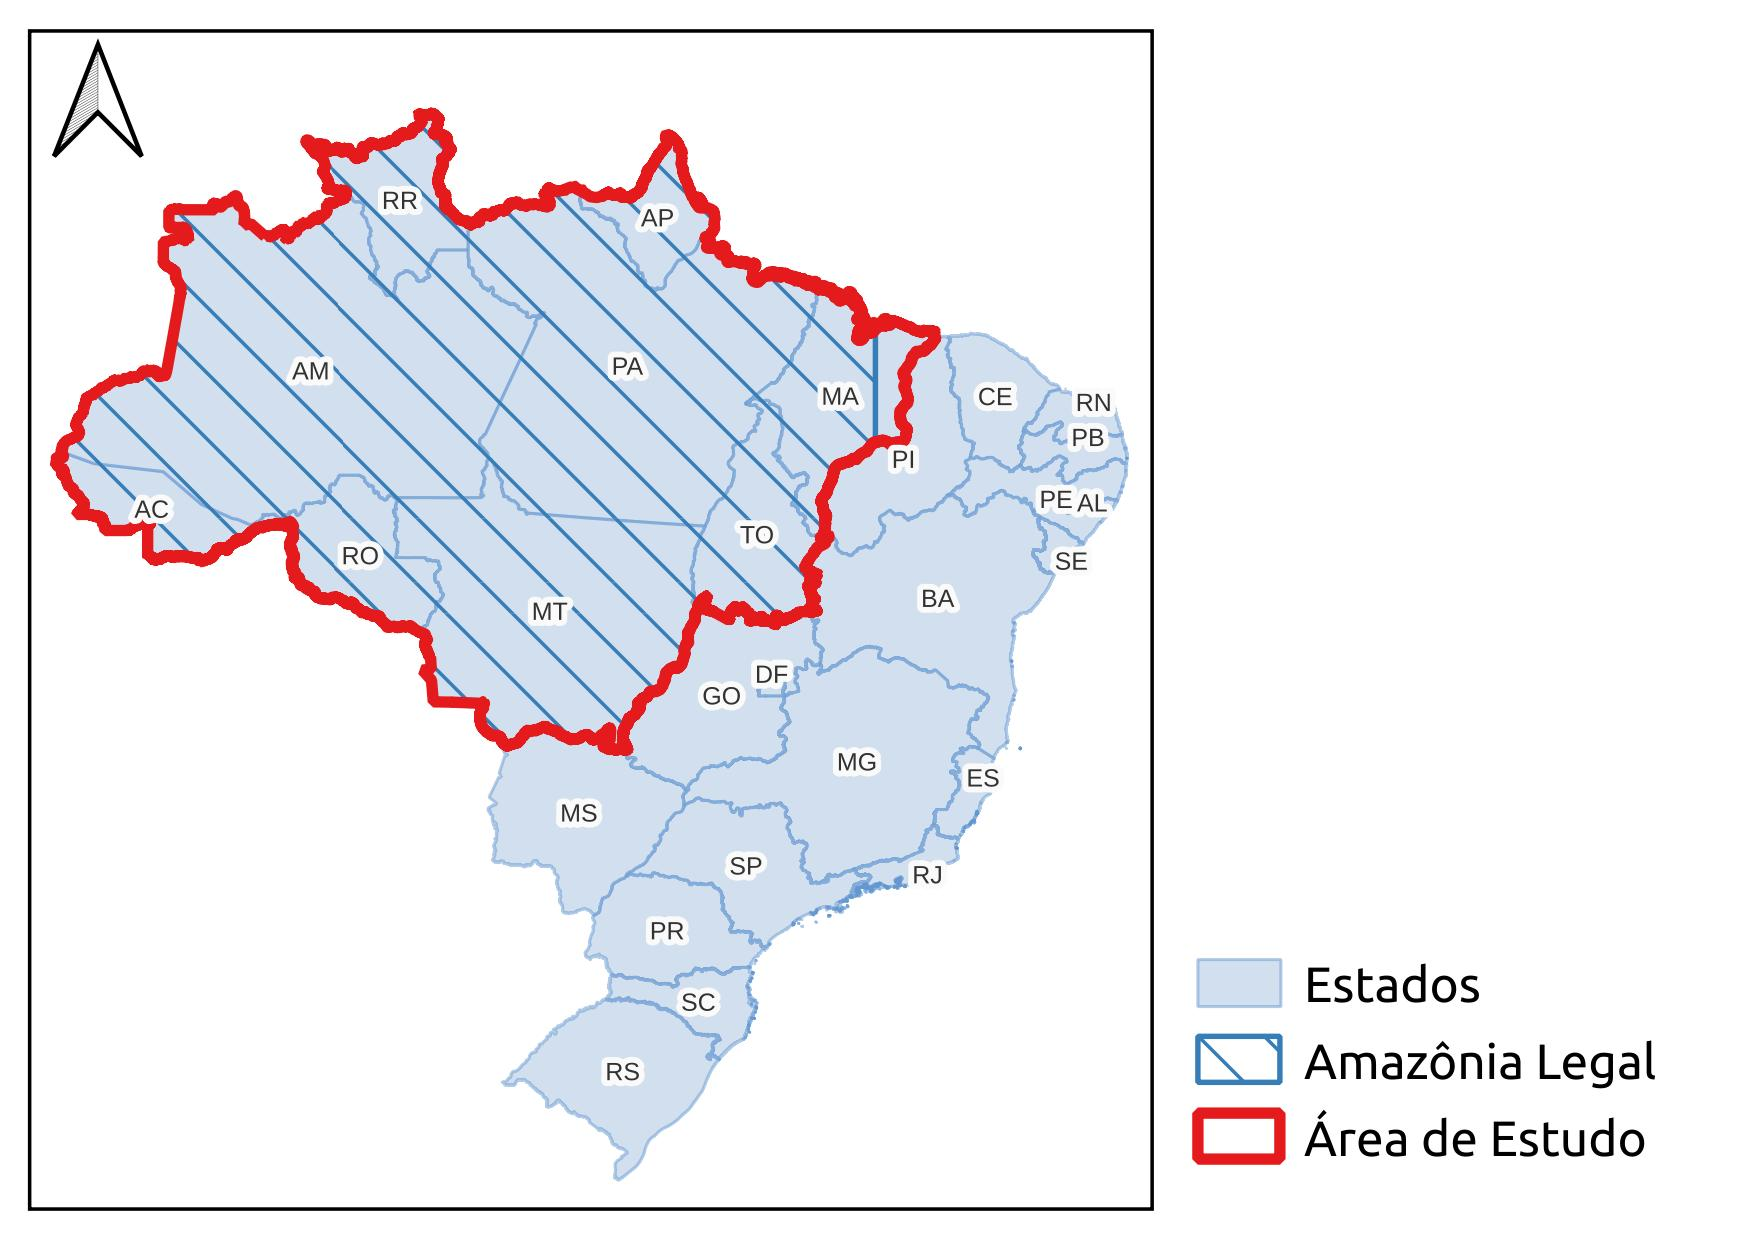
\includegraphics{././img/a6-geral.jpg}

}

\caption{\label{fig-area-estudo}Mapa de Área de Estudo}

\end{figure}

\hypertarget{mapa-das-glebas-puxfablicas-federais-dentro-da-uxe1rea-de-estudo.}{%
\section{Mapa das Glebas Públicas Federais dentro da área de
estudo.}\label{mapa-das-glebas-puxfablicas-federais-dentro-da-uxe1rea-de-estudo.}}

\includegraphics{./5-delimitacao_files/figure-pdf/cell-4-output-1.pdf}

\hypertarget{total-de-uxe1rea-das-gebas-federais-por-unidade-da-federauxe7uxe3o}{%
\section{Total de área das Gebas Federais por Unidade da
Federação}\label{total-de-uxe1rea-das-gebas-federais-por-unidade-da-federauxe7uxe3o}}

\n  

\n    

\n      

UF

\n      

Área (km²)

\n    

\n  

\n  

\n    

\n      

AC

\n      

15.563,3090

\n    

\n    

\n      

AM

\n      

387.961,0552

\n    

\n    

\n      

AP

\n      

48.644,4545

\n    

\n    

\n      

MA

\n      

32.497,7408

\n    

\n    

\n      

MT

\n      

79.546,5842

\n    

\n    

\n      

PA

\n      

372.493,7720

\n    

\n    

\n      

RO

\n      

163.572,2673

\n    

\n    

\n      

RR

\n      

4.994,1232

\n    

\n    

\n      

TO

\n      

55.653,6272

\n    

\n  

\n

\emph{1km² = 100ha}

\hypertarget{mapa-de-glebas-federais-por-unidade-da-federauxe7uxe3o.}{%
\section{Mapa de glebas federais por unidade da
federação.}\label{mapa-de-glebas-federais-por-unidade-da-federauxe7uxe3o.}}

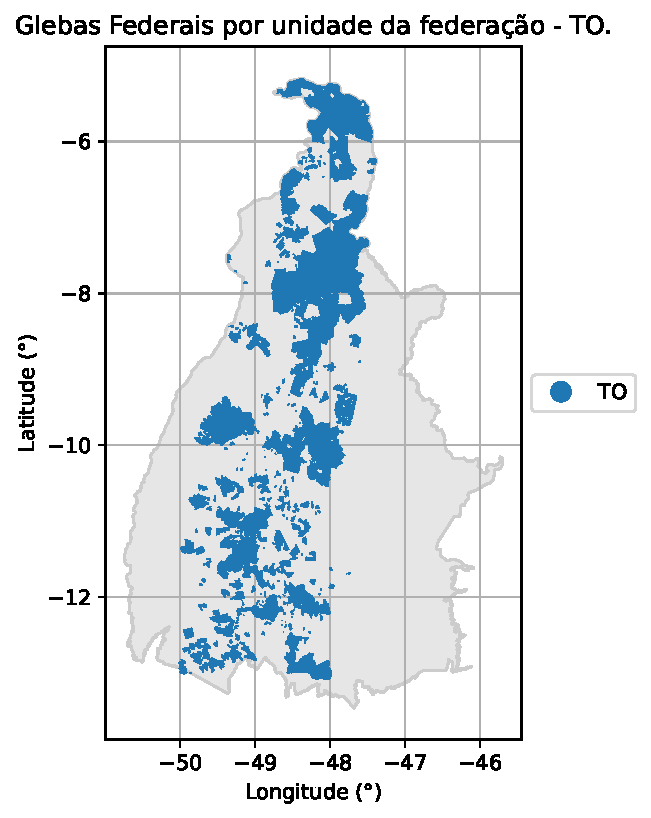
\includegraphics{./5-delimitacao_files/figure-pdf/cell-6-output-1.pdf}

\includegraphics{./5-delimitacao_files/figure-pdf/cell-6-output-2.pdf}

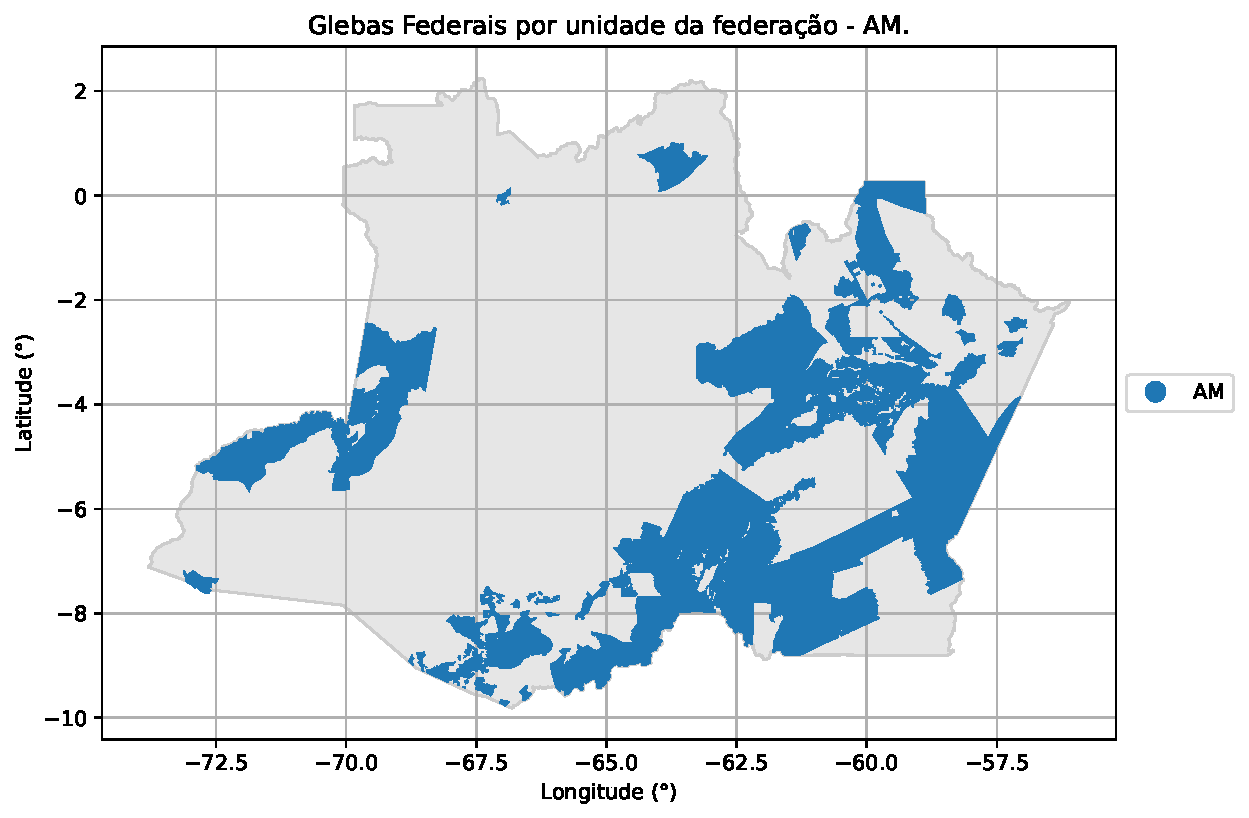
\includegraphics{./5-delimitacao_files/figure-pdf/cell-6-output-3.pdf}

\includegraphics{./5-delimitacao_files/figure-pdf/cell-6-output-4.pdf}

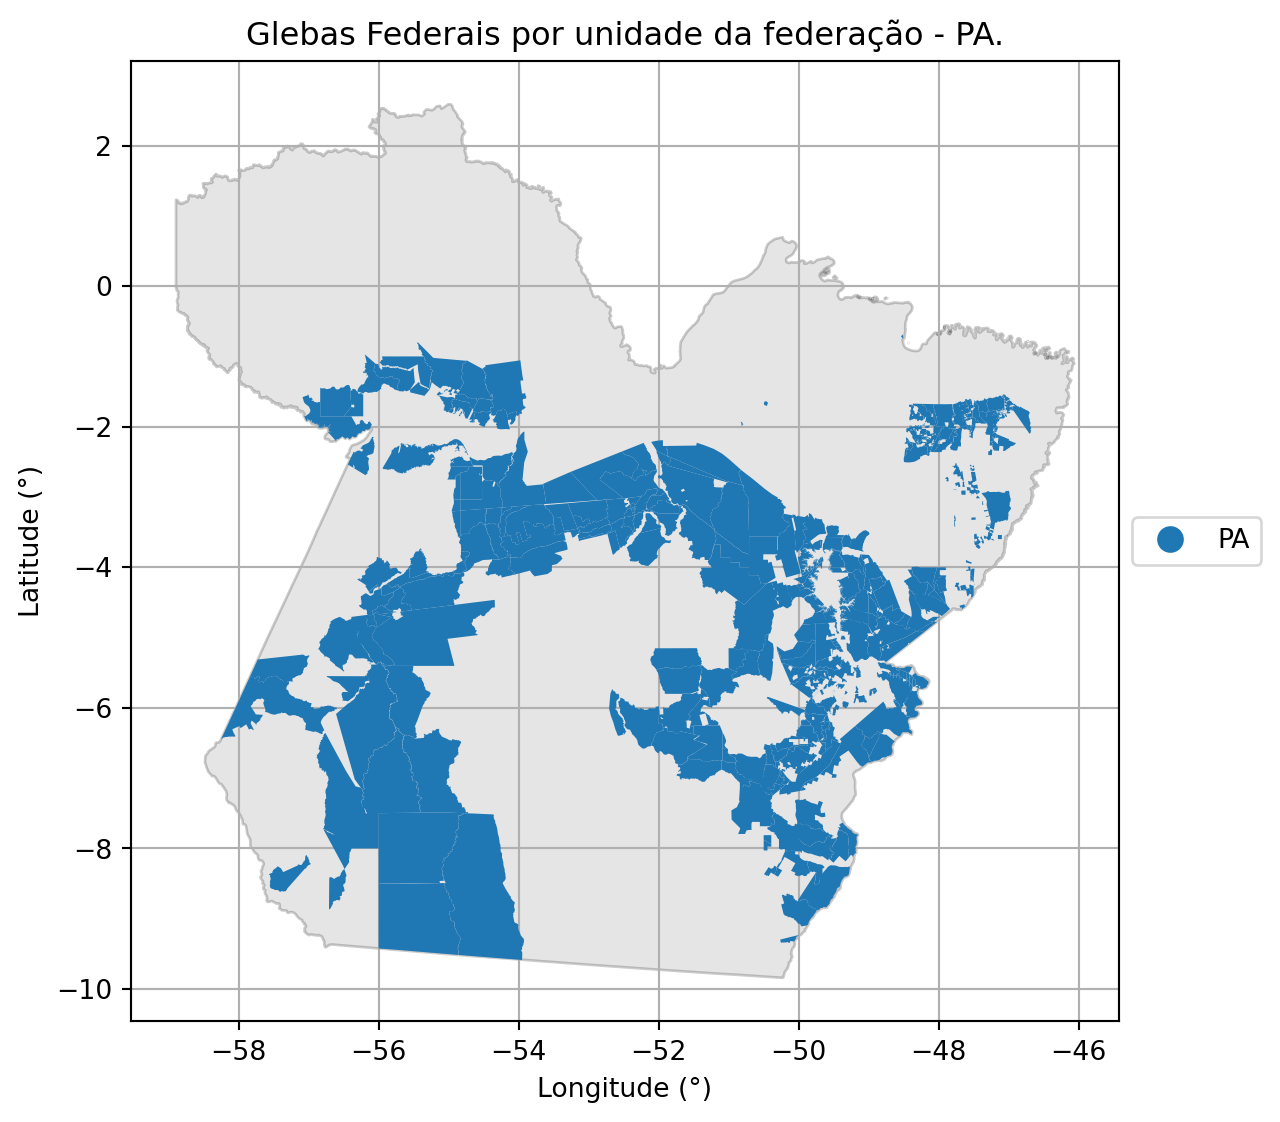
\includegraphics{./5-delimitacao_files/figure-pdf/cell-6-output-5.pdf}

\includegraphics{./5-delimitacao_files/figure-pdf/cell-6-output-6.pdf}

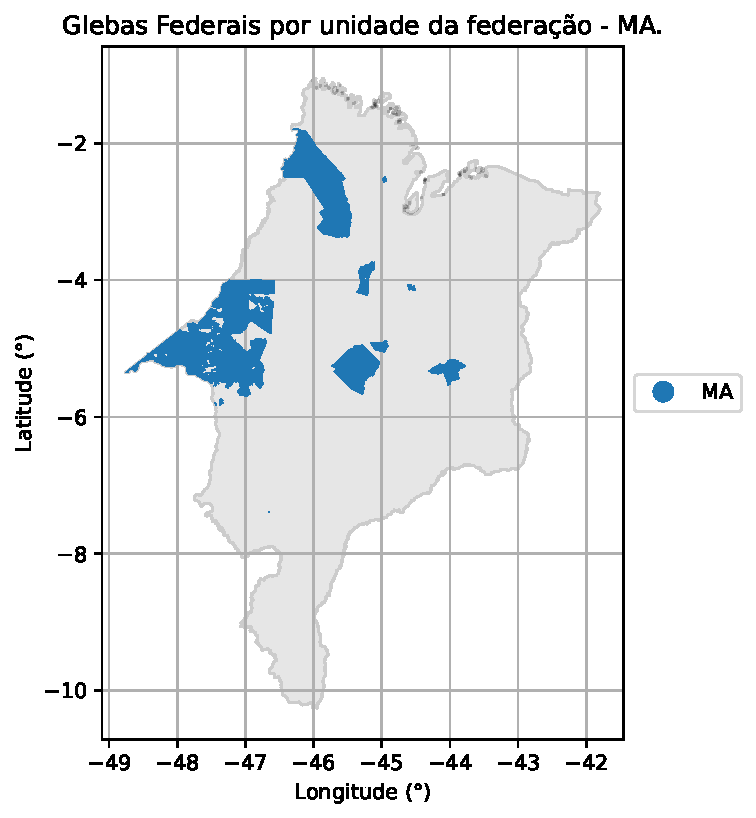
\includegraphics{./5-delimitacao_files/figure-pdf/cell-6-output-7.pdf}

\includegraphics{./5-delimitacao_files/figure-pdf/cell-6-output-8.pdf}

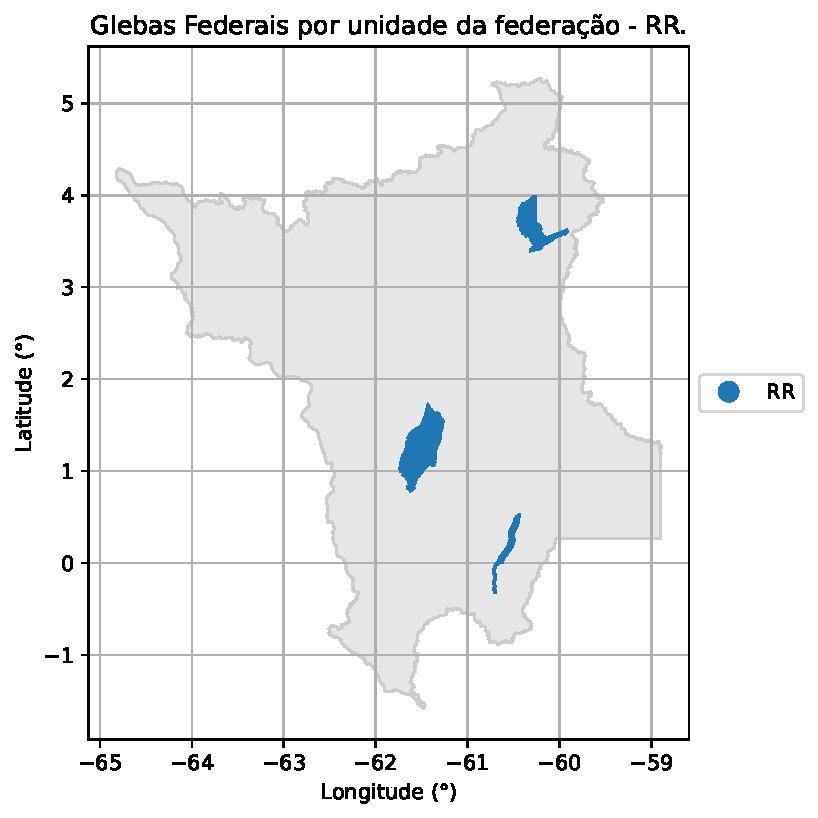
\includegraphics{./5-delimitacao_files/figure-pdf/cell-6-output-9.pdf}

\bookmarksetup{startatroot}

\hypertarget{detalhamento-das-informauxe7uxf5es-dos-atributos-relacionados-uxe0s-geometrias-das-glebas-federais.}{%
\chapter{Detalhamento das Informações dos atributos relacionados às
geometrias das Glebas
Federais.}\label{detalhamento-das-informauxe7uxf5es-dos-atributos-relacionados-uxe0s-geometrias-das-glebas-federais.}}

\begin{itemize}
\tightlist
\item
  \textbf{cod\_imovel} - código da gleba no Sistema Nacional de Cadastro
  Rural composto por 13 dígitos (000.000.000.000-0);
\item
  \textbf{matricula} - matrícula da gleba registrada em cartório,
  informação de texto com o número da matrícula, livro e cartório de
  registro;
\item
  \textbf{cartorio} - campo para armazenar o Código Nacional de
  Serventia do cartório de registro da gleba;
\item
  \textbf{nome\_gleba} - nome da gleba, informação de texto;
\item
  \textbf{nome\_comp} - coluna provisória para nomear as glebas sem
  denominação;
\item
  \textbf{sr} - superintendência responsável pela gleba;\\
\item
  \textbf{uf} - unidade da federação onde a gleba está localizada;\\
\item
  \textbf{situacao} - descrição não obtida. opções encontradas {[}null,
  Aprovação Fiscal, Arrecadada, Certificada, Registrada, Titulação{]};
\item
  \textbf{area\_ha} - área da gleba em hectares.
\item
  \textbf{data\_certi} - data da certificação da gleba.
\item
  \textbf{num\_certif} - código de certificação da gleba.
\item
  \textbf{status\_con} - aparenta ser a consulta da gleba na câmara
  técnica de regularização fundiária. opções {[}sem consulta,
  Consultada{]}, não está claro sobre o sentido da informação, se é
  aprovada ou não.
\item
  \textbf{assent\_pre} - assentimento prévio do Concelho de Defesa
  Nacional - CDN
\item
  \textbf{ano\_assent} - ano do assentimento
\item
  \textbf{data\_dou} - data de publicação no Diário Oficial da União
\item
  \textbf{ato} - descrição não obtida
\item
  \textbf{ciclo} - descrição não obtida
\item
  \textbf{documento} - descrição não obtida
\item
  \textbf{data\_doc} - descrição não obtida
\item
  \textbf{data\_encam} - descrição não obtida
\item
  \textbf{area\_sobre} - descrição não obtida
\item
  \textbf{gl\_fora\_am} - se a gleba está fora da amazônia legal
\item
  \textbf{ind\_area\_s} - descrição não obtida
\item
  \textbf{codigo\_gle} - descrição não obtida
\item
  \textbf{amaz\_legal} - se a área encontra-se dentro da área de estudo,
  1 para sim e 0 para não.
\item
  \textbf{lat} - latitude do centróide da poligonal
\item
  \textbf{lon} - longitude do centróide da poligonal
\item
  \textbf{geometry} - contém a geometria da gleba do tipo polígono.
\end{itemize}

\begin{center}\rule{0.5\linewidth}{0.5pt}\end{center}

\hypertarget{variuxe1veis-dentro-do-estudo-das-glebas-federais.}{%
\section{Variáveis dentro do estudo das Glebas
Federais.}\label{variuxe1veis-dentro-do-estudo-das-glebas-federais.}}

Para o prosseguimento do estudo, há uma necessidade de delimitação das
variáveis que irão compor a coleta de informações e como estas interagem
com outros temas sensíveis à delimitação e destinação das mesmas, seja
para áreas indígenas, unidades de conservação, assentamentos ou
regularização fundiária dos seus ocupantes. Isso requer informações que
orientem de forma racional dessa destinação.

\hypertarget{cuxf3digo-de-identificauxe7uxe3o-da-gleba-federal}{%
\subsection{Código de identificação da Gleba
Federal}\label{cuxf3digo-de-identificauxe7uxe3o-da-gleba-federal}}

De forma mais sensível ao cruzamento das glebas com os demais temas,
está sua identificação de forma única e inequívoca através de uma
codificação. Atualmente não há um sistema que identifique essas glebas,
muitas vezes tratadas por nomes locais que se repetem nas diferentes
regiões da Amazônia. Mesmo quando tratamos da mesma gleba, esta pode ser
composta de vários polígonos que recebem o mesmo nome, causando uma
ambiguidade nas análises espaciais e de fatores que podem ocorrer de
forma particular para cada polígono específico.

O Sistema de Gestão Fundiária (SIGEF) traz um código de certificação que
é dado a um polígono. Uma análise rápida de como o processo de
certificação ocorre, descarta o uso desta chave para identificação de
uma gleba ou parte dela, pelo fato do código da parcela certificada ser
mutável, ou seja, toda vez que um polígono é desmembrado ou dois
polígonos são remembrados, há a atribuição de novos códigos, podendo
gerar incongruência nas comparações de análises temporais de um gleba.

O Sistema de Cadastro Rural (SNCR) traz o código do imóvel rural, sendo
que o conceito de imóvel rural adotado pelo SNCR, atribui o mesmo código
a divérsos polígonos que podem compor um único imóvel rural. Esta
abordagem não resolve a identificação única de glebas com mais de um
polígono, os quais receberiam a mesma codificação.

Assim, com base na análise dos códigos já existentes e acima descritos,
o INCRA deve considerar a criação de um código único e inequívoco que
seja atribuído a cada polígono de uma gleba, sendo este imutável para a
área remanescente até que toda a gleba seja destinada e retirada do
patrimônio do INCRA, permitindo um balanço eficiente das áreas ainda sob
a tutela desta autarquia e permitindo cruzamentos de forma clara e
rápida com os outros temas abordados neste estudo e outros que venham a
surgir.

\hypertarget{matruxedcula-e-cuxf3digo-nacional-de-serventia-cns}{%
\subsection{Matrícula e Código Nacional de Serventia
(CNS)}\label{matruxedcula-e-cuxf3digo-nacional-de-serventia-cns}}

A informação registral das glabas é de suma importância no processo de
regularização fundiária e ajuda na identificação das glebas federais e
no seu regular desmembramento para um beneficiário, seja ele qual for.

As gelbas necessitam ter sua matrícula e o cartório no qual o registro
foi efetuado para que possamos sanar os procedimentos registrais das
áreas remanescentes e das já dentinadas, acompanhando o saldo
remanescente de cada matrídula.

\hypertarget{municuxedpio-e-unidade-da-federauxe7uxe3o}{%
\subsection{Município e Unidade da
Federação}\label{municuxedpio-e-unidade-da-federauxe7uxe3o}}

A localização das Glebas Federais em relação ao território municipal
onde estão localizadas e consequentimente ao estado da federação a que
pertencem causam confusão. As dimensões de algumas glebas e sua
localização nas fronteiras de entes federados acaba por gerar uma
disputa sobre seus recursos territoriais.

A certificação das peligonais atreladas ao correto registro cartorário
pode sanar este problema à medida que os polígonos respeitem os limites
político-administrativos e localizando cada porção da gleba no seu
município correspondente e comarca.

\hypertarget{situauxe7uxe3o}{%
\subsection{Situação}\label{situauxe7uxe3o}}

Esta variável apresenta-se amorfa, não sendo possível extrair qual seu
objetivo dentro das informações atribuídas à gleba. Atualmente as
informações consignadas nesta varíável são:

\begin{itemize}
\tightlist
\item
  Sem informações
\item
  Certificada
\item
  Arrecadada
\item
  Titulação
\item
  Registrada
\item
  Aprovação Fiscal
\end{itemize}

Faz-se necessário a definição do objetivo desta variável e a hierarquia
das informações consignadas na mesma, ou o desdobramento dos itens acima
relacionados em outras variáveis para que possam expressar a informação
de fase ou estado da gleba de forma clara.

\hypertarget{consulta-da-gleba-na-cuxe2mara-tuxe9cnica-de-destinauxe7uxe3o-e-regularizauxe7uxe3o-fundiuxe1ria-de-terras-puxfablicas-federais-rurais.}{%
\subsection{Consulta da gleba na Câmara Técnica de Destinação e
Regularização Fundiária de Terras Públicas Federais
Rurais.}\label{consulta-da-gleba-na-cuxe2mara-tuxe9cnica-de-destinauxe7uxe3o-e-regularizauxe7uxe3o-fundiuxe1ria-de-terras-puxfablicas-federais-rurais.}}

A informação disponpivel marca se a gelba foi consultada ou não, porém
não consta se foi aprovada para entrar no processo de regularização.
Outra informação que deve ser relacionada, seja como atributo nas
informações da gleba ou como uma outra camada espacial são as área que
foram requeridas ou interditadas por outros integrantes da câmara
(interesse concorrente).

\hypertarget{glebas-com-assentimento-pruxe9vio-do-concelho-de-defesa-nacional---cdn.}{%
\subsection{Glebas com assentimento prévio do Concelho de Defesa
Nacional -
CDN.}\label{glebas-com-assentimento-pruxe9vio-do-concelho-de-defesa-nacional---cdn.}}

Nesta variável está a informação das gelbas que necessitam de
assentimento prévio do Concelho de Defesa Nacional pois encontram-se na
faixa de 150 quilômetros da fronteira.

\hypertarget{geometria-da-gleba}{%
\subsection{Geometria da gleba}\label{geometria-da-gleba}}

As poligonais das glebas representam uma das informações mais
importantes para a sua administração. A certificação das glebas visa
estabelecer um perímetro que obedece a critérios tecnicos de precisão
cartográfica, possibilitando a sua correta localização, retificação e
ratificação registral, bem como a área real disponível para
regularização fundiária.

As glebas que não encontram-se certificadas necessitam de uma
verificação mínima nos polígonos que a representam para que possam ter
uma topologia válida, possibilitando cruzamentos espaciais com outras
entidades. Nas poligonais analizadas, foram encontradas uma série de
vértices sobrepostos e outros tipos de geometrias inválidas como
micropolígonos, ou polígonos com área zero, gerando inconsistências e
erros durante as análises espaciais.

\bookmarksetup{startatroot}

\hypertarget{cuxe2mara-tuxe9cnica-de-destinauxe7uxe3o-e-regularizauxe7uxe3o-fundiuxe1ria-de-terras-puxfablicas-federais-rurais.}{%
\chapter{Câmara Técnica de Destinação e Regularização Fundiária de
Terras Públicas Federais
Rurais.}\label{cuxe2mara-tuxe9cnica-de-destinauxe7uxe3o-e-regularizauxe7uxe3o-fundiuxe1ria-de-terras-puxfablicas-federais-rurais.}}

O Decreto nº 10.592, de 24 de dezembro de 2020, que Regulamenta a Lei nº
11.952, de 25 de junho de 2009, para dispor sobre a regularização
fundiária das áreas rurais situadas em terras da União, no âmbito da
Amazônia Legal, e em terras do Instituto Nacional de Colonização e
Reforma Agrária, por meio de alienação e concessão de direito real de
uso de imóveis, estabeleceu em ser Artigo 11° que:

\begin{quote}
Art. 11. Fica instituída a Câmara Técnica de Destinação e Regularização
Fundiária de Terras Públicas Federais Rurais, com as seguintes
finalidades:

I - atuar, de maneira articulada, na gestão do patrimônio público; e

II - convergir ações de destinação e promoção de políticas públicas.
\end{quote}

\begin{center}\rule{0.5\linewidth}{0.5pt}\end{center}

\hypertarget{distribuiuxe7uxe3o-de-glebas-federais-com-consulta-na-cuxe2mara-tuxe9cnica-de-destinauxe7uxe3o-e-regularizauxe7uxe3o-fundiuxe1ria-de-terras-puxfablicas-federais-rurais-por-unidade-da-federauxe7uxe3o.}{%
\section{Distribuição de Glebas Federais com consulta na Câmara Técnica
de Destinação e Regularização Fundiária de Terras Públicas Federais
Rurais por unidade da
federação.}\label{distribuiuxe7uxe3o-de-glebas-federais-com-consulta-na-cuxe2mara-tuxe9cnica-de-destinauxe7uxe3o-e-regularizauxe7uxe3o-fundiuxe1ria-de-terras-puxfablicas-federais-rurais-por-unidade-da-federauxe7uxe3o.}}

\includegraphics{./7-ctrf_files/figure-pdf/cell-4-output-1.pdf}

\hypertarget{glebas-federais-por-unidade-da-federauxe7uxe3o-com-consulta-na-cuxe2mara-tuxe9cnica-de-destinauxe7uxe3o-e-regularizauxe7uxe3o-fundiuxe1ria-de-terras-puxfablicas-federais-rurais.}{%
\section{Glebas Federais por unidade da federação com consulta na Câmara
Técnica de Destinação e Regularização Fundiária de Terras Públicas
Federais
Rurais.}\label{glebas-federais-por-unidade-da-federauxe7uxe3o-com-consulta-na-cuxe2mara-tuxe9cnica-de-destinauxe7uxe3o-e-regularizauxe7uxe3o-fundiuxe1ria-de-terras-puxfablicas-federais-rurais.}}

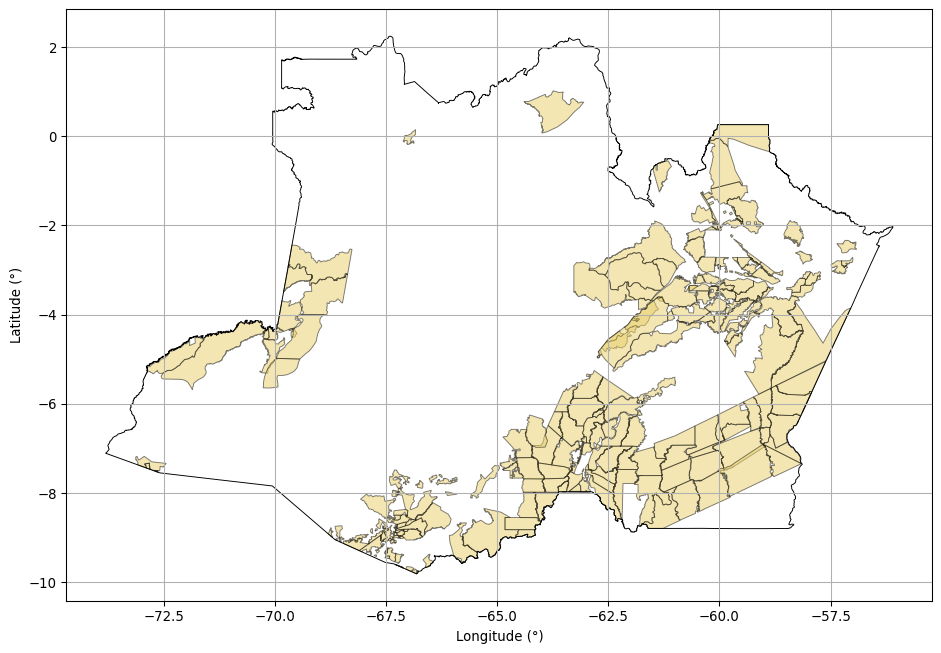
\includegraphics{./7-ctrf_files/figure-pdf/cell-5-output-1.pdf}

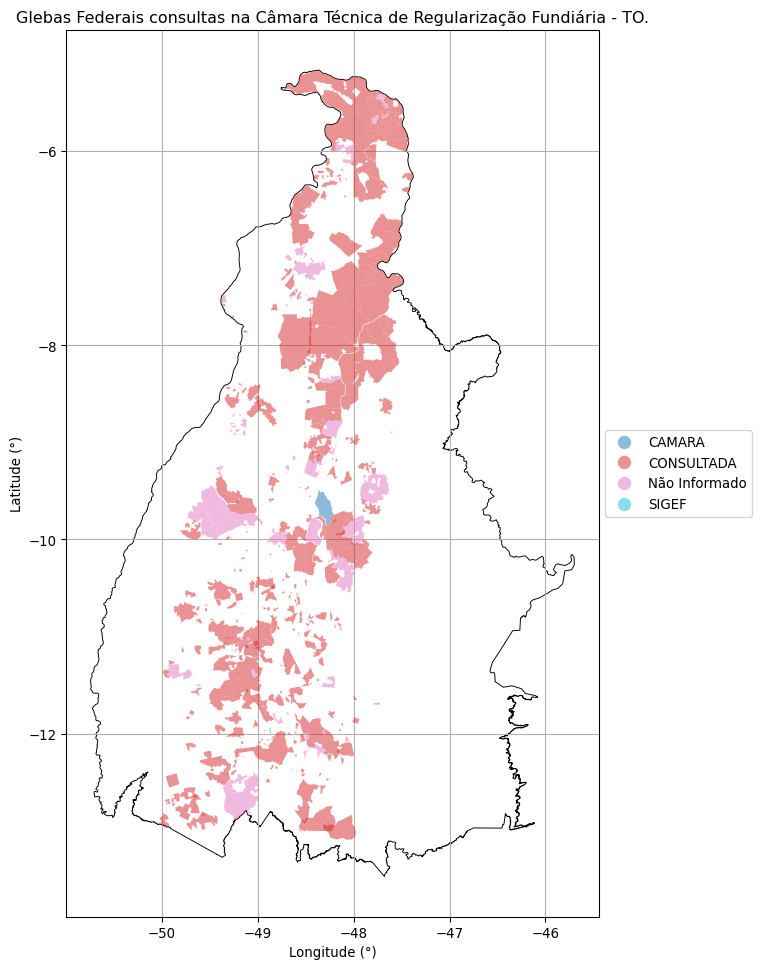
\includegraphics{./7-ctrf_files/figure-pdf/cell-5-output-2.pdf}

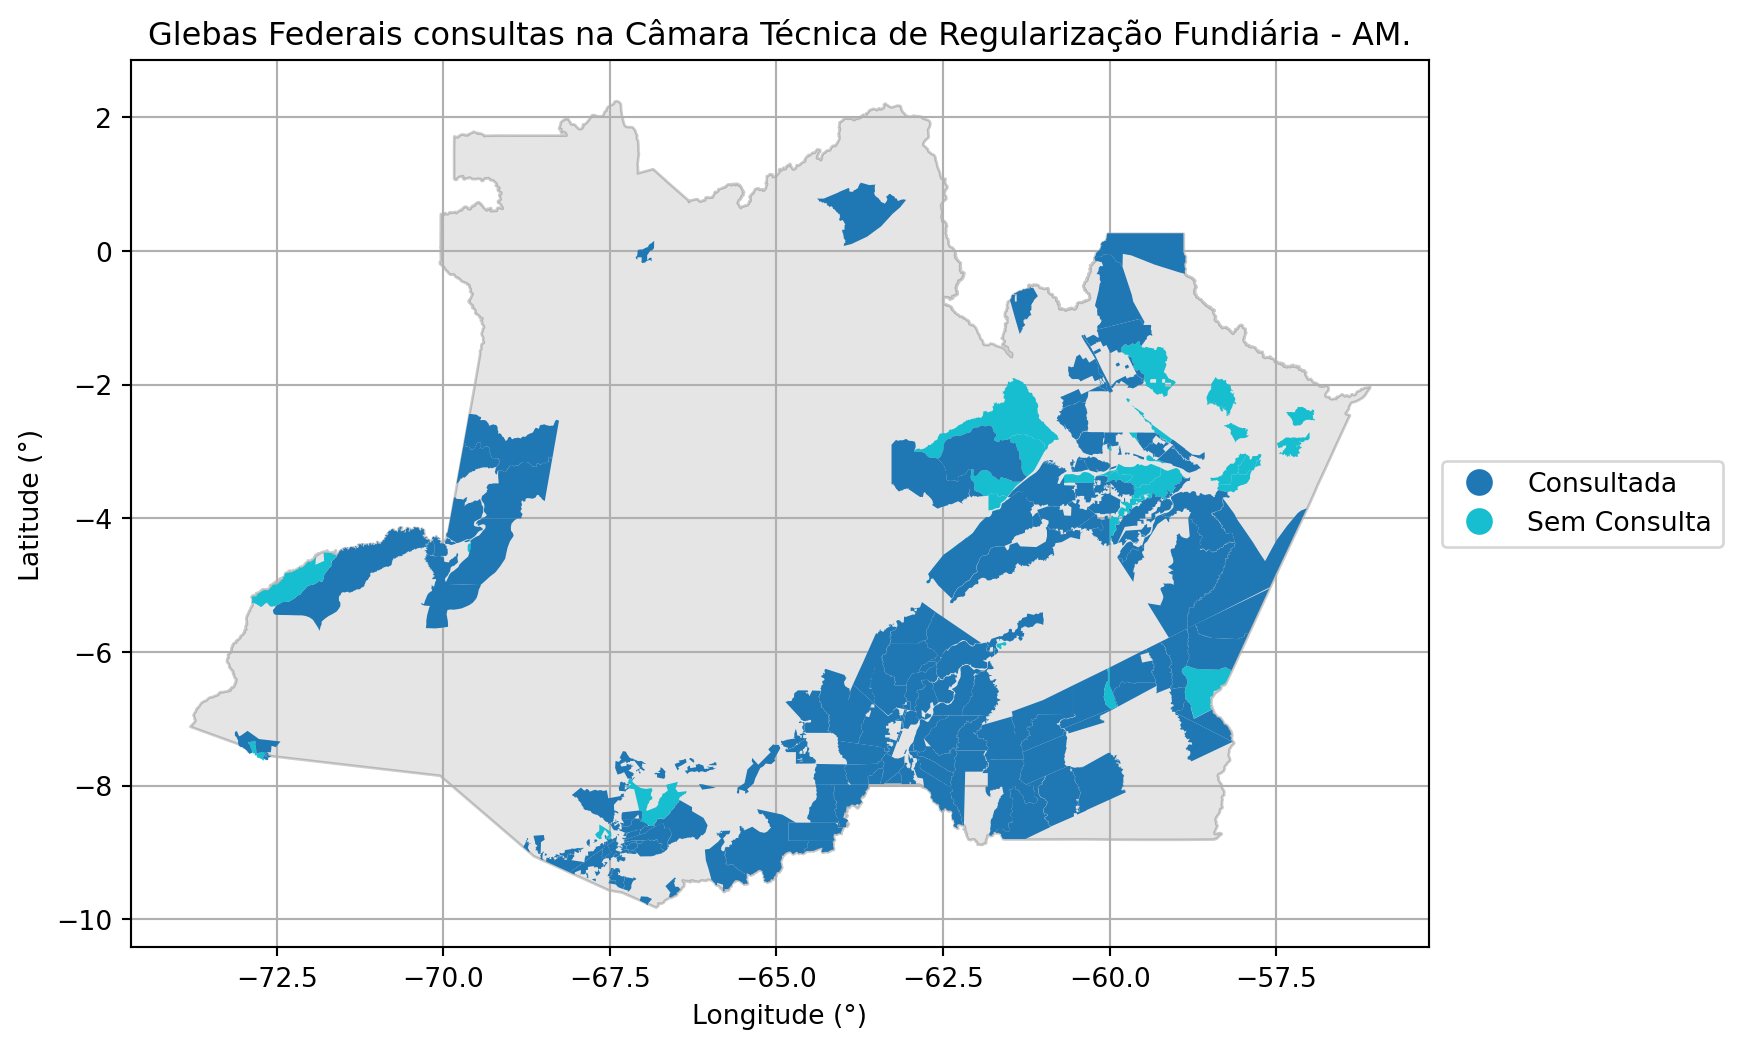
\includegraphics{./7-ctrf_files/figure-pdf/cell-5-output-3.pdf}

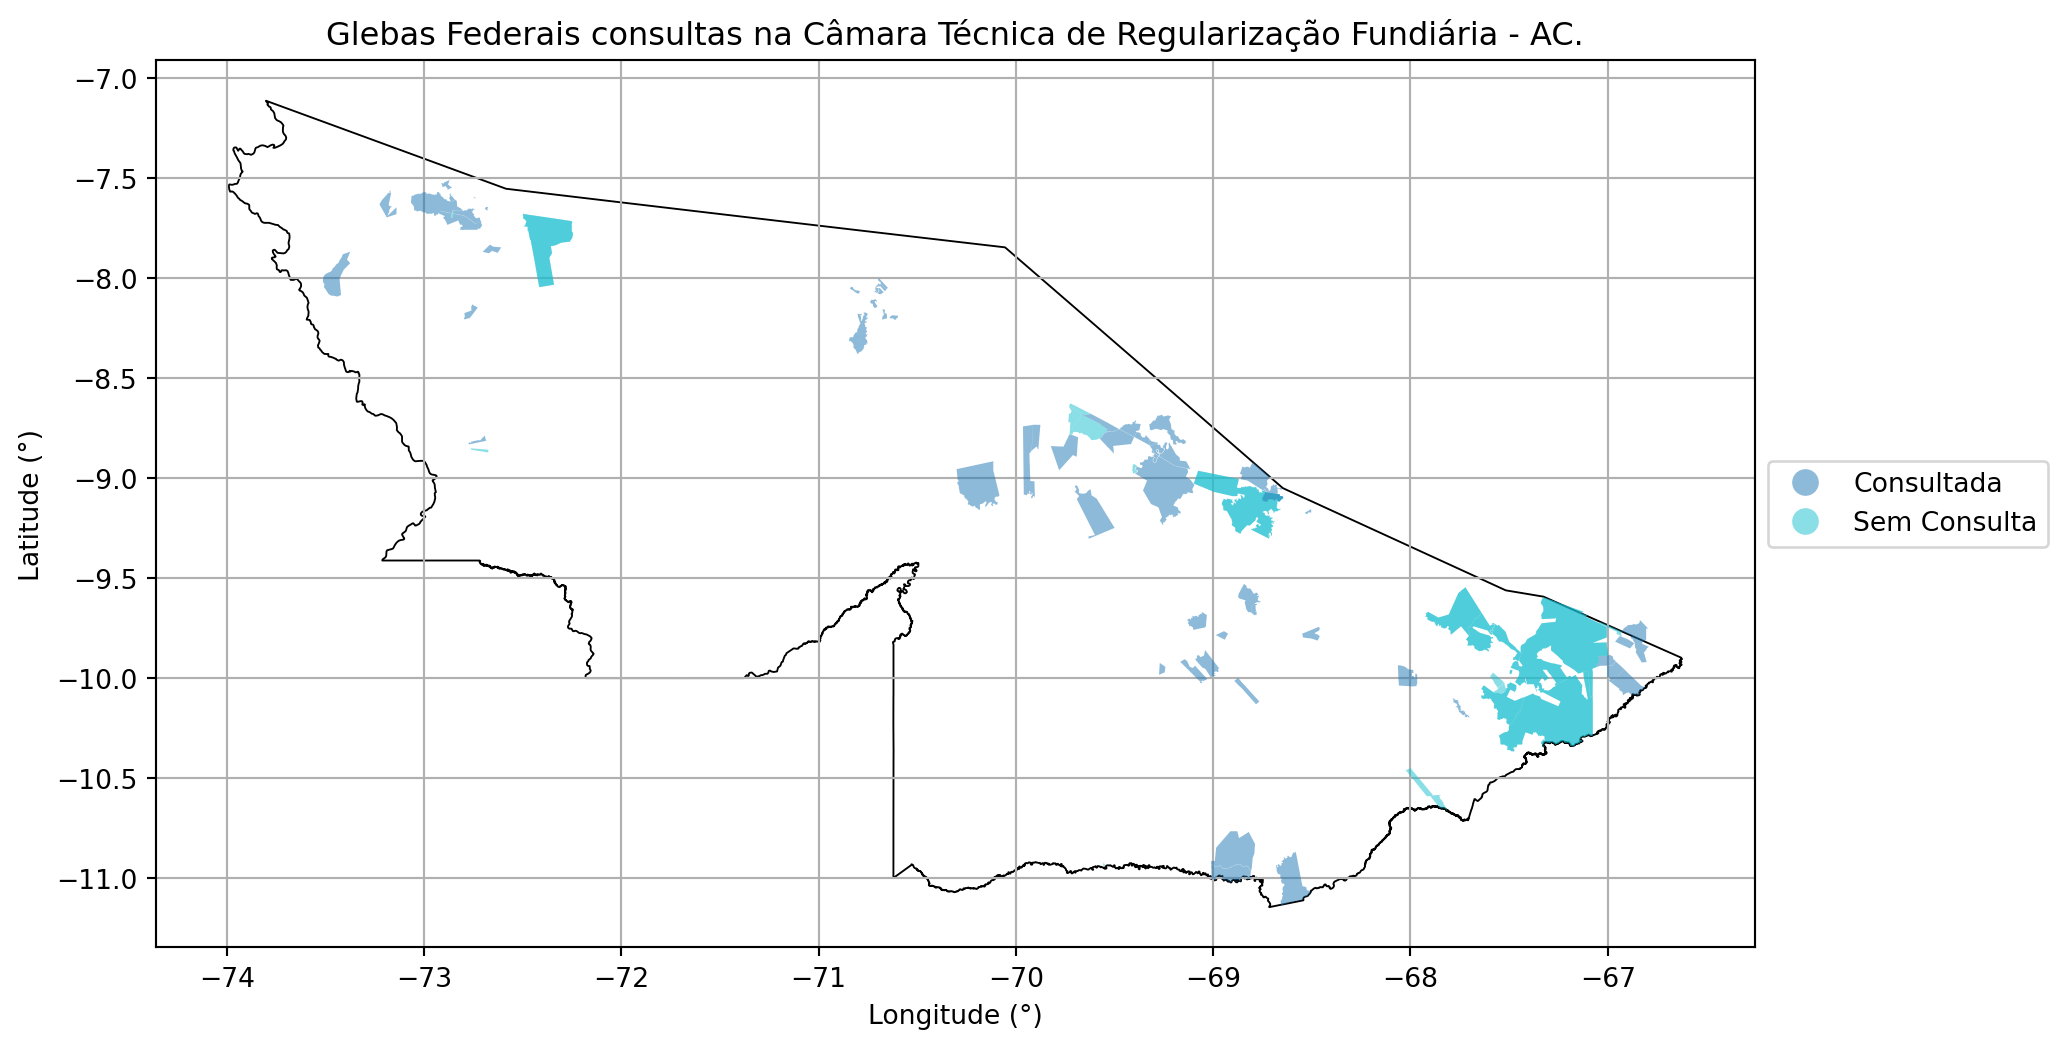
\includegraphics{./7-ctrf_files/figure-pdf/cell-5-output-4.pdf}

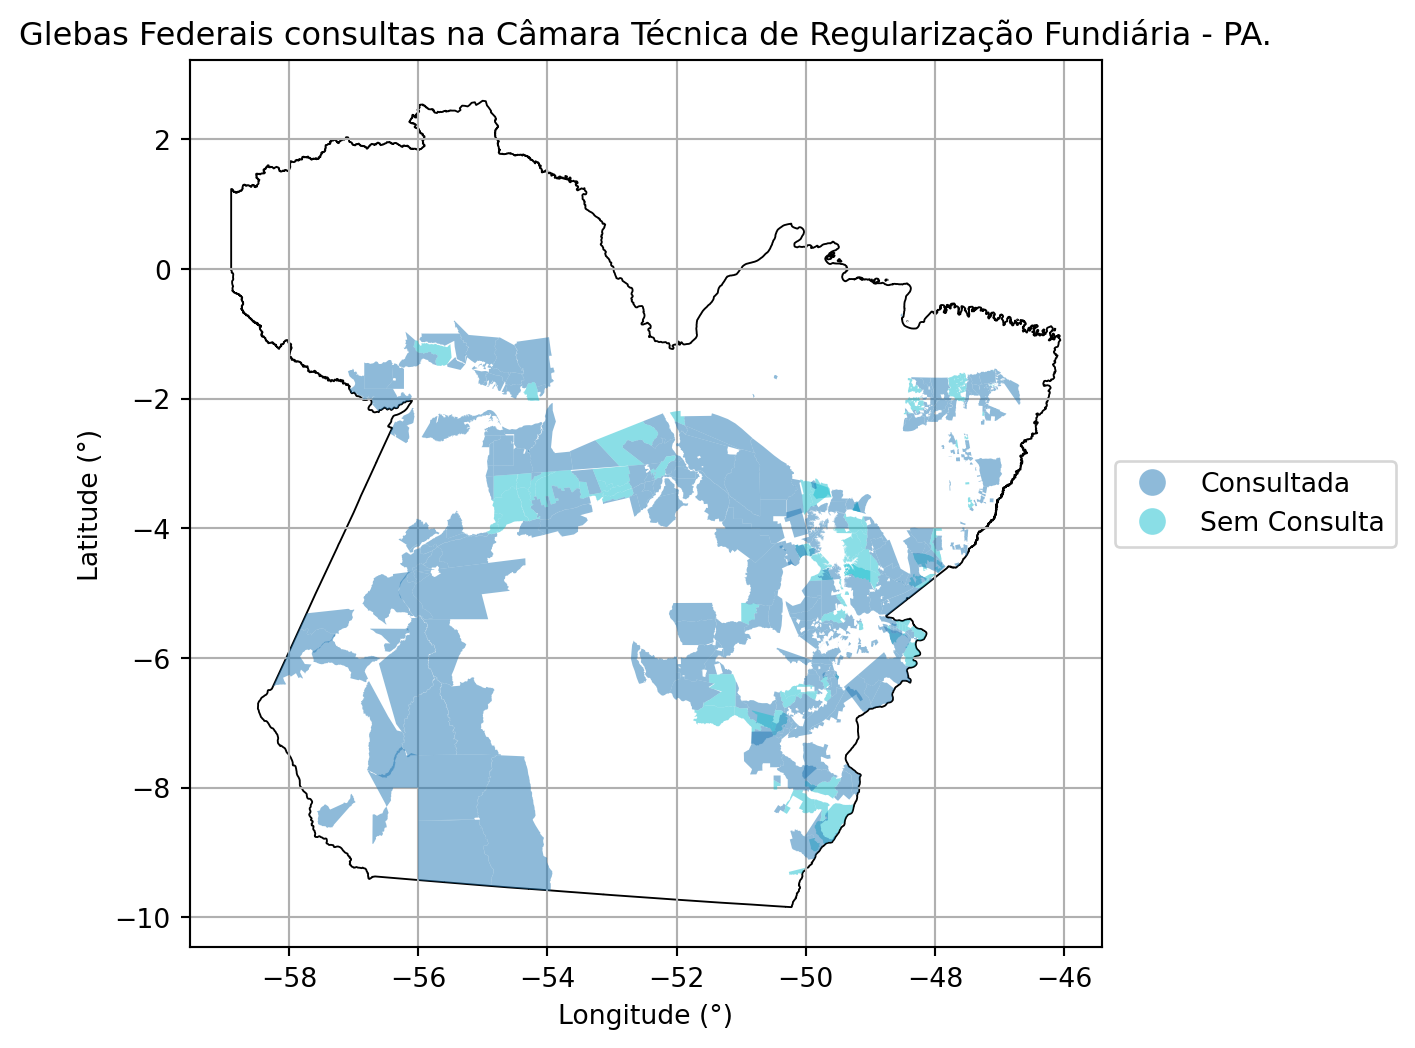
\includegraphics{./7-ctrf_files/figure-pdf/cell-5-output-5.pdf}

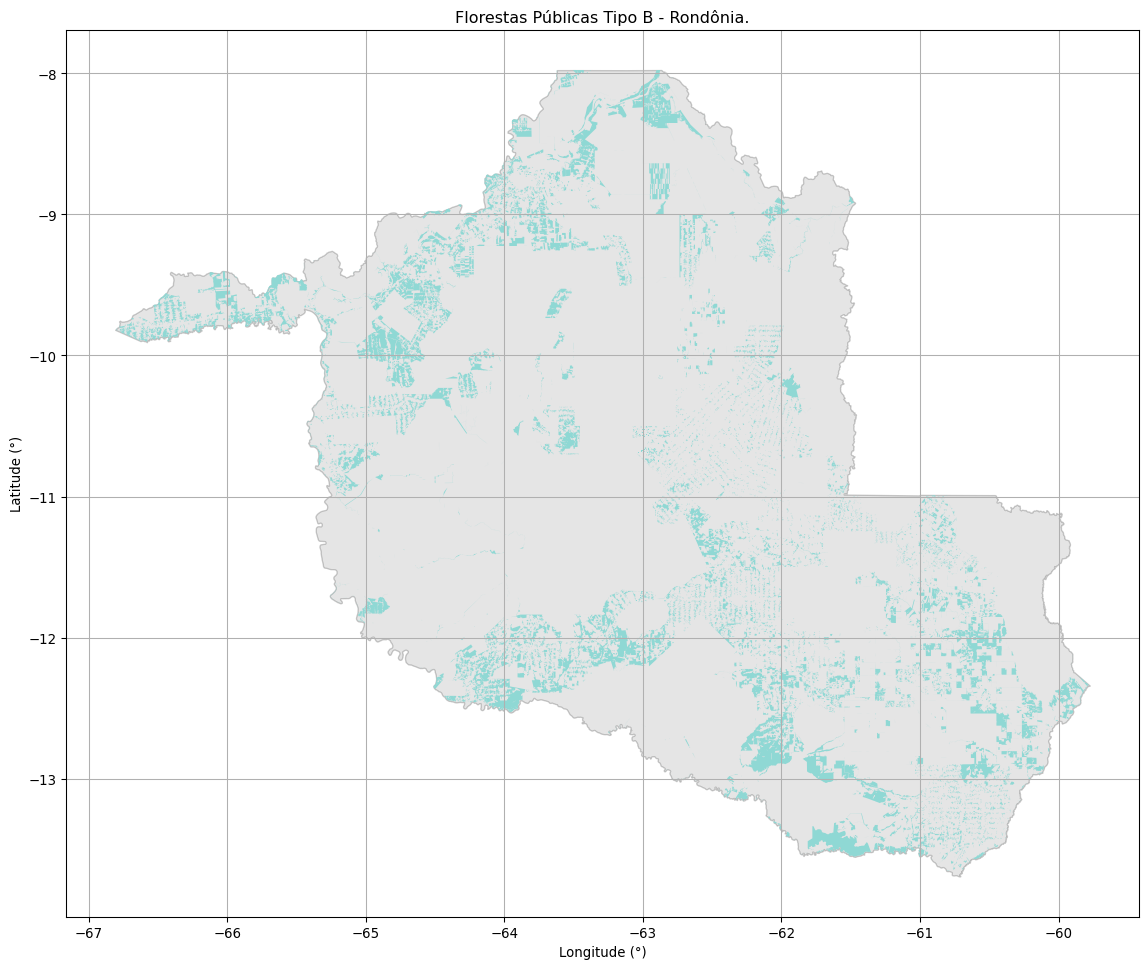
\includegraphics{./7-ctrf_files/figure-pdf/cell-5-output-6.pdf}

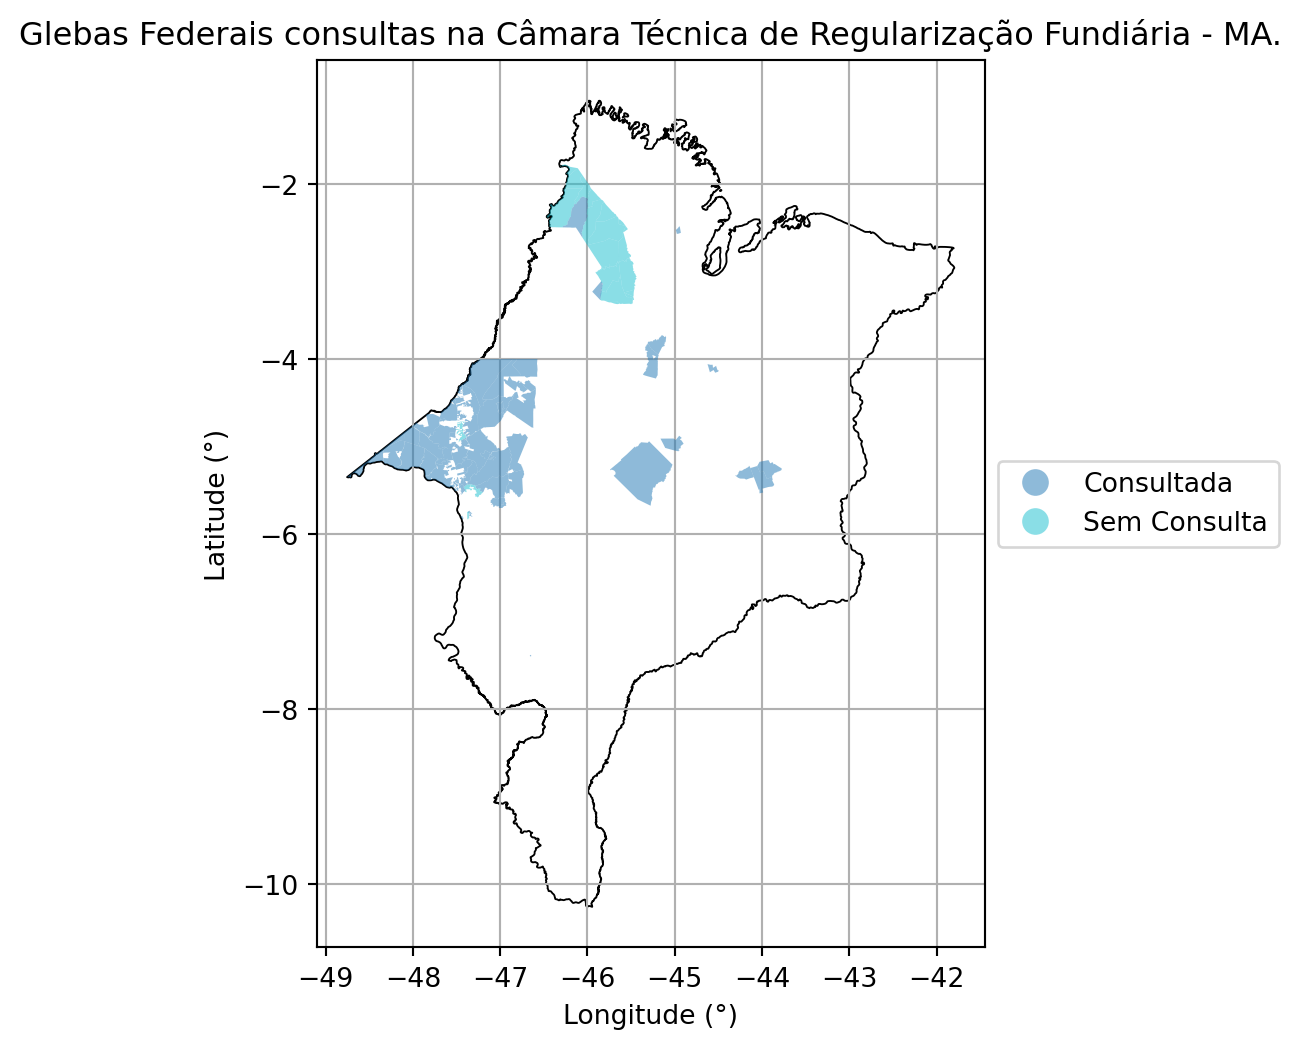
\includegraphics{./7-ctrf_files/figure-pdf/cell-5-output-7.pdf}

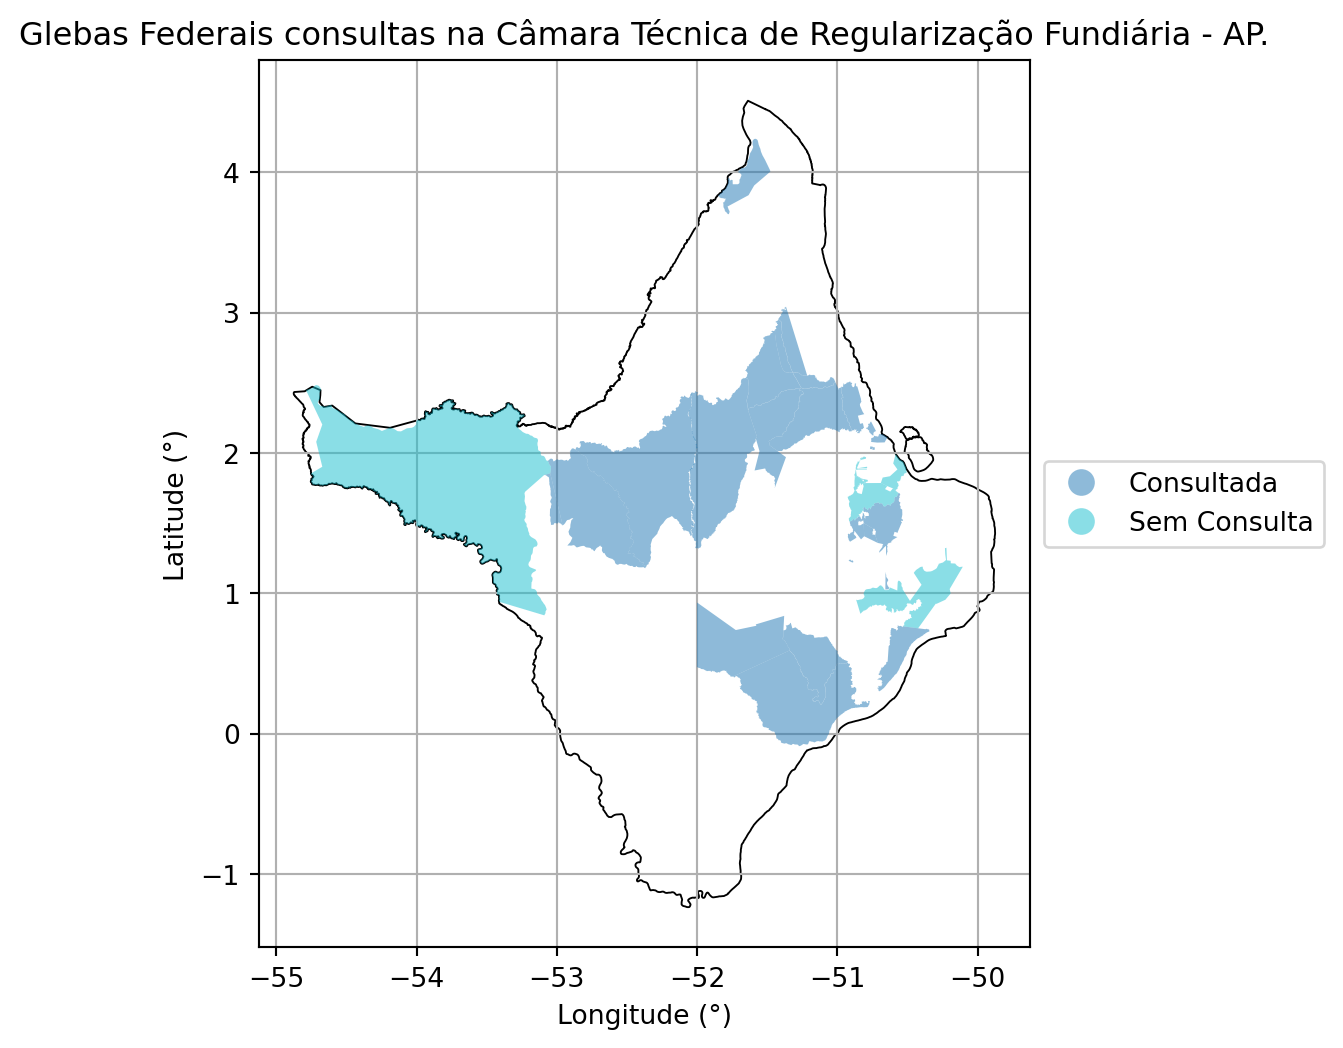
\includegraphics{./7-ctrf_files/figure-pdf/cell-5-output-8.pdf}

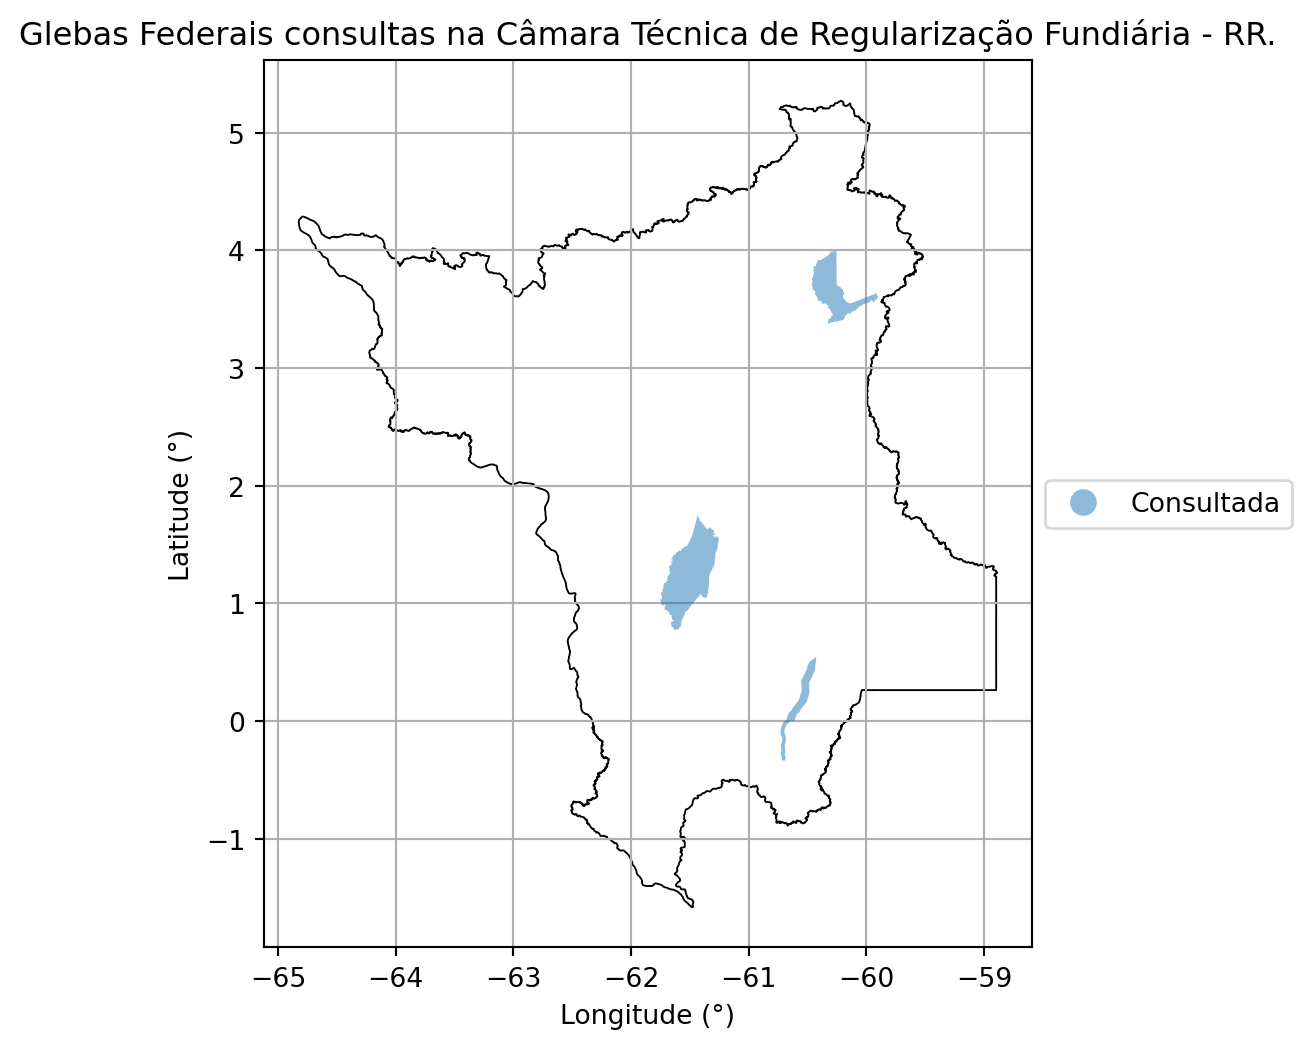
\includegraphics{./7-ctrf_files/figure-pdf/cell-5-output-9.pdf}

\bookmarksetup{startatroot}

\hypertarget{registros-em-cartuxf3rio}{%
\chapter{Registros em Cartório}\label{registros-em-cartuxf3rio}}

A Lei 6.015 que dispõe sobre os registros públicos, e dá outras
providências, estabelece que:

\begin{quote}
Art. 172 - No Registro de Imóveis serão feitos, nos termos desta Lei, o
registro e a averbação dos títulos ou atos constitutivos, declaratórios,
translativos e extintos de direitos reais sobre imóveis reconhecidos em
lei, '' inter vivos'' ou '' mortis causa'' quer para sua constituição,
transferência e extinção, quer para sua validade em relação a terceiros,
quer para a sua disponibilidade.

Art. 176 - O Livro nº 2 - Registro Geral - será destinado, à matrícula
dos imóveis e ao registro ou averbação dos atos relacionados no art. 167
e não atribuídos ao Livro nº 3.

§ 1º A escrituração do Livro nº 2 obedecerá às seguintes normas:

I - cada imóvel terá matrícula própria, que será aberta por ocasião do
primeiro ato de registro ou de averbação caso a transcrição possua todos
os requisitos elencados para a abertura de matrícula;

II - são requisitos da matrícula:

\begin{enumerate}
\def\labelenumi{\arabic{enumi})}
\item
  o número de ordem, que seguirá ao infinito;
\item
  a data;
\item
  a identificação do imóvel, que será feita com indicação: a - se rural,
  do código do imóvel, dos dados constantes do CCIR, da denominação e de
  suas características, confrontações, localização e área; b - se
  urbano, de suas características e confrontações, localização, área,
  logradouro, número e de sua designação cadastral, se houver.
\item
  o nome, domicílio e nacionalidade do proprietário, bem como:

  \begin{enumerate}
  \def\labelenumii{\alph{enumii})}
  \tightlist
  \item
    tratando-se de pessoa física, o estado civil, a profissão, o número
    de inscrição no Cadastro de Pessoas Físicas do Ministério da Fazenda
    ou do Registro Geral da cédula de identidade, ou à falta deste, sua
    filiação;
  \item
    tratando-se de pessoa jurídica, a sede social e o número de
    inscrição no Cadastro Geral de Contribuintes do Ministério da
    Fazenda;
  \end{enumerate}
\item
  o número do registro anterior;
\item
  tratando-se de imóvel em regime de multipropriedade, a indicação da
  existência de matrículas, nos termos do § 10 deste artigo;
\end{enumerate}

III - são requisitos do registro no Livro nº 2:

\begin{enumerate}
\def\labelenumi{\arabic{enumi})}
\item
  a data;
\item
  o nome, domicílio e nacionalidade do transmitente, ou do devedor, e do
  adquirente, ou credor, bem como:

  \begin{enumerate}
  \def\labelenumii{\alph{enumii})}
  \tightlist
  \item
    tratando-se de pessoa física, o estado civil, a profissão e o número
    de inscrição no Cadastro de Pessoas Físicas do Ministério da Fazenda
    ou do Registro Geral da cédula de identidade, ou, à falta deste, sua
    filiação;
  \item
    tratando-se de pessoa jurídica, a sede social e o número de
    inscrição no Cadastro Geral de Contribuintes do Ministério da
    Fazenda;
  \end{enumerate}
\item
  o título da transmissão ou do ônus;
\item
  a forma do título, sua procedência e caracterização;
\item
  o valor do contrato, da coisa ou da dívida, prazo desta, condições e
  mais especificações, inclusive os juros, se houver.
\end{enumerate}
\end{quote}

\begin{center}\rule{0.5\linewidth}{0.5pt}\end{center}

\textbf{Definição de Código Nacional de Serventias (CNS).}

\emph{CNS}: é o Código do Cartório de Registro de Imóveis em que o
imóvel vizinho tem registro, este CNS -- Código Nacional de Serventias.

\begin{center}\rule{0.5\linewidth}{0.5pt}\end{center}

\hypertarget{chave-de-identificauxe7uxe3o-registral-dos-imuxf3veis.}{%
\section{Chave de identificação registral dos
imóveis.}\label{chave-de-identificauxe7uxe3o-registral-dos-imuxf3veis.}}

Conforme descrito acima, a identificação registral de um imóvel é
composta por uma chave dupla sendo composta pelo número da matrícula
(que vai de 1 ao infinito) e o Código Nacional de Serventias - CNS, que
identifica o cartório no qual a matrícula foi registrada. Assim, na
tabela de informações sobre as gelbas, duas colunas são necessárias para
identificação registral da gleba.

\emph{\textbf{Matrícula:}} receberá o número da matrícula, R ou AV,
livro e página;

\emph{\textbf{CNS:}} receberá o número correspondente ao Código Nacional
de Serventias do cartório de registro da matrícula.

\hypertarget{anuxe1lise-das-informauxe7uxf5es}{%
\section{Análise das
informações}\label{anuxe1lise-das-informauxe7uxf5es}}

\hypertarget{nuxfamero-de-glebas-com-informauxe7uxf5es-de-matruxedcula-e-cns-do-catuxf3rio-cadastradas.}{%
\subsection{Número de glebas com informações de matrícula e CNS do
Catório
cadastradas.}\label{nuxfamero-de-glebas-com-informauxe7uxf5es-de-matruxedcula-e-cns-do-catuxf3rio-cadastradas.}}

\n  

\n    

\n      

Total de Áreas

\n      

Matrículas Cadastradas

\n      

Matrículas com CNS

\n      

Matrículas Sem Cadastro

\n    

\n  

\n  

\n    

\n      

81

\n      

31

\n      

21

\n      

50

\n    

\n    

\n      

257

\n      

164

\n      

137

\n      

93

\n    

\n    

\n      

31

\n      

15

\n      

11

\n      

16

\n    

\n    

\n      

113

\n      

94

\n      

93

\n      

19

\n    

\n    

\n      

583

\n      

427

\n      

377

\n      

156

\n    

\n    

\n      

410

\n      

272

\n      

131

\n      

138

\n    

\n    

\n      

79

\n      

58

\n      

16

\n      

21

\n    

\n    

\n      

3

\n      

0

\n      

0

\n      

3

\n    

\n    

\n      

544

\n      

61

\n      

49

\n      

483

\n    

\n  

\n

\bookmarksetup{startatroot}

\hypertarget{glebas-puxfablicas-federais-por-superintenduxeancia-regional-do-incra.}{%
\chapter{Glebas públicas federais por Superintendência Regional do
INCRA.}\label{glebas-puxfablicas-federais-por-superintenduxeancia-regional-do-incra.}}

\hypertarget{localizauxe7uxe3o-das-superintenduxeancias-regionais-do-incra-dentro-da-uxe1rea-de-estudo.}{%
\section{Localização das superintendências Regionais do INCRA dentro da
área de
estudo.}\label{localizauxe7uxe3o-das-superintenduxeancias-regionais-do-incra-dentro-da-uxe1rea-de-estudo.}}

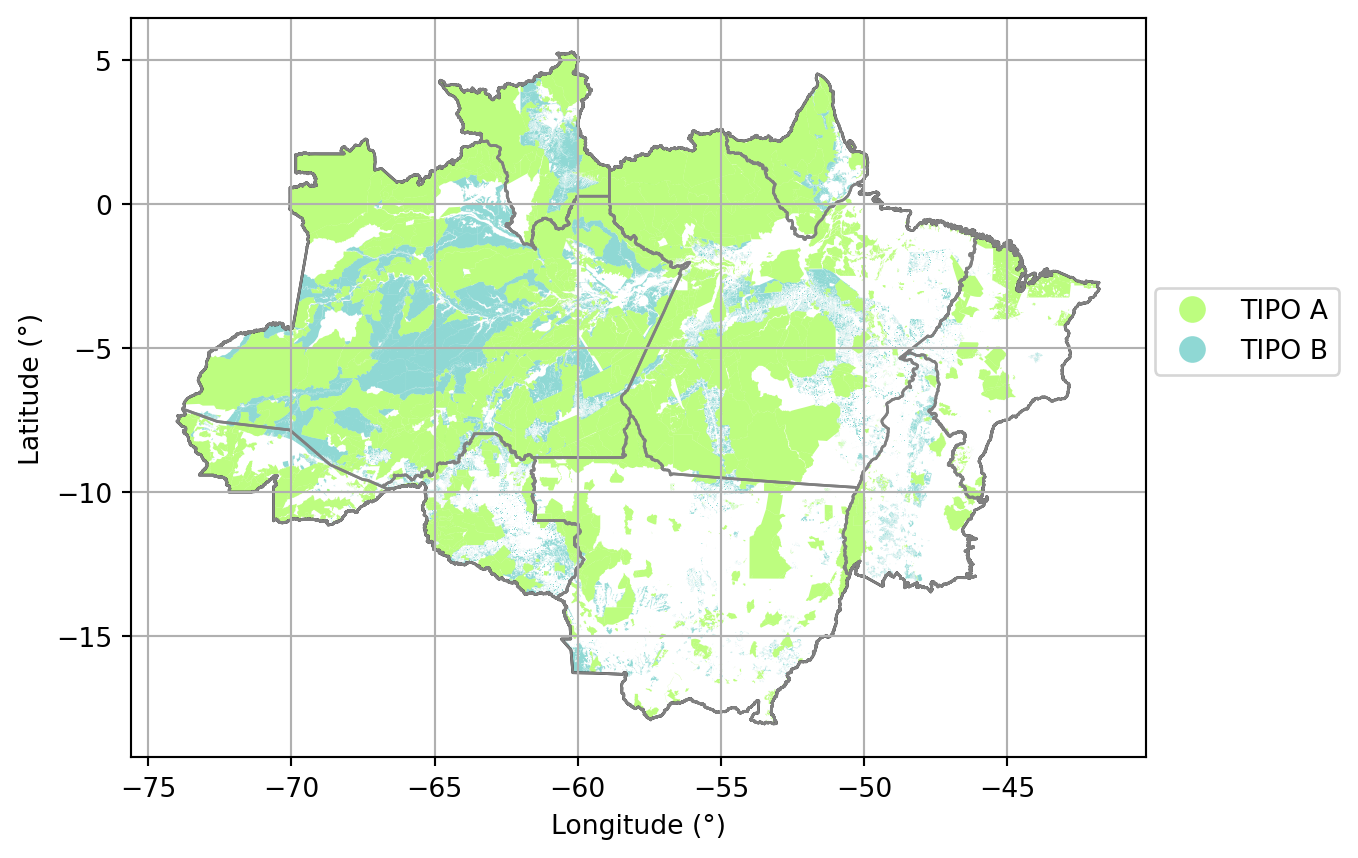
\includegraphics{./9-sr_files/figure-pdf/cell-3-output-1.pdf}

\hypertarget{superintenduxeancias-regionais-do-incra.}{%
\section{Superintendências Regionais do
INCRA.}\label{superintenduxeancias-regionais-do-incra.}}

\begin{longtable}[]{@{}
  >{\centering\arraybackslash}p{(\columnwidth - 12\tabcolsep) * \real{0.1281}}
  >{\centering\arraybackslash}p{(\columnwidth - 12\tabcolsep) * \real{0.3202}}
  >{\centering\arraybackslash}p{(\columnwidth - 12\tabcolsep) * \real{0.0690}}
  >{\centering\arraybackslash}p{(\columnwidth - 12\tabcolsep) * \real{0.0246}}
  >{\raggedright\arraybackslash}p{(\columnwidth - 12\tabcolsep) * \real{0.0591}}
  >{\centering\arraybackslash}p{(\columnwidth - 12\tabcolsep) * \real{0.1921}}
  >{\centering\arraybackslash}p{(\columnwidth - 12\tabcolsep) * \real{0.2069}}@{}}
\toprule()
\begin{minipage}[b]{\linewidth}\centering
Superintendência
\end{minipage} & \begin{minipage}[b]{\linewidth}\centering
Endereço
\end{minipage} & \begin{minipage}[b]{\linewidth}\centering
Cidade
\end{minipage} & \begin{minipage}[b]{\linewidth}\centering
UF
\end{minipage} & \begin{minipage}[b]{\linewidth}\raggedright
CEP
\end{minipage} & \begin{minipage}[b]{\linewidth}\centering
Telefone
\end{minipage} & \begin{minipage}[b]{\linewidth}\centering
\end{minipage} \\
\midrule()
\endhead
Acre & Rua Santa Inês, nº 135 - Bairro Aviário & Rio Branco & AC &
69.900-878 & (68) 3214-3013/ 3086 & \\
Amapá & Rua Adilson José Pinto Pereira, 1409 - Bairro São Lázaro &
Macapá & AP & 68.908-571 & (96) 99107-6937 e (96) 98101-3828 & \\
Amazonas & Av. André Araújo, 901 - Aleixo & Manaus & AM & 69.060-001 &
(92) 3194-1303 & \\
Maranhão & Rua H, Quadra E, Lote 01, N° 12 - Bairro Turu & São Luís & MA
& 65067-150 & (98) 3878-7450 & \\
Mato Grosso & Rua E, s/n - Centro Político Administrativo & Cuiabá & MT
& 78.050-970 & (65) 3644-1104 & \\
Pará - Nordeste (Belém) & Rodovia Murucutum, s/nº - Bairro: Curió-Utinga
Estrada da Ceasa & Belém & PA & 66.610-903 & (91) 3202-3820 & \\
Pará - Oeste (Santarém) & Av. Presidente Vargas, s/nº - Bairro Fátima &
Santarém & PA & 68.040-060 & (93) 3523-1296 & \\
Pará - Sudeste (Marabá) & Avenida Amazônia, s/nº, Agropólis do Incra -
Bairro Amapá & Marabá & PA & 68.502-090 & (94) 3324-1752 & \\
Rondônia & Av. Lauro Sodré, nº 3050 - Bairro Costa e Silva & Porto Velho
& RO & 76.803-488 & (69) 3229-1545 (69) 3229-1691 / 1876 & \\
Tocantins & 302 Norte, Alameda 01, Lote 01 A, Palmas & Palmas & TO &
77.006-336 & (63) 3219-5200/ 5201/ 5240 & \\
\bottomrule()
\end{longtable}

\hypertarget{mapas-de-ligauxe7uxe3o-entre-as-glebas-e-as-superintenduxeancias-regionais.}{%
\section{Mapas de ligação entre as glebas e as Superintendências
Regionais.}\label{mapas-de-ligauxe7uxe3o-entre-as-glebas-e-as-superintenduxeancias-regionais.}}

Os mapas abaixo mostram as distribuições de distâncias dos centroides
das gelbas federais em relação à superintendência regional do INCRA na
qual está sua sede administrativa.

\hypertarget{superintenduxeancia-regional-do-acre.}{%
\subsection{Superintendência Regional do
Acre.}\label{superintenduxeancia-regional-do-acre.}}

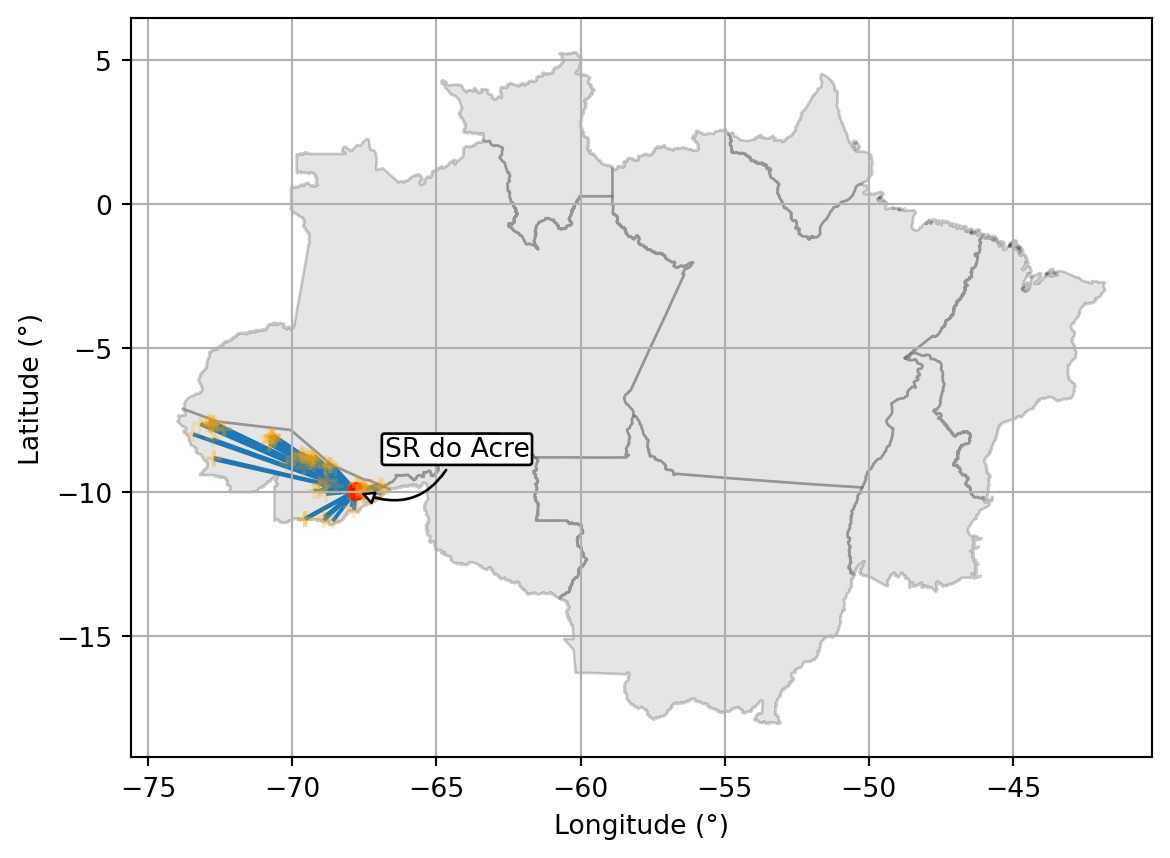
\includegraphics{./9-sr_files/figure-pdf/cell-4-output-2.pdf}

\hypertarget{superintenduxeancia-regional-do-amapuxe1.}{%
\subsection{Superintendência Regional do
Amapá.}\label{superintenduxeancia-regional-do-amapuxe1.}}

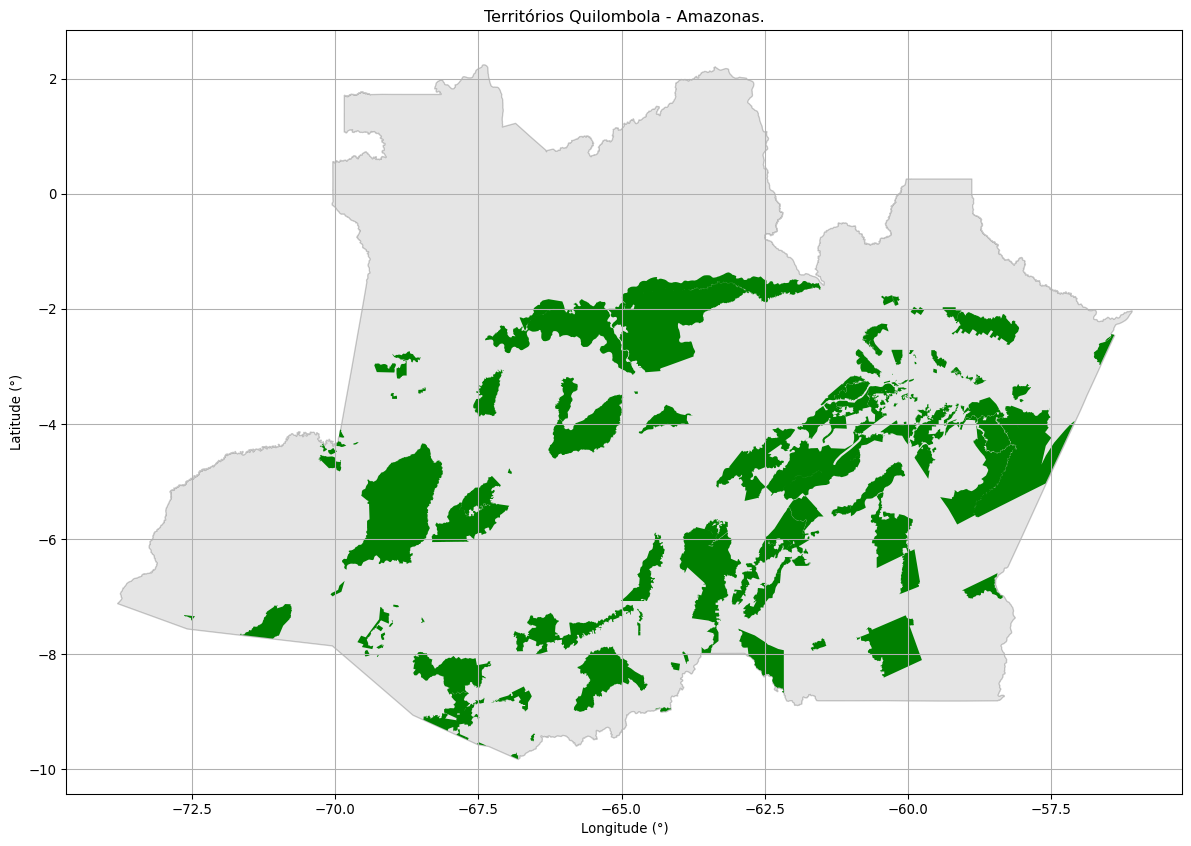
\includegraphics{./9-sr_files/figure-pdf/cell-4-output-4.pdf}

\hypertarget{superintenduxeancia-regional-do-amazonas.}{%
\subsection{Superintendência Regional do
Amazonas.}\label{superintenduxeancia-regional-do-amazonas.}}

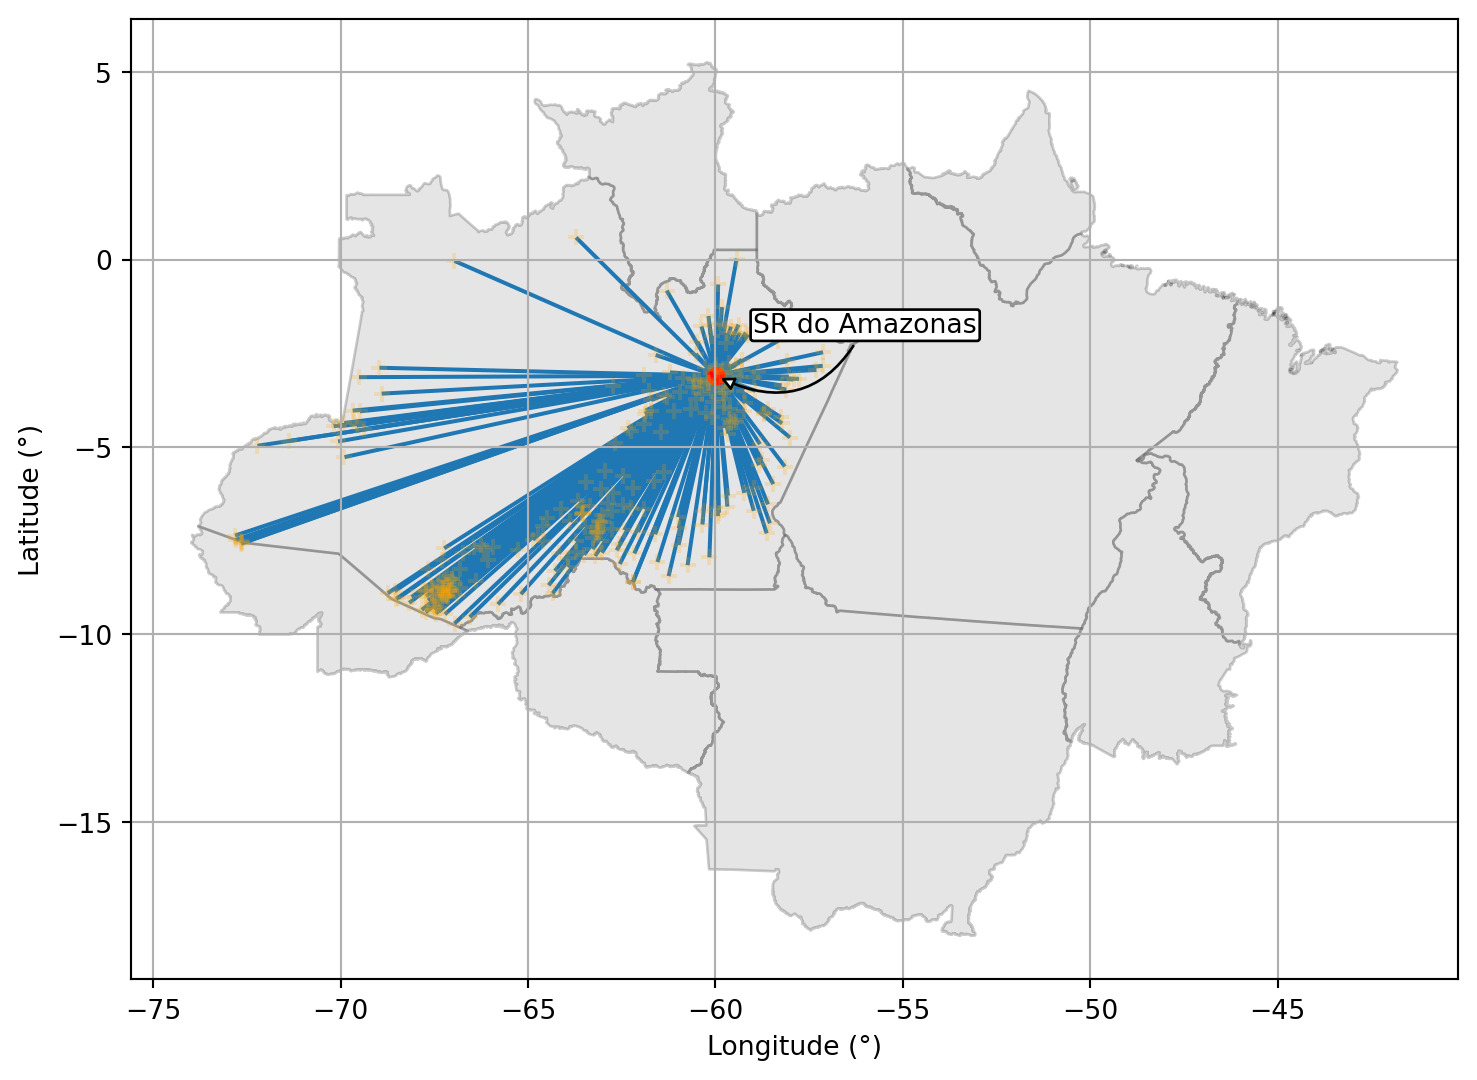
\includegraphics{./9-sr_files/figure-pdf/cell-4-output-6.pdf}

\hypertarget{superintenduxeancia-regional-do-maranhuxe3o.}{%
\subsection{Superintendência Regional do
Maranhão.}\label{superintenduxeancia-regional-do-maranhuxe3o.}}

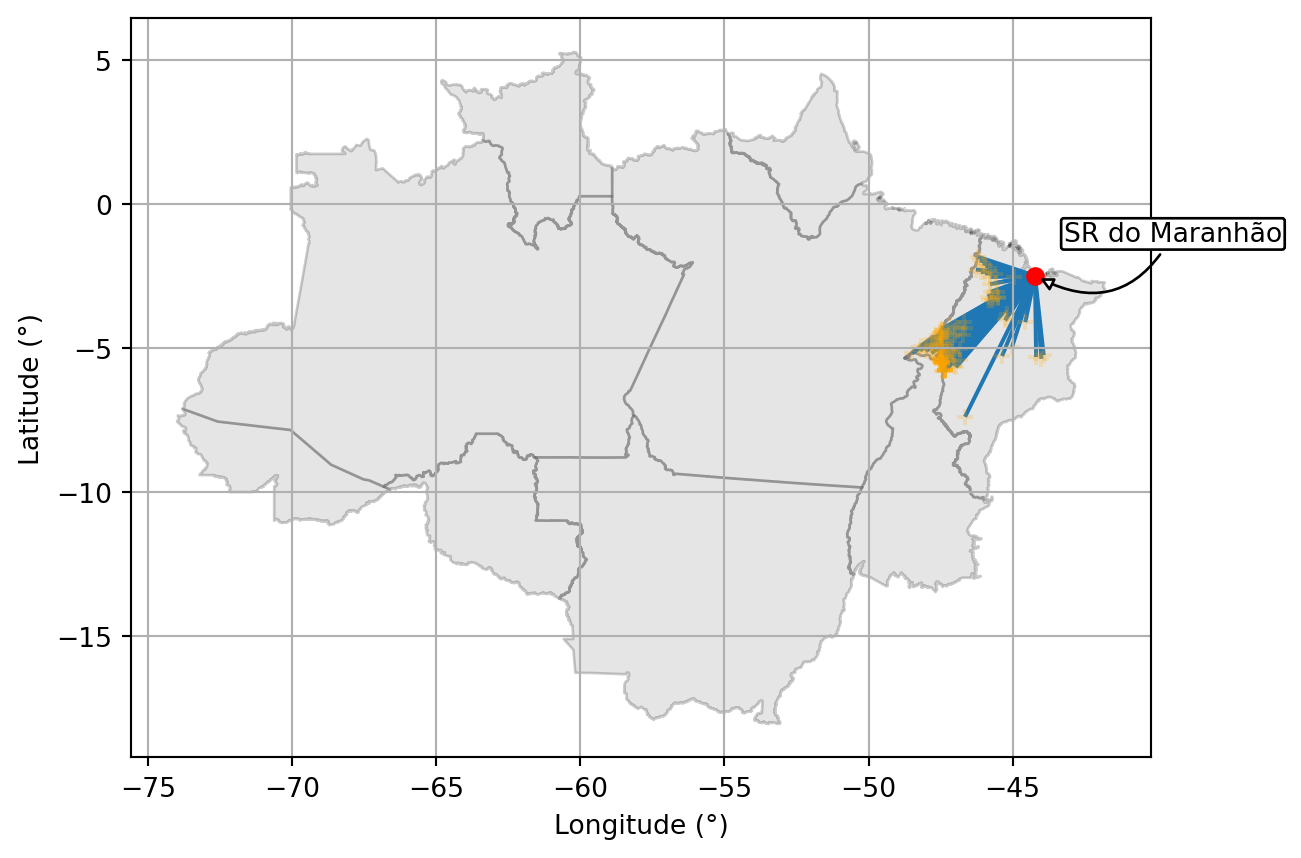
\includegraphics{./9-sr_files/figure-pdf/cell-4-output-8.pdf}

\hypertarget{superintenduxeancia-regional-do-mato-grosso.}{%
\subsection{Superintendência Regional do Mato
Grosso.}\label{superintenduxeancia-regional-do-mato-grosso.}}

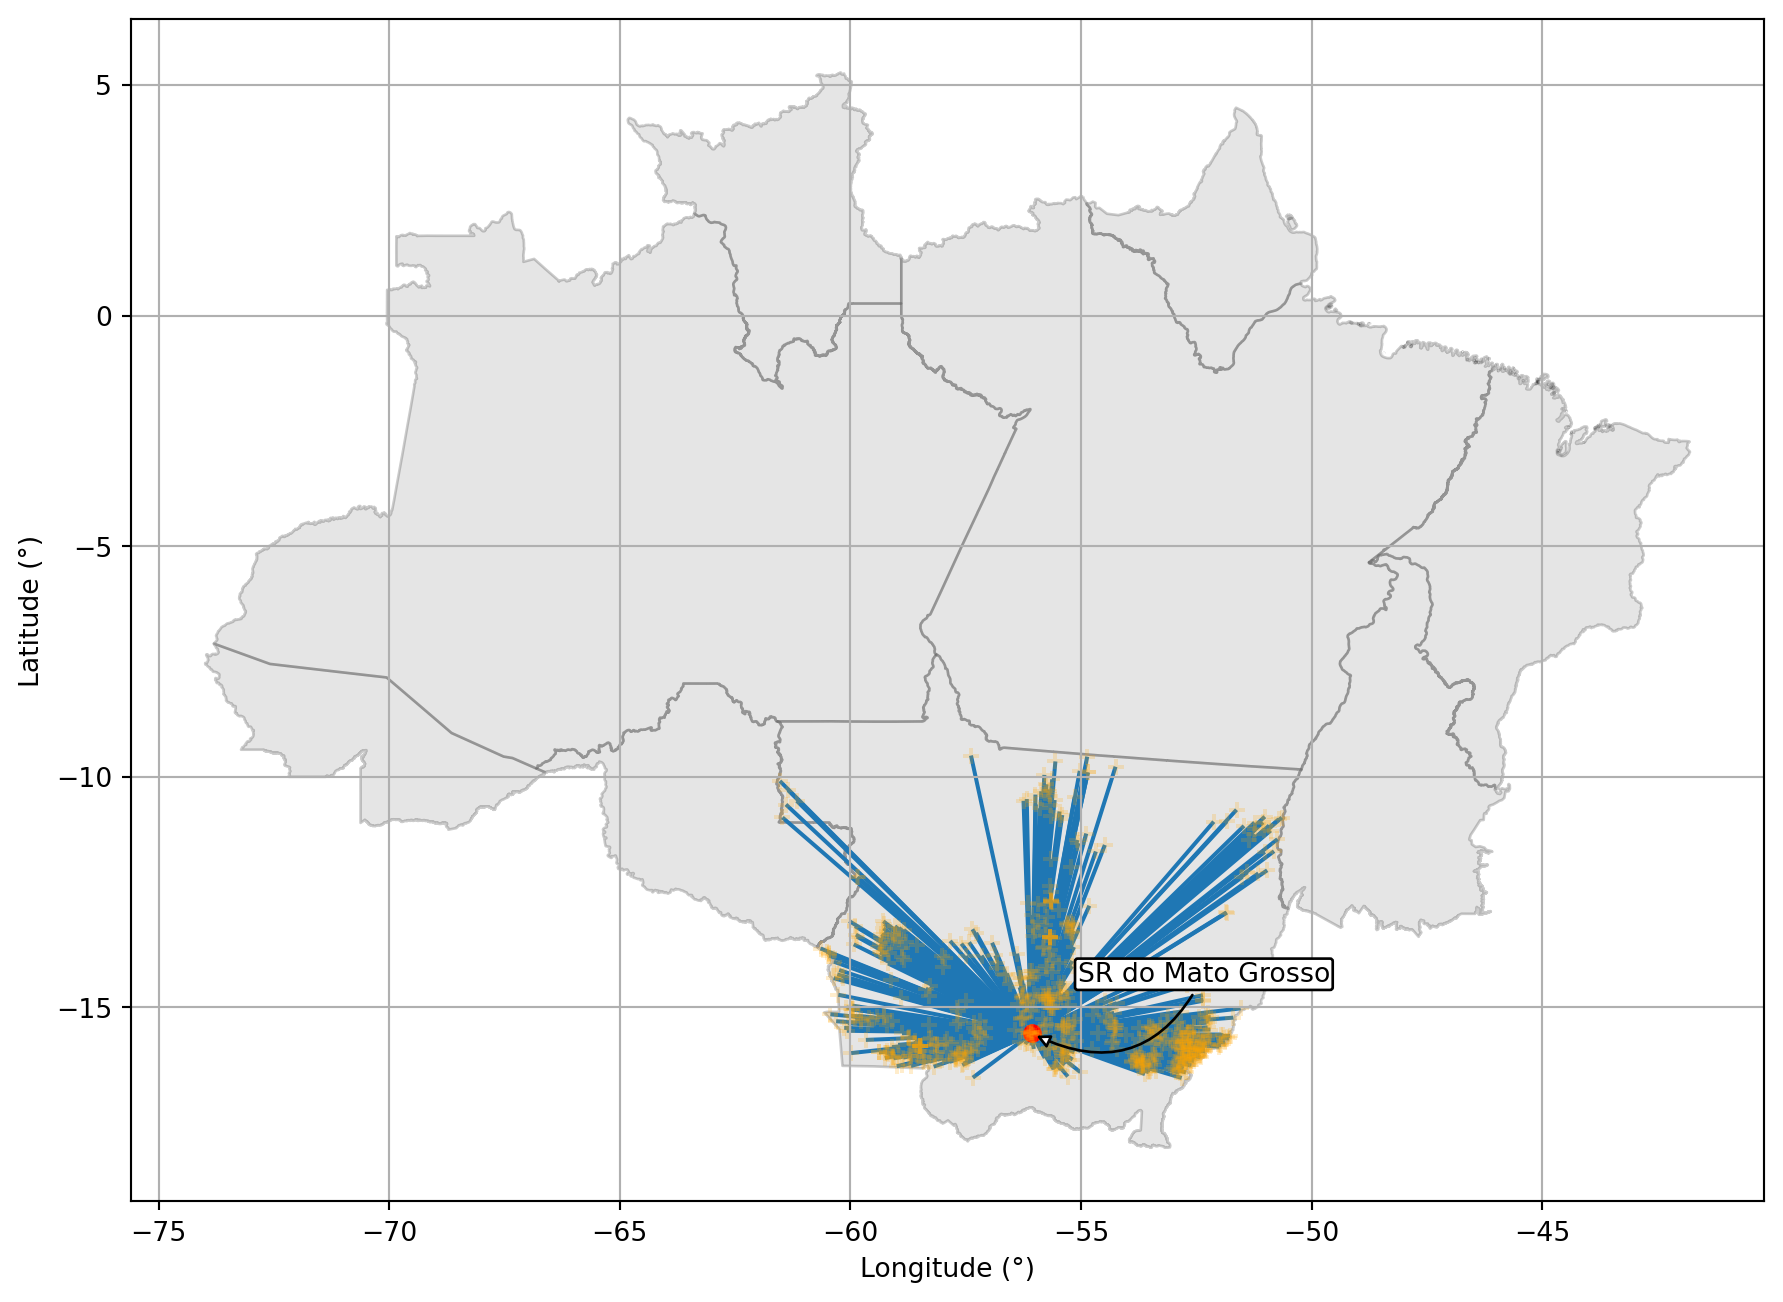
\includegraphics{./9-sr_files/figure-pdf/cell-4-output-10.pdf}

\hypertarget{superintenduxeancia-regional-do-paruxe1---beluxe9m.}{%
\subsection{Superintendência Regional do Pará -
Belém.}\label{superintenduxeancia-regional-do-paruxe1---beluxe9m.}}

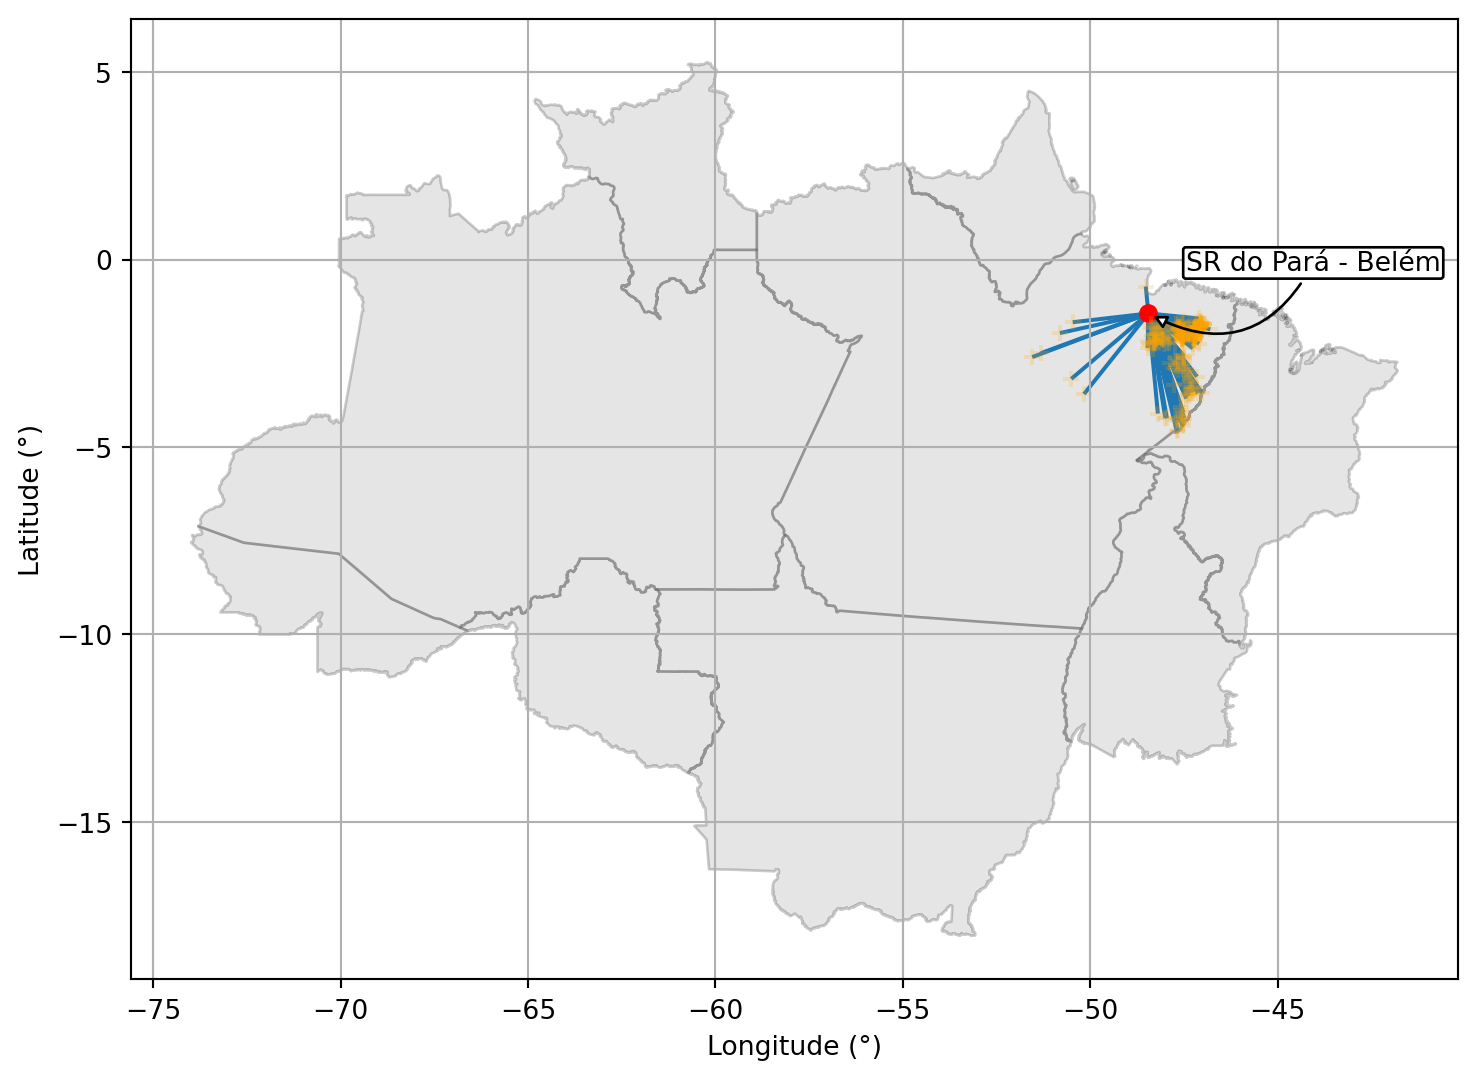
\includegraphics{./9-sr_files/figure-pdf/cell-4-output-12.pdf}

\hypertarget{superintenduxeancia-regional-do-paruxe1---santaruxe9m.}{%
\subsection{Superintendência Regional do Pará -
Santarém.}\label{superintenduxeancia-regional-do-paruxe1---santaruxe9m.}}

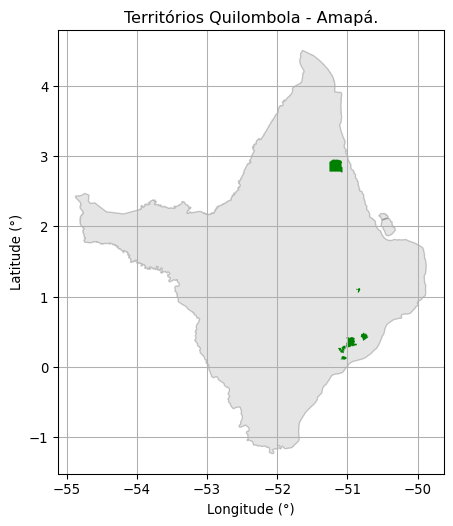
\includegraphics{./9-sr_files/figure-pdf/cell-4-output-14.pdf}

\hypertarget{superintenduxeancia-regional-do-paruxe1---marabuxe1.}{%
\subsection{Superintendência Regional do Pará -
Marabá.}\label{superintenduxeancia-regional-do-paruxe1---marabuxe1.}}

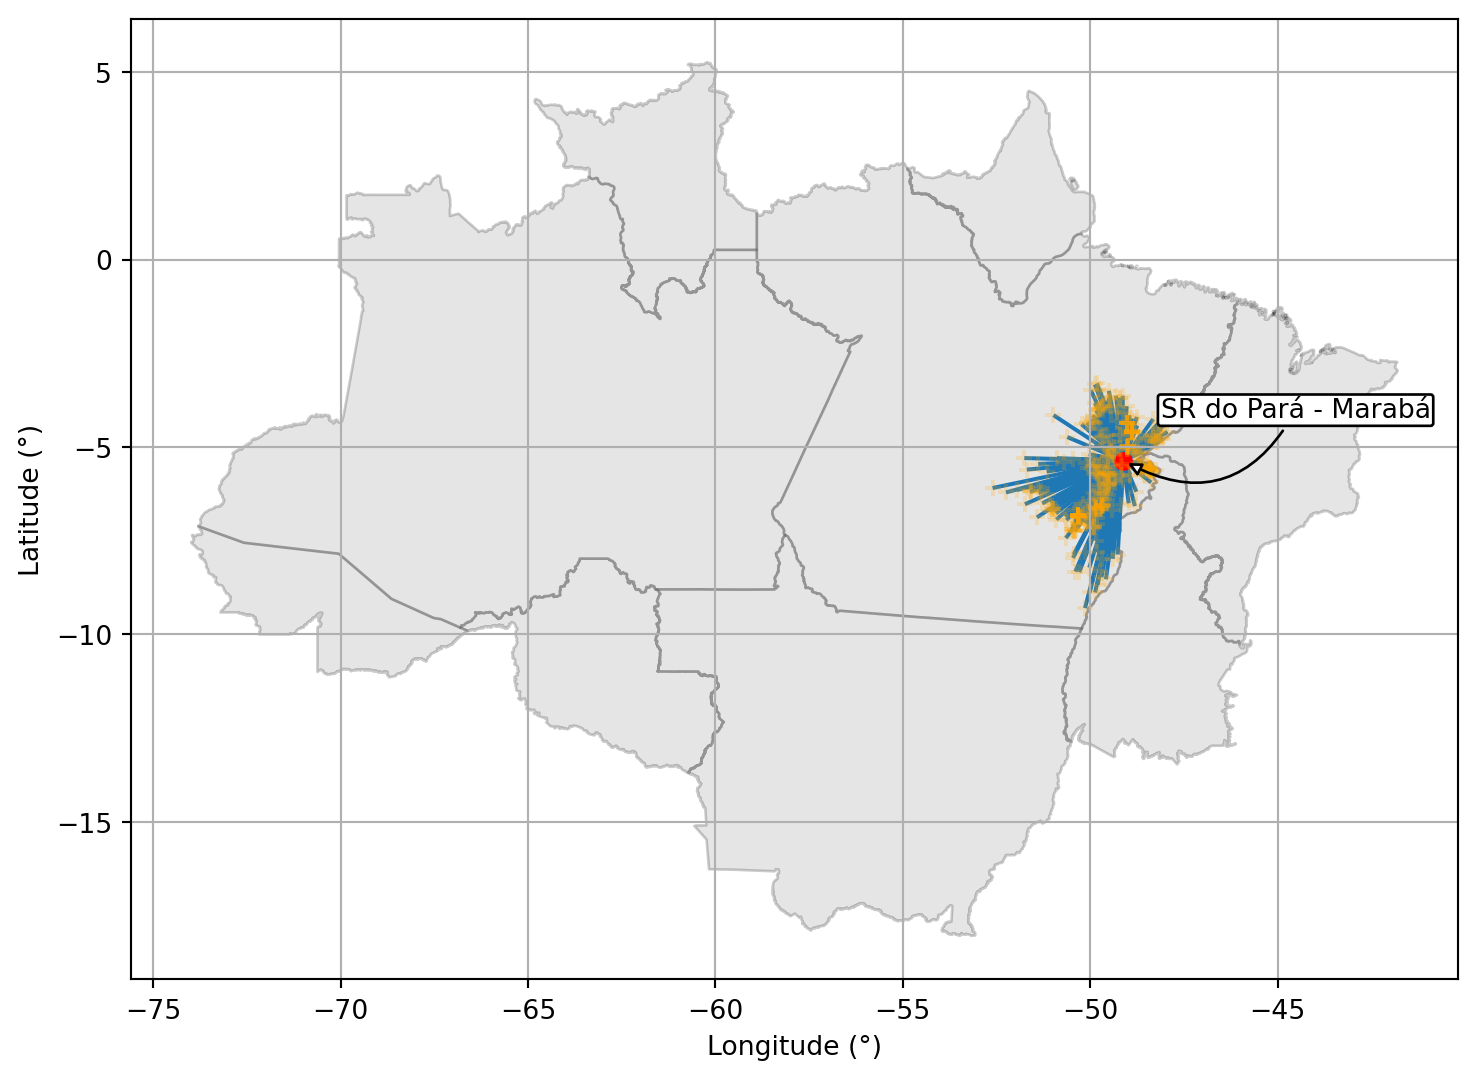
\includegraphics{./9-sr_files/figure-pdf/cell-4-output-16.pdf}

\hypertarget{superintenduxeancia-regional-do-ronduxf4nia.}{%
\subsection{Superintendência Regional do
Rondônia.}\label{superintenduxeancia-regional-do-ronduxf4nia.}}

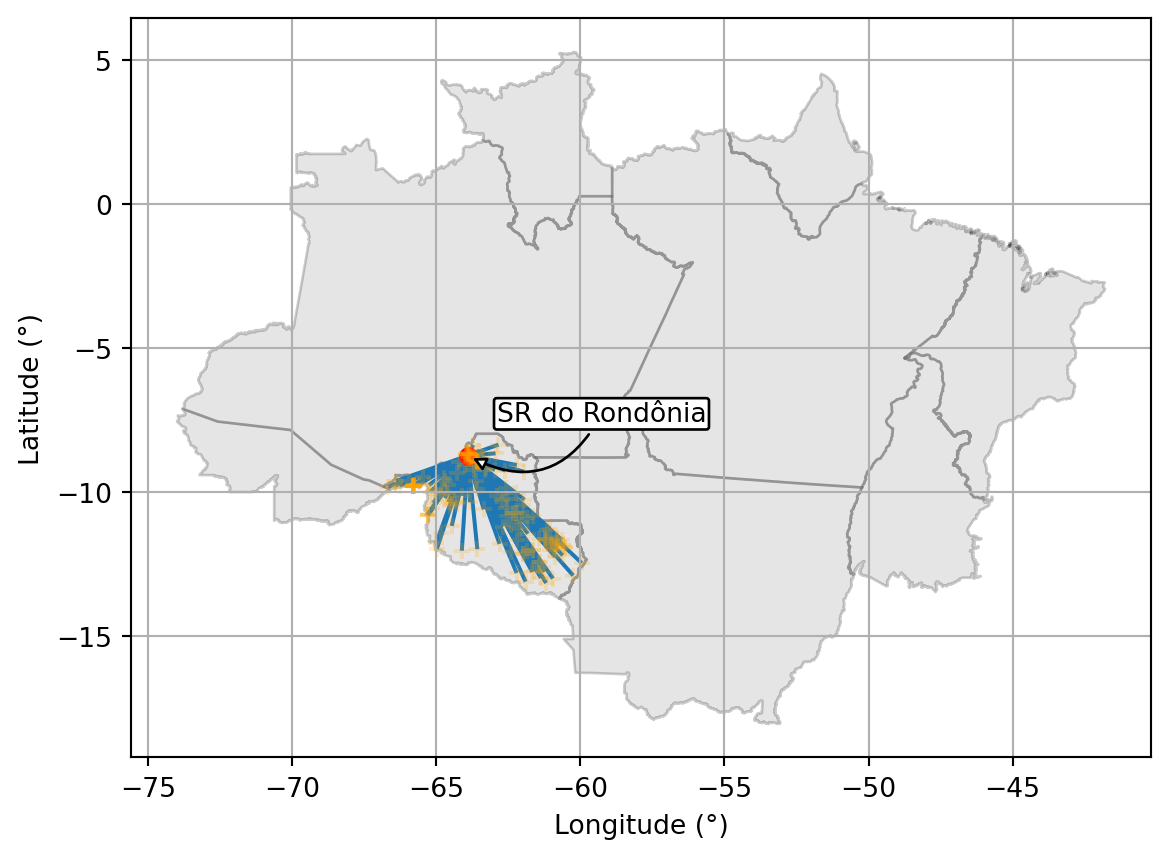
\includegraphics{./9-sr_files/figure-pdf/cell-4-output-18.pdf}

\hypertarget{superintenduxeancia-regional-do-tocantins.}{%
\subsection{Superintendência Regional do
Tocantins.}\label{superintenduxeancia-regional-do-tocantins.}}

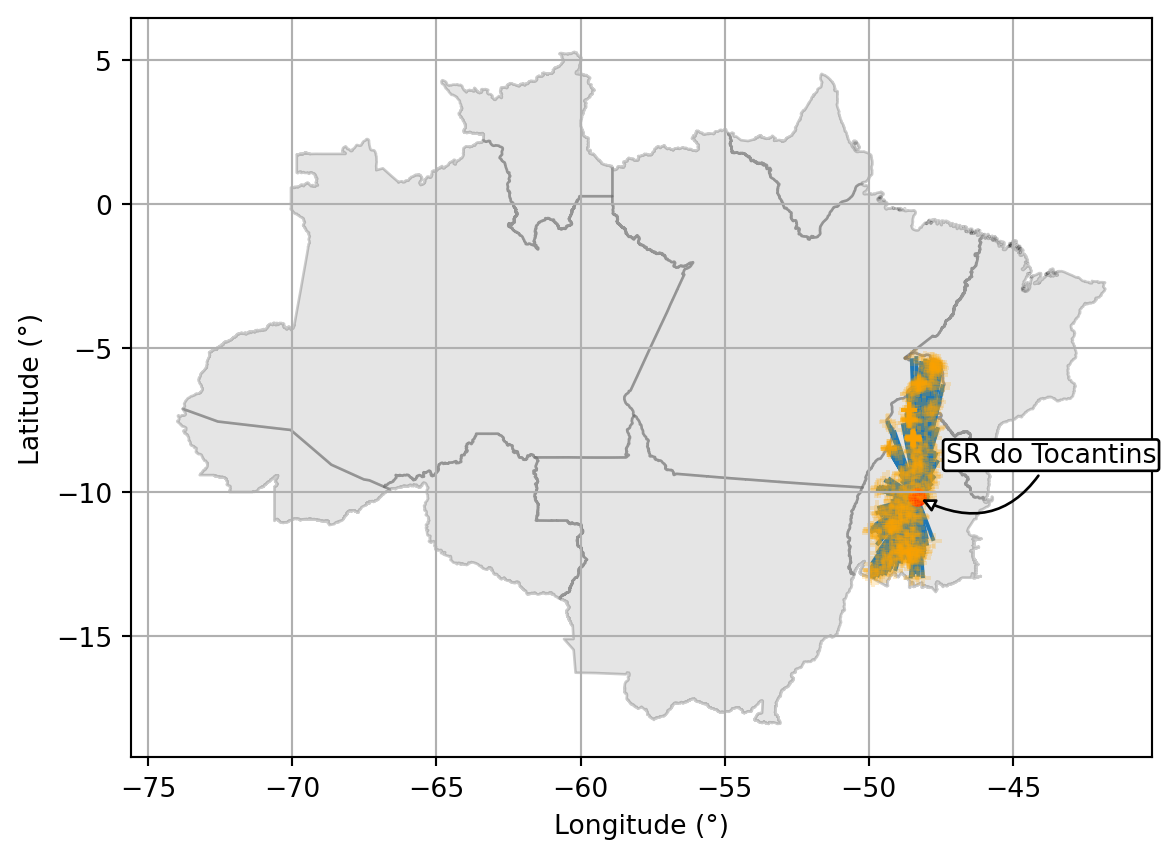
\includegraphics{./9-sr_files/figure-pdf/cell-4-output-20.pdf}

\hypertarget{superintenduxeancia-regional-do-roraima.}{%
\subsection{Superintendência Regional do
Roraima.}\label{superintenduxeancia-regional-do-roraima.}}

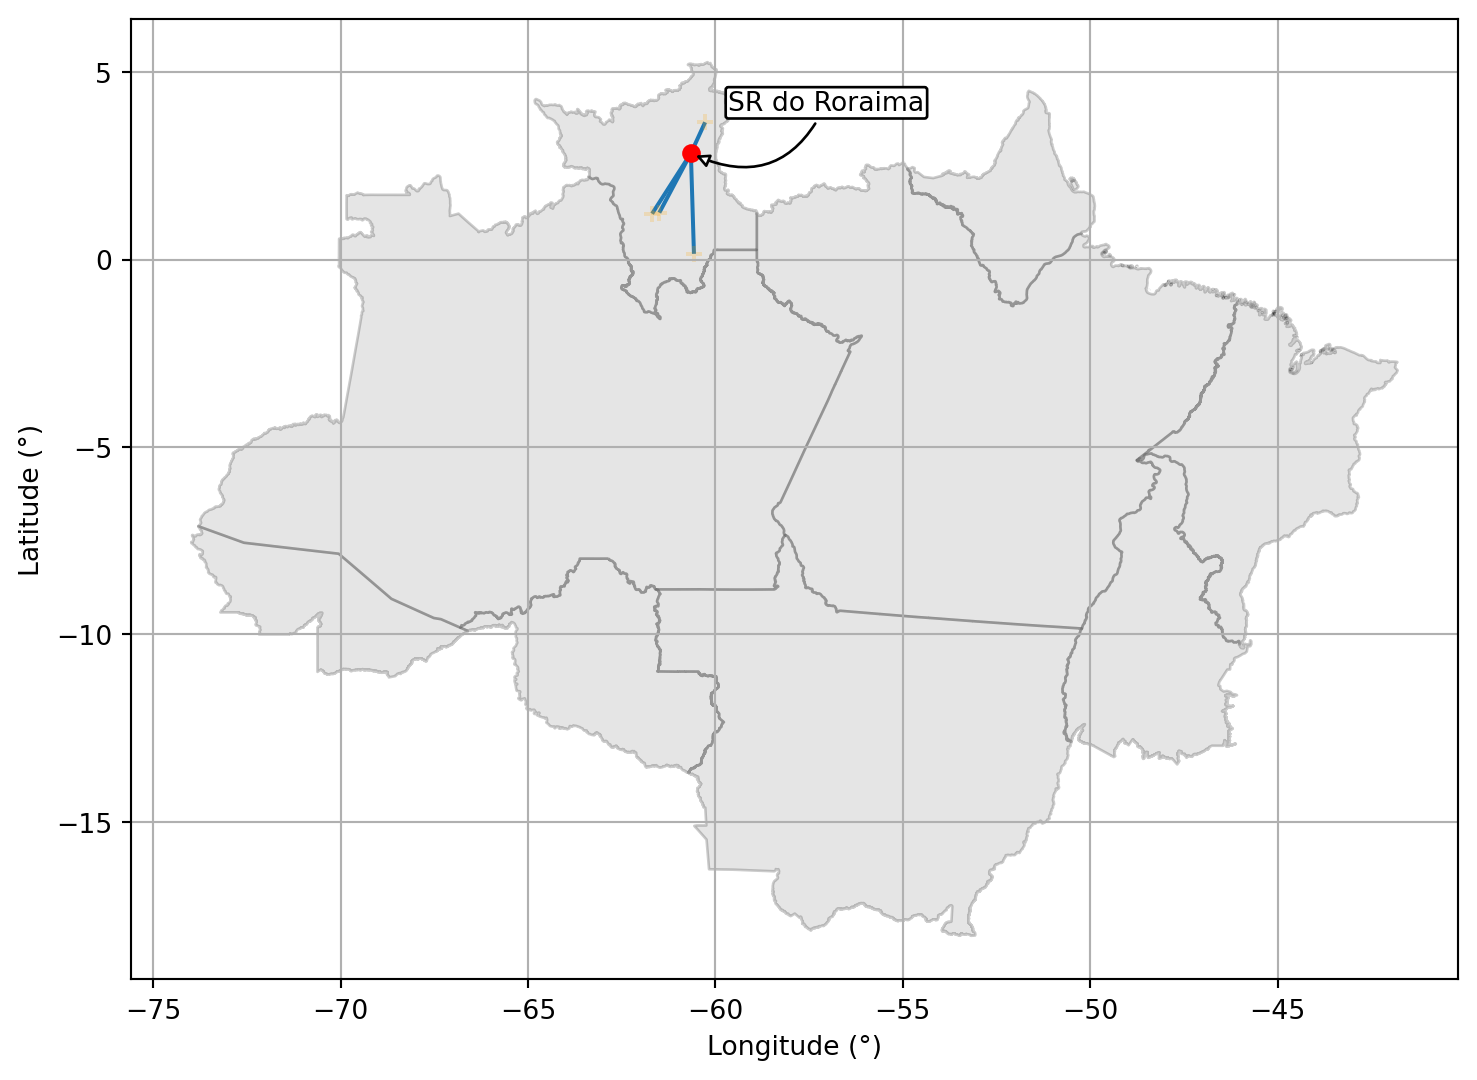
\includegraphics{./9-sr_files/figure-pdf/cell-4-output-22.pdf}

\hypertarget{distuxe2ncias-muxe9dias-e-muxe1ximas-das-glebas-em-relauxe7uxe3o-uxe0-sua-superintenduxeancia-regional-do-incra.}{%
\subsection{Distâncias médias e máximas das glebas em relação à sua
Superintendência Regional do
INCRA.}\label{distuxe2ncias-muxe9dias-e-muxe1ximas-das-glebas-em-relauxe7uxe3o-uxe0-sua-superintenduxeancia-regional-do-incra.}}

\n  

\n    

\n      

Superintendência

\n      

Distância Máxima (km)

\n      

Distância Média (km)

\n    

\n  

\n  

\n    

\n      

Acre

\n      

658

\n      

237

\n    

\n    

\n      

Amapá

\n      

434

\n      

211

\n    

\n    

\n      

Amazonas

\n      

1500

\n      

565

\n    

\n    

\n      

Maranhão

\n      

604

\n      

395

\n    

\n    

\n      

Mato Grosso

\n      

847

\n      

301

\n    

\n    

\n      

Pará - Belém

\n      

368

\n      

159

\n    

\n    

\n      

Pará - Marabá

\n      

449

\n      

155

\n    

\n    

\n      

Pará - Santarém

\n      

731

\n      

247

\n    

\n    

\n      

Rondônia

\n      

609

\n      

263

\n    

\n    

\n      

Roraima

\n      

297

\n      

202

\n    

\n    

\n      

Tocantins

\n      

540

\n      

229

\n    

\n  

\n

\hypertarget{redistribuiuxe7uxe3o-das-glebas-nas-superintenduxeancias-por-menor-distuxe2nica.}{%
\section{Redistribuição das glebas nas Superintendências por menor
distânica.}\label{redistribuiuxe7uxe3o-das-glebas-nas-superintenduxeancias-por-menor-distuxe2nica.}}

Os mapas abaixo foram criados levando-se em conta a distribuição das
glebas fedrais nas superintendências mais próximas numa distância em
linha reta, outros fatores devem ser considerados numa possível
redistribuição das unidades administrativas das glebas tais como: forma
de acesso, quantidades de servidores em cada suerintendência, \ldots{}

Uma camada de acessoas roteáveis pode aumentar a precisão na tomada de
decisões tornando possível a utilização de algorítimos para determinar
trajeto mais curto ou mais eficiente, impactando também \textbf{na
diminuição da pegada de carbono} dos trabalhos.

A redistribuição das glebas em locais administrativos mais próximos
pode, não só, beneficiar o INCRA na economia de recursos e diminuição
nos prazos de atendimento quanto aos beneficiários que terão o local
para solicitações e atendimento mais próximo.

\hypertarget{superintenduxeancia-regional-do-acre.-1}{%
\subsection{Superintendência Regional do
Acre.}\label{superintenduxeancia-regional-do-acre.-1}}

\includegraphics{./9-sr_files/figure-pdf/cell-6-output-2.pdf}

\hypertarget{superintenduxeancia-regional-do-amapuxe1.-1}{%
\subsection{Superintendência Regional do
Amapá.}\label{superintenduxeancia-regional-do-amapuxe1.-1}}

\includegraphics{./9-sr_files/figure-pdf/cell-6-output-4.pdf}

\hypertarget{superintenduxeancia-regional-do-amazonas.-1}{%
\subsection{Superintendência Regional do
Amazonas.}\label{superintenduxeancia-regional-do-amazonas.-1}}

\includegraphics{./9-sr_files/figure-pdf/cell-6-output-6.pdf}

\hypertarget{superintenduxeancia-regional-do-maranhuxe3o.-1}{%
\subsection{Superintendência Regional do
Maranhão.}\label{superintenduxeancia-regional-do-maranhuxe3o.-1}}

\includegraphics{./9-sr_files/figure-pdf/cell-6-output-8.pdf}

\hypertarget{superintenduxeancia-regional-do-mato-grosso.-1}{%
\subsection{Superintendência Regional do Mato
Grosso.}\label{superintenduxeancia-regional-do-mato-grosso.-1}}

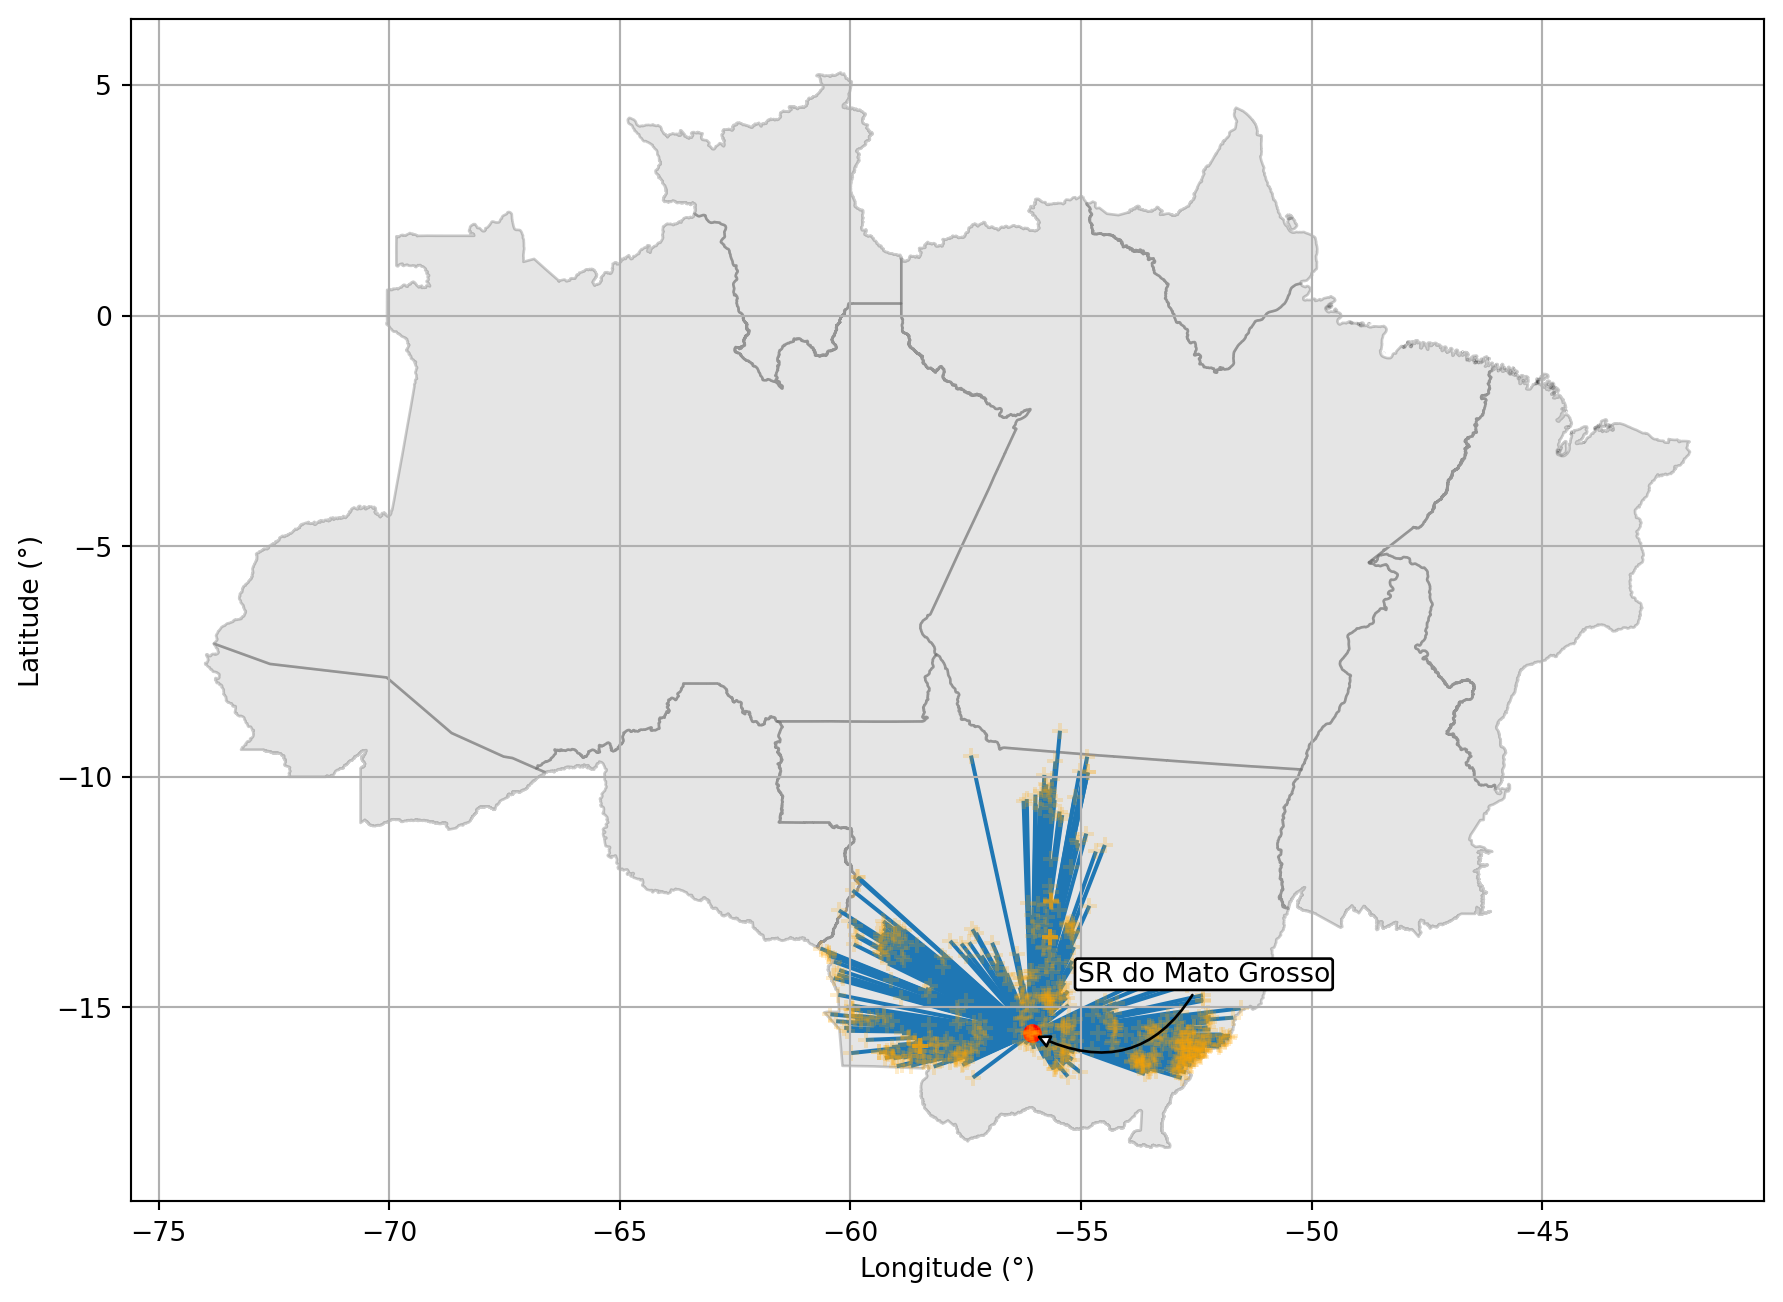
\includegraphics{./9-sr_files/figure-pdf/cell-6-output-10.pdf}

\hypertarget{superintenduxeancia-regional-do-paruxe1---beluxe9m.-1}{%
\subsection{Superintendência Regional do Pará -
Belém.}\label{superintenduxeancia-regional-do-paruxe1---beluxe9m.-1}}

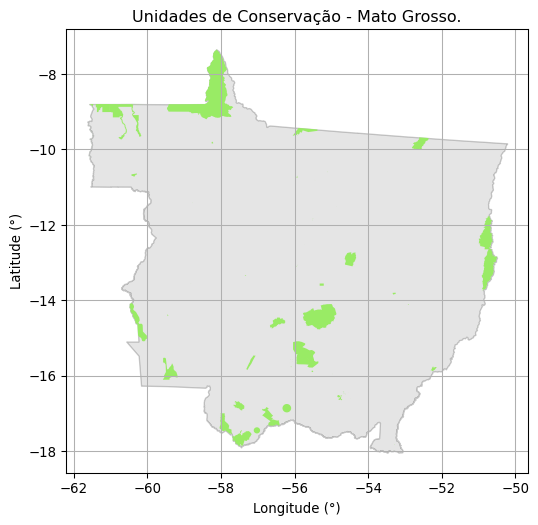
\includegraphics{./9-sr_files/figure-pdf/cell-6-output-12.pdf}

\hypertarget{superintenduxeancia-regional-do-paruxe1---santaruxe9m.-1}{%
\subsection{Superintendência Regional do Pará -
Santarém.}\label{superintenduxeancia-regional-do-paruxe1---santaruxe9m.-1}}

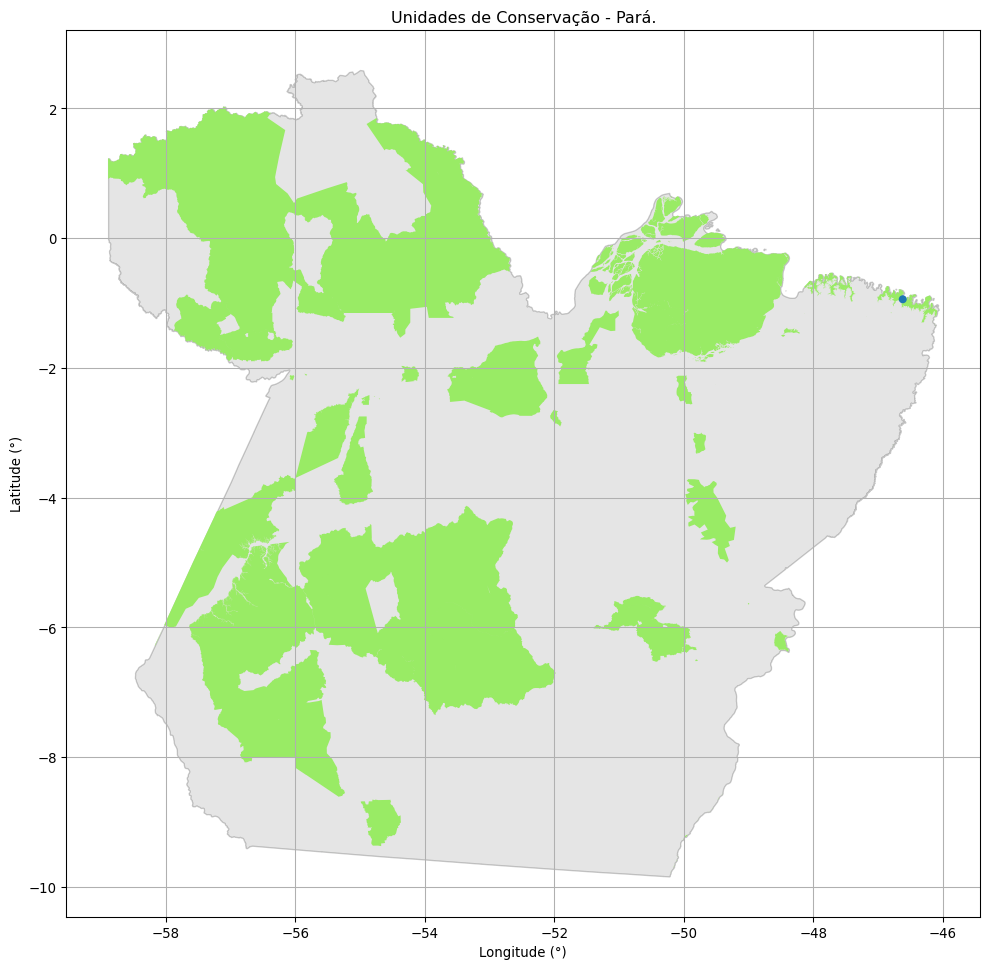
\includegraphics{./9-sr_files/figure-pdf/cell-6-output-14.pdf}

\hypertarget{superintenduxeancia-regional-do-paruxe1---marabuxe1.-1}{%
\subsection{Superintendência Regional do Pará -
Marabá.}\label{superintenduxeancia-regional-do-paruxe1---marabuxe1.-1}}

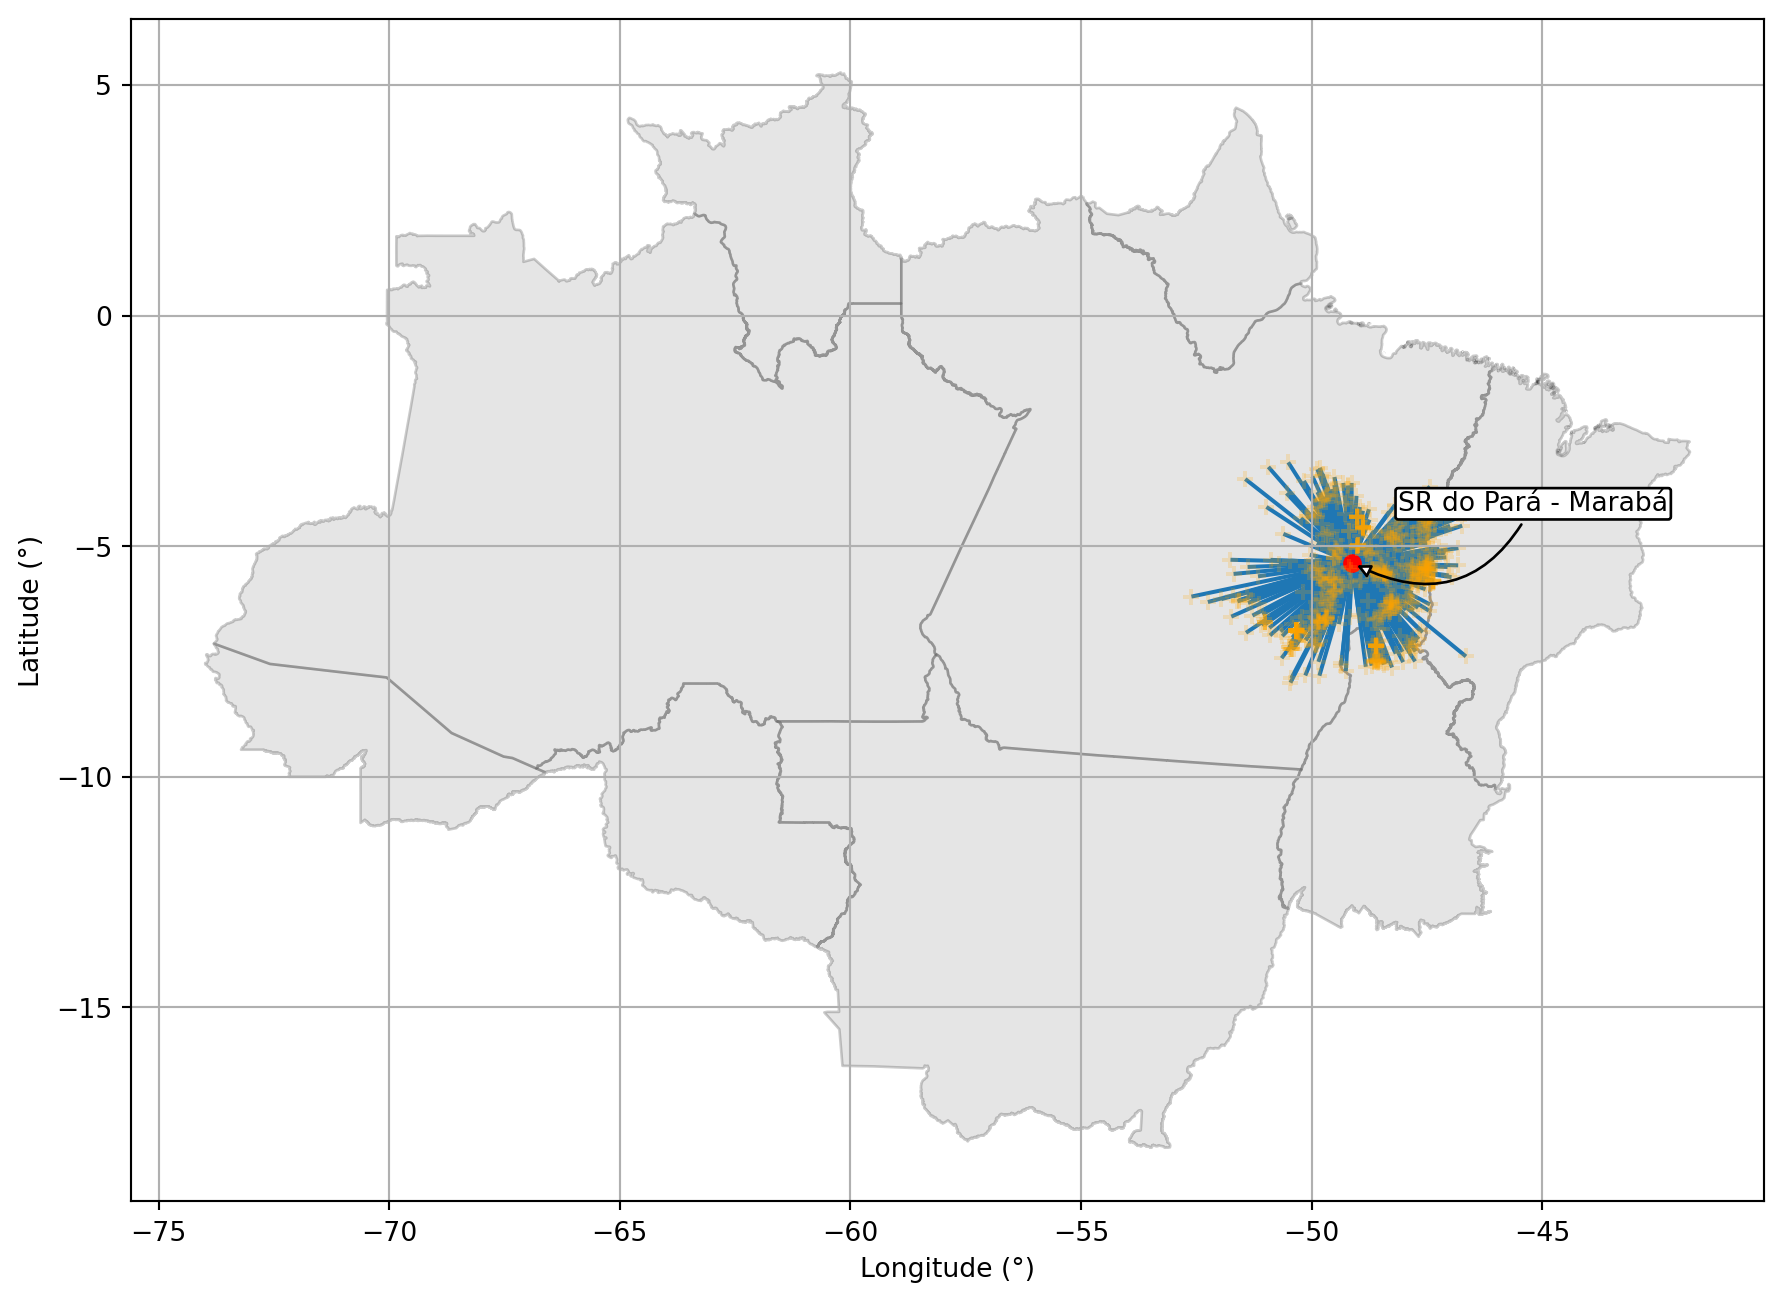
\includegraphics{./9-sr_files/figure-pdf/cell-6-output-16.pdf}

\hypertarget{superintenduxeancia-regional-do-ronduxf4nia.-1}{%
\subsection{Superintendência Regional do
Rondônia.}\label{superintenduxeancia-regional-do-ronduxf4nia.-1}}

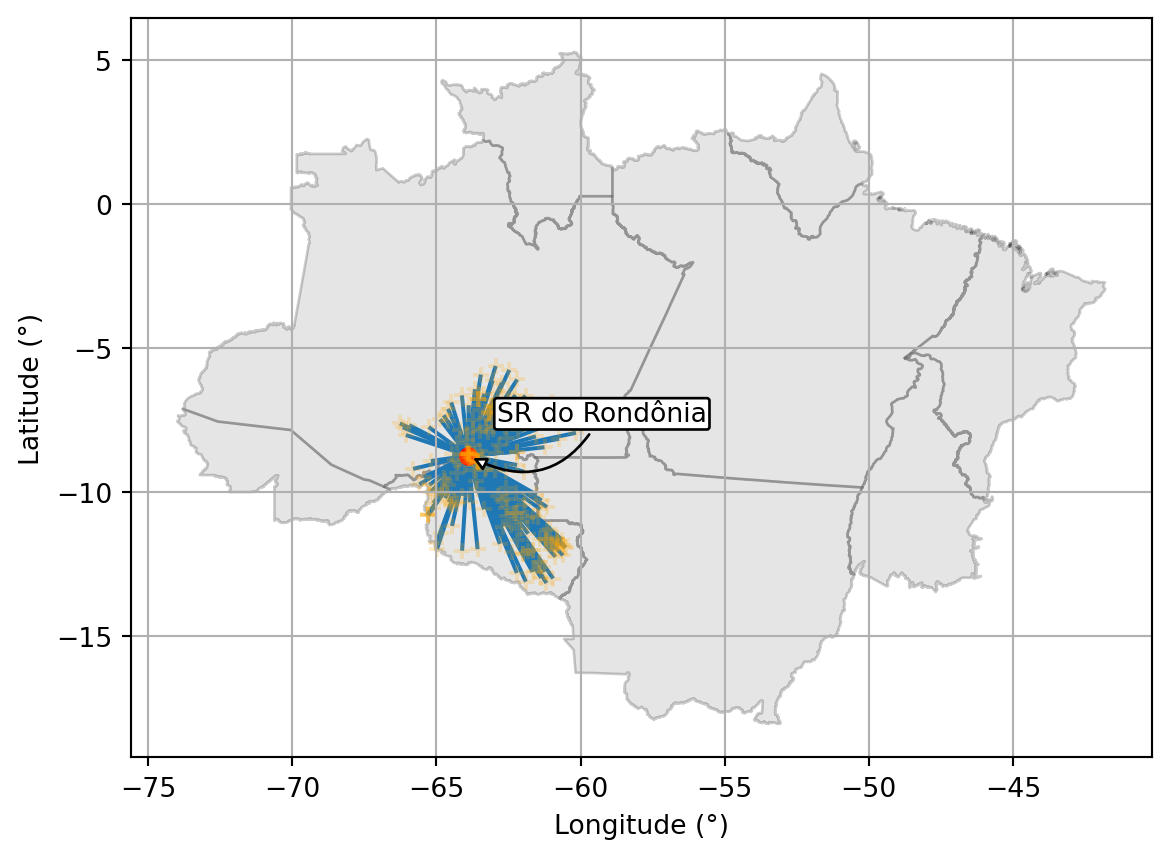
\includegraphics{./9-sr_files/figure-pdf/cell-6-output-18.pdf}

\hypertarget{superintenduxeancia-regional-do-tocantins.-1}{%
\subsection{Superintendência Regional do
Tocantins.}\label{superintenduxeancia-regional-do-tocantins.-1}}

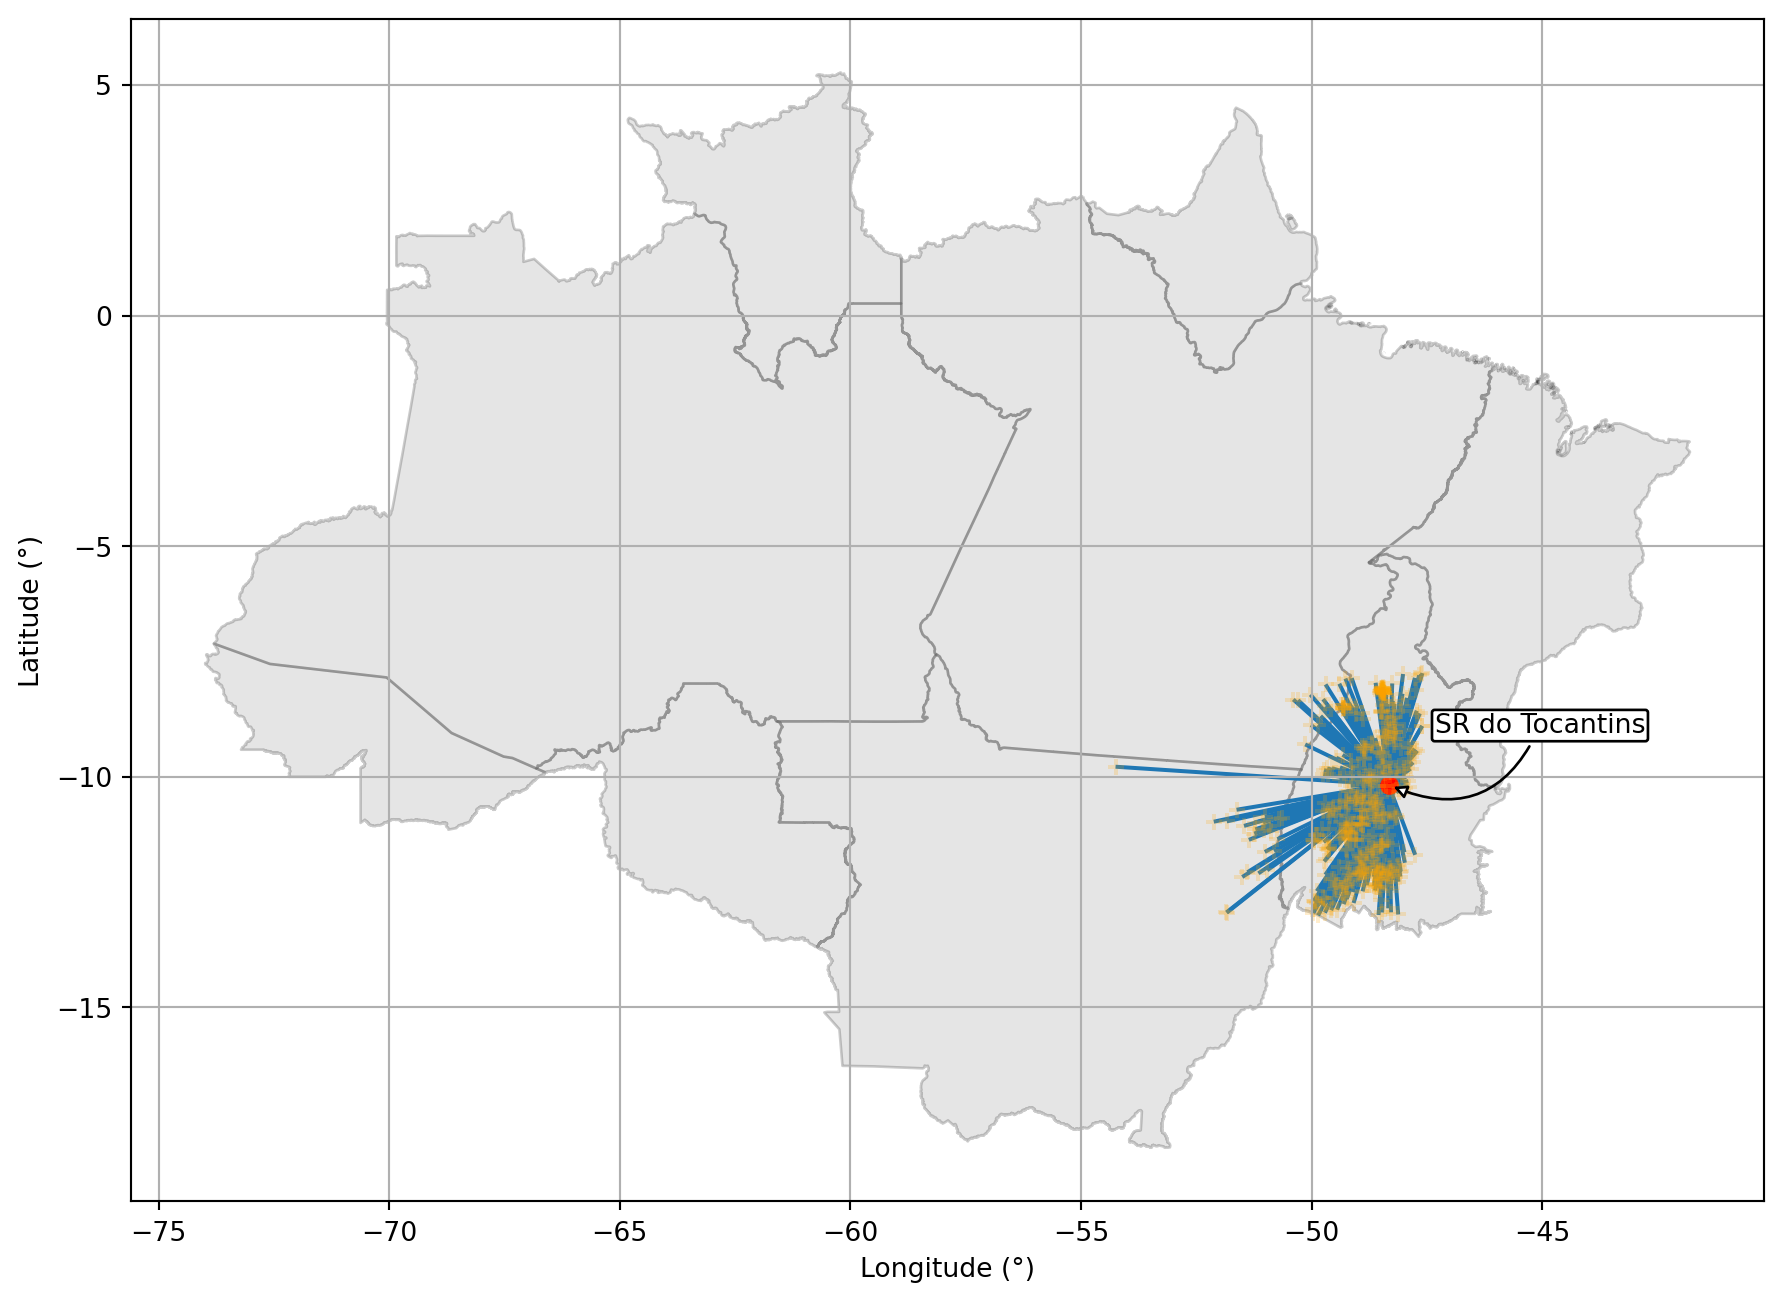
\includegraphics{./9-sr_files/figure-pdf/cell-6-output-20.pdf}

\hypertarget{superintenduxeancia-regional-do-roraima.-1}{%
\subsection{Superintendência Regional do
Roraima.}\label{superintenduxeancia-regional-do-roraima.-1}}

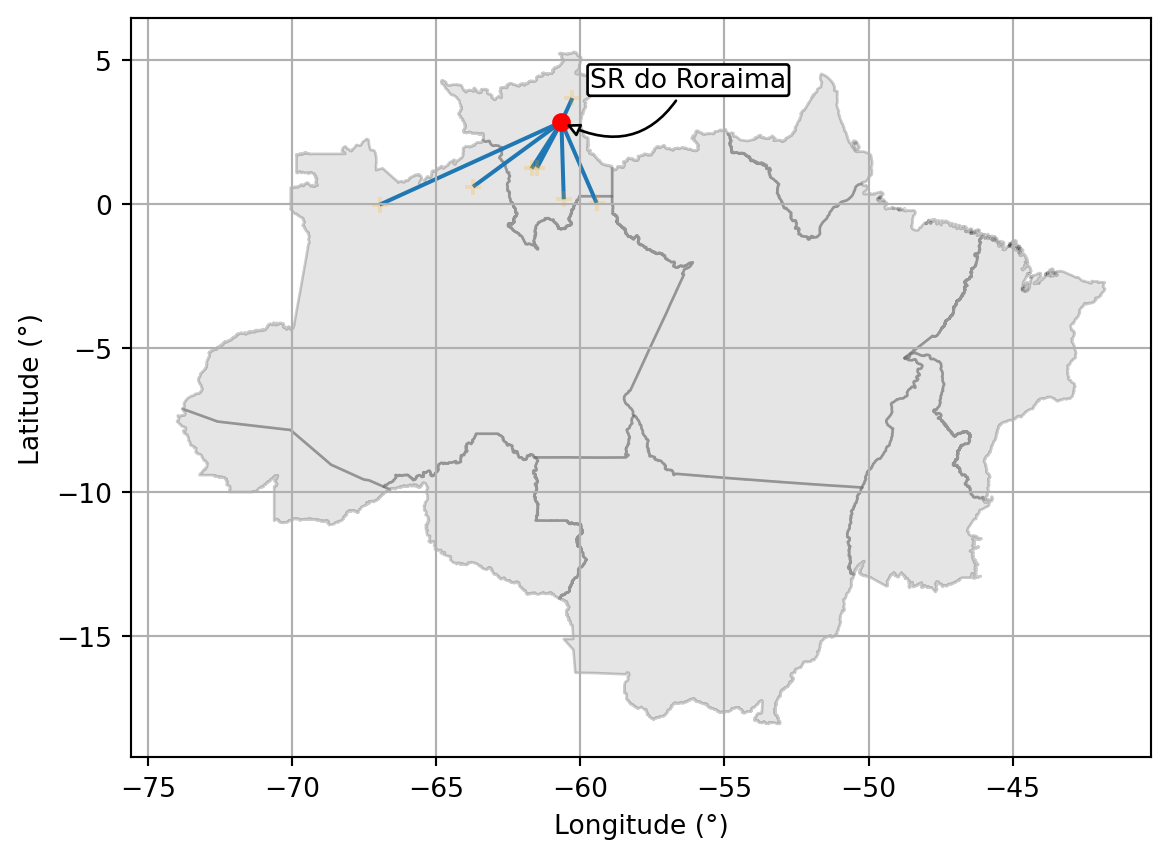
\includegraphics{./9-sr_files/figure-pdf/cell-6-output-22.pdf}

\hypertarget{distuxe2ncias-muxe9dias-e-muxe1ximas-das-glebas-em-relauxe7uxe3o-uxe0-sua-superintenduxeancia-regional-do-incra-recalculada.}{%
\subsection{Distâncias médias e máximas das glebas em relação à sua
Superintendência Regional do INCRA
recalculada.}\label{distuxe2ncias-muxe9dias-e-muxe1ximas-das-glebas-em-relauxe7uxe3o-uxe0-sua-superintenduxeancia-regional-do-incra-recalculada.}}

\n  

\n    

\n      

Superintendência

\n      

Distância Máxima (km)

\n      

Distância Média (km)

\n    

\n  

\n  

\n    

\n      

Acre

\n      

794

\n      

248

\n    

\n    

\n      

Amapá

\n      

434

\n      

228

\n    

\n    

\n      

Amazonas

\n      

657

\n      

187

\n    

\n    

\n      

Maranhão

\n      

333

\n      

206

\n    

\n    

\n      

Mato Grosso

\n      

729

\n      

282

\n    

\n    

\n      

Pará - Belém

\n      

283

\n      

140

\n    

\n    

\n      

Pará - Marabá

\n      

394

\n      

167

\n    

\n    

\n      

Pará - Santarém

\n      

709

\n      

217

\n    

\n    

\n      

Rondônia

\n      

572

\n      

249

\n    

\n    

\n      

Roraima

\n      

771

\n      

334

\n    

\n    

\n      

Tocantins

\n      

650

\n      

182

\n    

\n  

\n

\bookmarksetup{startatroot}

\hypertarget{situauxe7uxe3o-da-gleba.}{%
\chapter{Situação da gleba.}\label{situauxe7uxe3o-da-gleba.}}

Esta variável não possui informações que a descrevam de forma a
viabilizar sua utilização neste estudo.

As informações da situação das glebas estão classificadas com as
seguintes categorias:

\begin{itemize}
\tightlist
\item
  Sem informações
\item
  Certificada
\item
  Arrecadada
\item
  Titulação
\item
  Registrada
\item
  Aprovação Fiscal
\end{itemize}

\bookmarksetup{startatroot}

\hypertarget{glebas-com-assentimento-pruxe9vio-do-concelho-de-defesa-nacional---cdn.-1}{%
\chapter{Glebas com Assentimento prévio do Concelho de Defesa Nacional -
CDN.}\label{glebas-com-assentimento-pruxe9vio-do-concelho-de-defesa-nacional---cdn.-1}}

A Lei Nº 6.634, de 2 de maio de 1979, dispõe sobre a Faixa de Fronteira,
altera o Decreto-lei nº 1.135, de 3 de dezembro de 1970, e dá outras
providências.

\begin{quote}
Art. 1º. - É considerada área indispensável à Segurança Nacional a faixa
interna de 150 Km (cento e cinqüenta quilômetros) de largura, paralela à
linha divisória terrestre do território nacional, que será designada
como Faixa de Fronteira. Art. 2º. - Salvo com o assentimento prévio do
Conselho de Segurança Nacional, será vedada, na Faixa de Fronteira, a
prática dos atos referentes a:

I - alienação e concessão de terras públicas, abertura de vias de
transporte e instalação de meios de comunicação destinados à exploração
de serviços de radiodifusão de sons ou radiodifusão de sons e imagens;

II - Construção de pontes, estradas internacionais e campos de pouso;

III - estabelecimento ou exploração de indústrias que interessem à
Segurança Nacional, assim relacionadas em decreto do Poder Executivo.

IV - instalação de empresas que se dedicarem às seguintes atividades:

\begin{enumerate}
\def\labelenumi{\alph{enumi})}
\item
  pesquisa, lavra, exploração e aproveitamento de recursos minerais,
  salvo aqueles de imediata aplicação na construção civil, assim
  classificados no Código de Mineração;
\item
  colonização e loteamento rurais;
\end{enumerate}

V - transações com imóvel rural, que impliquem a obtenção, por
estrangeiro, do domínio, da posse ou de qualquer direito real sobre o
imóvel;

VI - participação, a qualquer título, de estrangeiro, pessoa natural ou
jurídica, em pessoa jurídica que seja titular de direito real sobre
imóvel rural;
\end{quote}

\hypertarget{glebas-federais-na-faixa-de-fronteira.}{%
\section{Glebas Federais na Faixa de
Fronteira.}\label{glebas-federais-na-faixa-de-fronteira.}}

\hypertarget{mapa-de-glebas-federais-na-faixa-de-fronteira-por-unidade-da-federauxe7uxe3o.}{%
\subsection{Mapa de glebas federais na faixa de fronteira por unidade da
federação.}\label{mapa-de-glebas-federais-na-faixa-de-fronteira-por-unidade-da-federauxe7uxe3o.}}

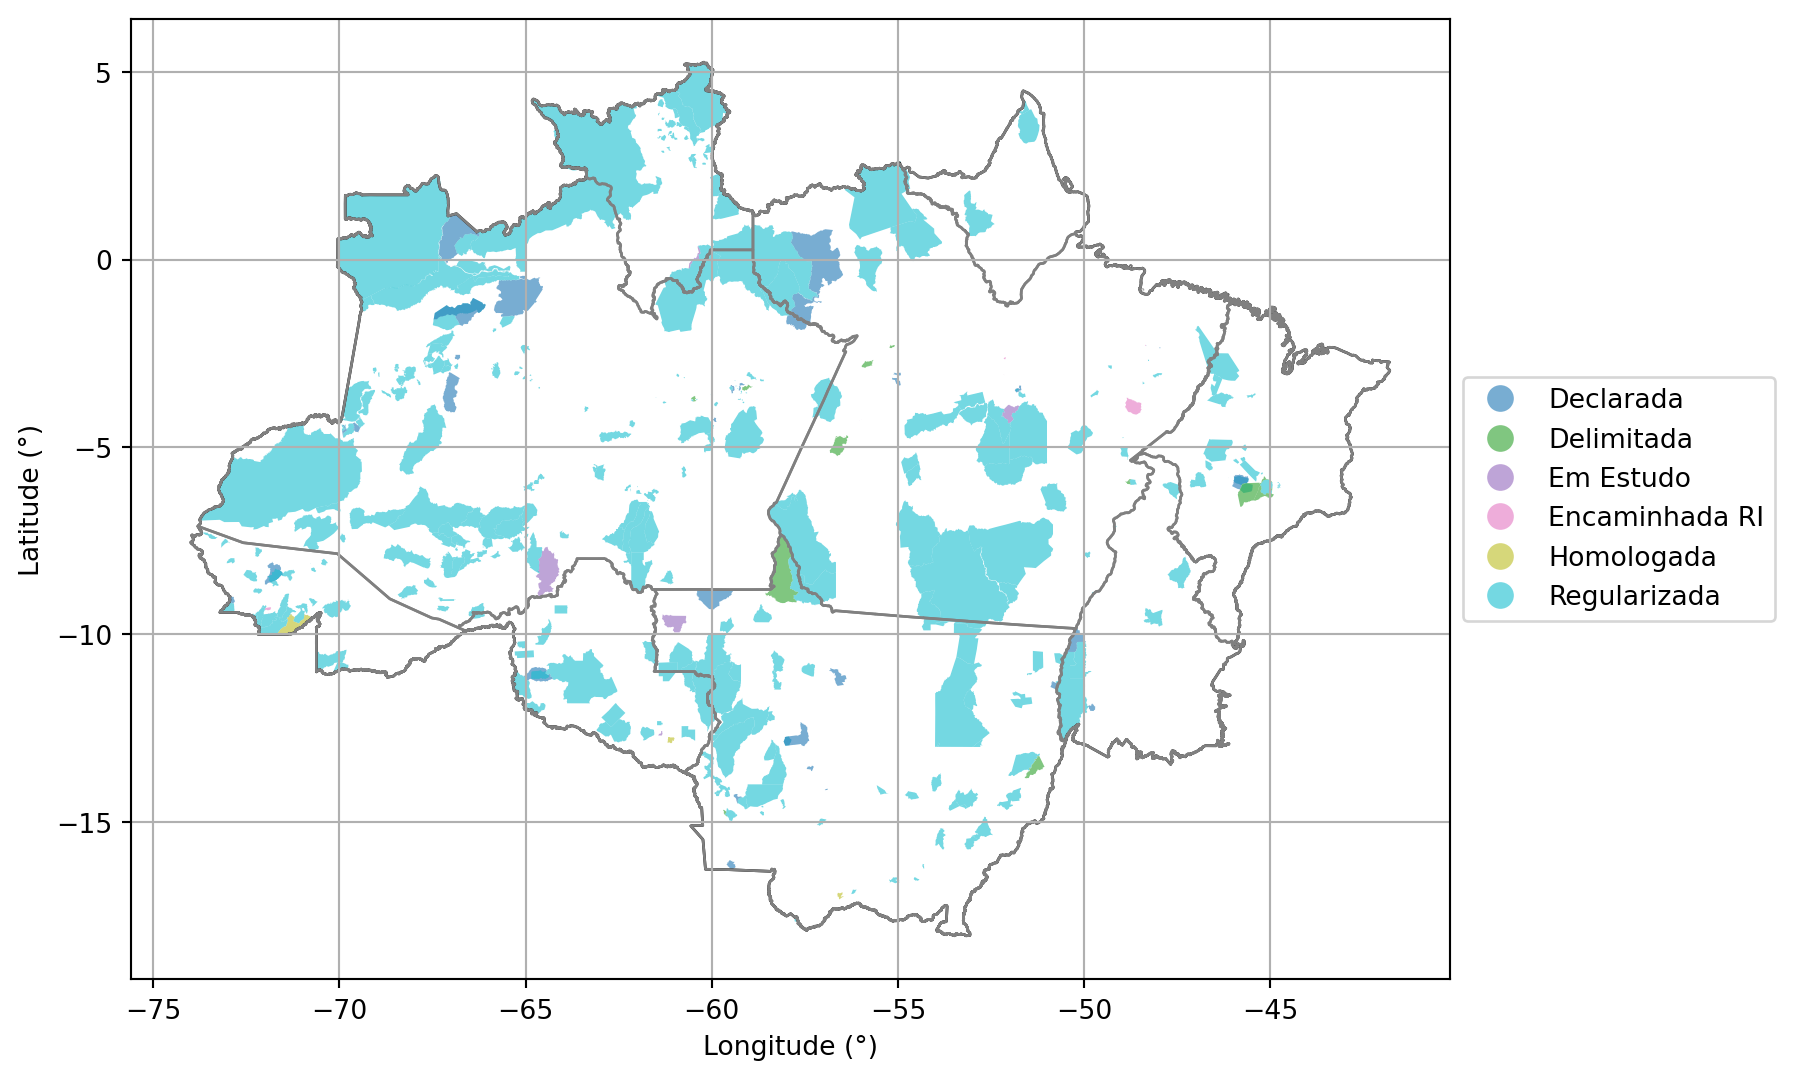
\includegraphics{./11-assentimento_files/figure-pdf/cell-2-output-1.pdf}

\hypertarget{tabela-de-glebas-federais-na-faixa-de-fronteira-por-unidade-da-federauxe7uxe3o}{%
\subsection{Tabela de glebas federais na faixa de fronteira por unidade
da
federação}\label{tabela-de-glebas-federais-na-faixa-de-fronteira-por-unidade-da-federauxe7uxe3o}}

\n  

\n    

\n      

UF

\n      

Quantidade

\n    

\n  

\n  

\n    

\n      

Acre

\n      

69

\n    

\n    

\n      

Amapá

\n      

12

\n    

\n    

\n      

Amazonas

\n      

67

\n    

\n    

\n      

Mato Grosso

\n      

146

\n    

\n    

\n      

Raraima

\n      

1

\n    

\n    

\n      

Rondônia

\n      

45

\n    

\n  

\n

\hypertarget{glebas-com-assentimento-pruxe9vio-por-superintenduxeancia.}{%
\section{Glebas com assentimento prévio por
Superintendência.}\label{glebas-com-assentimento-pruxe9vio-por-superintenduxeancia.}}

\hypertarget{mapa-de-glebas-federais-com-assentimento.}{%
\subsection{Mapa de glebas federais com
assentimento.}\label{mapa-de-glebas-federais-com-assentimento.}}

\includegraphics{./11-assentimento_files/figure-pdf/cell-4-output-1.pdf}

\hypertarget{tabela-de-glebas-federais-com-assentimento}{%
\subsection{Tabela de glebas federais com
assentimento}\label{tabela-de-glebas-federais-com-assentimento}}

\n  

\n    

\n      

UF

\n      

Quantidade

\n    

\n  

\n  

\n    

\n      

Acre

\n      

5

\n    

\n    

\n      

Amazonas

\n      

8

\n    

\n    

\n      

Mato Grosso

\n      

14

\n    

\n    

\n      

Rondônia

\n      

17

\n    

\n  

\n

\bookmarksetup{startatroot}

\hypertarget{sistema-nacional-de-cadastro-rural---sncr.}{%
\chapter{Sistema Nacional de Cadastro Rural -
SNCR.}\label{sistema-nacional-de-cadastro-rural---sncr.}}

\hypertarget{mapas-de-localizauxe7uxe3o-das-glebas-com-cuxf3digo-no-sistema-nacional-de-cadsatro-rural---sncr.}{%
\section{Mapas de localização das glebas com código no Sistema Nacional
de Cadsatro Rural -
SNCR.}\label{mapas-de-localizauxe7uxe3o-das-glebas-com-cuxf3digo-no-sistema-nacional-de-cadsatro-rural---sncr.}}

Os mapas abaixo mostram a distribuição das gelbas federais com cadastro
no SNCR por Superintendência Regional.

\hypertarget{superintenduxeancia-regional-do-acre.-2}{%
\subsection{Superintendência Regional do
Acre.}\label{superintenduxeancia-regional-do-acre.-2}}

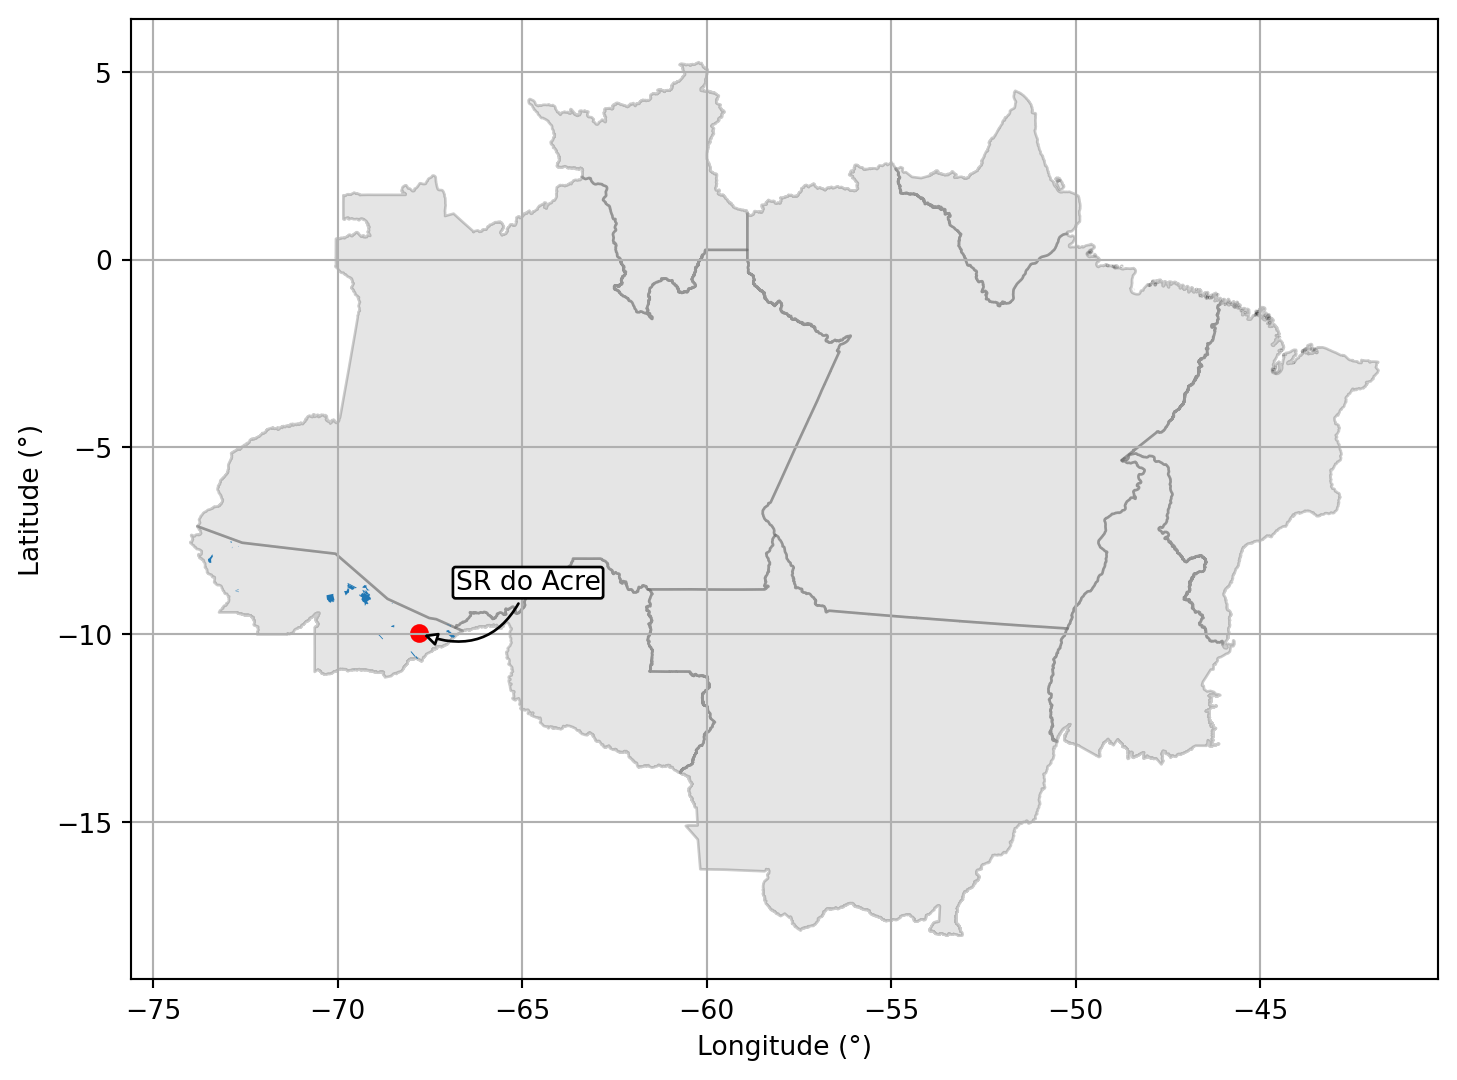
\includegraphics{./12-sncr_files/figure-pdf/cell-3-output-2.pdf}

\hypertarget{superintenduxeancia-regional-do-amapuxe1.-2}{%
\subsection{Superintendência Regional do
Amapá.}\label{superintenduxeancia-regional-do-amapuxe1.-2}}

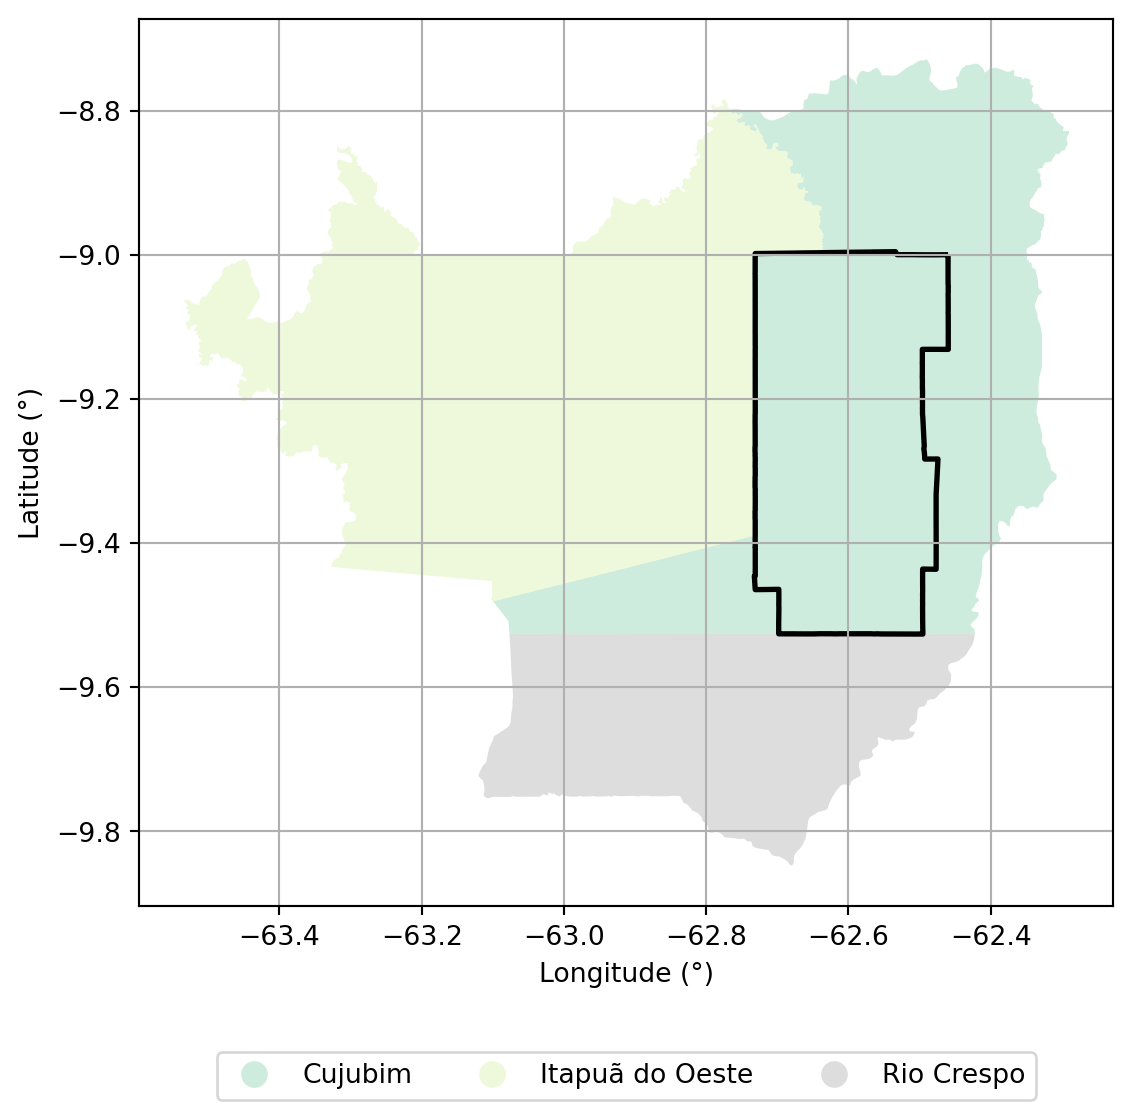
\includegraphics{./12-sncr_files/figure-pdf/cell-3-output-4.pdf}

\hypertarget{superintenduxeancia-regional-do-amazonas.-2}{%
\subsection{Superintendência Regional do
Amazonas.}\label{superintenduxeancia-regional-do-amazonas.-2}}

\includegraphics{./12-sncr_files/figure-pdf/cell-3-output-6.pdf}

\hypertarget{superintenduxeancia-regional-do-maranhuxe3o.-2}{%
\subsection{Superintendência Regional do
Maranhão.}\label{superintenduxeancia-regional-do-maranhuxe3o.-2}}

\includegraphics{./12-sncr_files/figure-pdf/cell-3-output-8.pdf}

\hypertarget{superintenduxeancia-regional-do-mato-grosso.-2}{%
\subsection{Superintendência Regional do Mato
Grosso.}\label{superintenduxeancia-regional-do-mato-grosso.-2}}

\includegraphics{./12-sncr_files/figure-pdf/cell-3-output-10.pdf}

\hypertarget{superintenduxeancia-regional-do-paruxe1---beluxe9m.-2}{%
\subsection{Superintendência Regional do Pará -
Belém.}\label{superintenduxeancia-regional-do-paruxe1---beluxe9m.-2}}

\includegraphics{./12-sncr_files/figure-pdf/cell-3-output-12.pdf}

\hypertarget{superintenduxeancia-regional-do-paruxe1---santaruxe9m.-2}{%
\subsection{Superintendência Regional do Pará -
Santarém.}\label{superintenduxeancia-regional-do-paruxe1---santaruxe9m.-2}}

\includegraphics{./12-sncr_files/figure-pdf/cell-3-output-14.pdf}

\hypertarget{superintenduxeancia-regional-do-paruxe1---marabuxe1.-2}{%
\subsection{Superintendência Regional do Pará -
Marabá.}\label{superintenduxeancia-regional-do-paruxe1---marabuxe1.-2}}

\includegraphics{./12-sncr_files/figure-pdf/cell-3-output-16.pdf}

\hypertarget{superintenduxeancia-regional-do-ronduxf4nia.-2}{%
\subsection{Superintendência Regional do
Rondônia.}\label{superintenduxeancia-regional-do-ronduxf4nia.-2}}

\includegraphics{./12-sncr_files/figure-pdf/cell-3-output-18.pdf}

\hypertarget{superintenduxeancia-regional-do-tocantins.-2}{%
\subsection{Superintendência Regional do
Tocantins.}\label{superintenduxeancia-regional-do-tocantins.-2}}

\includegraphics{./12-sncr_files/figure-pdf/cell-3-output-20.pdf}

\hypertarget{superintenduxeancia-regional-do-roraima.-2}{%
\subsection{Superintendência Regional do
Roraima.}\label{superintenduxeancia-regional-do-roraima.-2}}

\begin{verbatim}
/home/obt/.local/lib/python3.10/site-packages/geopandas/plotting.py:693: UserWarning:

The GeoDataFrame you are attempting to plot is empty. Nothing has been displayed.
\end{verbatim}

\includegraphics{./12-sncr_files/figure-pdf/cell-3-output-23.pdf}

\hypertarget{contagem-de-glebas-com-cadastro-no-sncr-por-superintenduxeancia-regional.}{%
\subsection{Contagem de Glebas com cadastro no SNCR por Superintendência
Regional.}\label{contagem-de-glebas-com-cadastro-no-sncr-por-superintenduxeancia-regional.}}

\n  

\n    

\n      

Superintendência

\n      

Qt. SNCR

\n      

Total

\n      

Perc. Cadastrado

\n    

\n  

\n  

\n    

\n      

Acre

\n      

31

\n      

81

\n      

38.27

\n    

\n    

\n      

Amapá

\n      

26

\n      

31

\n      

83.87

\n    

\n    

\n      

Amazonas

\n      

161

\n      

257

\n      

62.65

\n    

\n    

\n      

Maranhão

\n      

94

\n      

113

\n      

83.19

\n    

\n    

\n      

Mato Grosso

\n      

356

\n      

583

\n      

61.06

\n    

\n    

\n      

Pará - Belém

\n      

97

\n      

124

\n      

78.23

\n    

\n    

\n      

Pará - Marabá

\n      

118

\n      

188

\n      

62.77

\n    

\n    

\n      

Pará - Santarém

\n      

67

\n      

98

\n      

68.37

\n    

\n    

\n      

Rondônia

\n      

58

\n      

79

\n      

73.42

\n    

\n    

\n      

Roraima

\n      

0

\n      

3

\n      

0.00

\n    

\n    

\n      

Tocantins

\n      

62

\n      

544

\n      

11.40

\n    

\n  

\n

\bookmarksetup{startatroot}

\hypertarget{terras-induxedgenas.}{%
\chapter{Terras Indígenas.}\label{terras-induxedgenas.}}

\textbf{Terra Indígena (TI)} é uma porção dentro do território nacional,
habitada por uma ou mais comunidades indígenas, a qual após regular
processo administrativo, respeitado o devido processo legal, de
demarcação e homologação por Decreto Presidencial, é levado à registro
imobiliário como propriedade da União (artigo 20, XI, da CF/88),
perfectibilizando a área formalmente como de usufruto indígena. Assim
sendo, se trata de um bem de uso especial da União, afetado
administrativamente por uma finalidade pública.

Nos termos da legislação vigente (CF/88, Lei 6001/73 -- Estatuto do
Índio, Decreto n.º 1775/96), as terras indígenas podem ser classificadas
nas seguintes modalidades:

\textbf{Terras Indígenas Tradicionalmente Ocupadas:} São as terras
habitadas pelos indígenas em caráter permanente, utilizadas para
atividades produtivas, culturais, bem-estar e reprodução física, segundo
seus usos, costumes e tradições.

Para que seja considerada Terra Indígena, é necessário seguir
procedimento administrativo específico, no qual se observa o devido
processo legal como dito anteriormente, sendo que tal procedimento está
dividido por fases. Reservas Indígenas: São terras doadas por terceiros,
adquiridas ou desapropriadas pela União, que se destinam à posse
permanente dos indígenas. São terras que também pertencem ao patrimônio
da União, mas que não se confundem com as terras de ocupação
tradicional.

\textbf{Terras Dominiais:} São as terras de propriedade das comunidades
indígenas, havidas por qualquer das formas de aquisição do domínio, nos
termos da legislação civil.

\hypertarget{quantificauxe7uxe3o-das-terras-induxedgenas-por-unidade-da-federauxe7uxe3o}{%
\section{Quantificação das terras indígenas por unidade da
federação}\label{quantificauxe7uxe3o-das-terras-induxedgenas-por-unidade-da-federauxe7uxe3o}}

\includegraphics{./13-terra-indigena_files/figure-pdf/cell-2-output-1.pdf}

\hypertarget{mapa-de-terras-induxedgenas-por-unidade-da-federauxe7uxe3o}{%
\section{Mapa de terras indígenas por unidade da
federação}\label{mapa-de-terras-induxedgenas-por-unidade-da-federauxe7uxe3o}}

\includegraphics{./13-terra-indigena_files/figure-pdf/cell-3-output-1.pdf}

\hypertarget{quantida-de-uxe1rea-ocupada-com-terra-induxedgena---tocantins.}{%
\subsection{Quantida de área ocupada com Terra Indígena -
Tocantins.}\label{quantida-de-uxe1rea-ocupada-com-terra-induxedgena---tocantins.}}

\emph{25978.27km²}

\includegraphics{./13-terra-indigena_files/figure-pdf/cell-3-output-4.pdf}

\hypertarget{quantida-de-uxe1rea-ocupada-com-terra-induxedgena---ronduxf4nia.}{%
\subsection{Quantida de área ocupada com Terra Indígena -
Rondônia.}\label{quantida-de-uxe1rea-ocupada-com-terra-induxedgena---ronduxf4nia.}}

\emph{50650.06km²}

\includegraphics{./13-terra-indigena_files/figure-pdf/cell-3-output-7.pdf}

\hypertarget{quantida-de-uxe1rea-ocupada-com-terra-induxedgena---amazonas.}{%
\subsection{Quantida de área ocupada com Terra Indígena -
Amazonas.}\label{quantida-de-uxe1rea-ocupada-com-terra-induxedgena---amazonas.}}

\emph{467570.5km²}

\includegraphics{./13-terra-indigena_files/figure-pdf/cell-3-output-10.pdf}

\hypertarget{quantida-de-uxe1rea-ocupada-com-terra-induxedgena---acre.}{%
\subsection{Quantida de área ocupada com Terra Indígena -
Acre.}\label{quantida-de-uxe1rea-ocupada-com-terra-induxedgena---acre.}}

\emph{25509.4km²}

\includegraphics{./13-terra-indigena_files/figure-pdf/cell-3-output-13.pdf}

\hypertarget{quantida-de-uxe1rea-ocupada-com-terra-induxedgena---paruxe1.}{%
\subsection{Quantida de área ocupada com Terra Indígena -
Pará.}\label{quantida-de-uxe1rea-ocupada-com-terra-induxedgena---paruxe1.}}

\emph{309407.22km²}

\includegraphics{./13-terra-indigena_files/figure-pdf/cell-3-output-16.pdf}

\hypertarget{quantida-de-uxe1rea-ocupada-com-terra-induxedgena---mato-grosso.}{%
\subsection{Quantida de área ocupada com Terra Indígena - Mato
Grosso.}\label{quantida-de-uxe1rea-ocupada-com-terra-induxedgena---mato-grosso.}}

\emph{148058.27km²}

\includegraphics{./13-terra-indigena_files/figure-pdf/cell-3-output-19.pdf}

\hypertarget{quantida-de-uxe1rea-ocupada-com-terra-induxedgena---maranhuxe3o.}{%
\subsection{Quantida de área ocupada com Terra Indígena -
Maranhão.}\label{quantida-de-uxe1rea-ocupada-com-terra-induxedgena---maranhuxe3o.}}

\emph{23062.55km²}

\includegraphics{./13-terra-indigena_files/figure-pdf/cell-3-output-22.pdf}

\hypertarget{quantida-de-uxe1rea-ocupada-com-terra-induxedgena---amapuxe1.}{%
\subsection{Quantida de área ocupada com Terra Indígena -
Amapá.}\label{quantida-de-uxe1rea-ocupada-com-terra-induxedgena---amapuxe1.}}

\emph{11841.39km²}

\includegraphics{./13-terra-indigena_files/figure-pdf/cell-3-output-25.pdf}

\hypertarget{quantida-de-uxe1rea-ocupada-com-terra-induxedgena---roraima.}{%
\subsection{Quantida de área ocupada com Terra Indígena -
Roraima.}\label{quantida-de-uxe1rea-ocupada-com-terra-induxedgena---roraima.}}

\emph{104198.96km²}

\bookmarksetup{startatroot}

\hypertarget{unidades-de-consrvauxe7uxe3o.}{%
\chapter{Unidades de Consrvação.}\label{unidades-de-consrvauxe7uxe3o.}}

\hypertarget{unidade-de-conservauxe7uxe3o}{%
\section{Unidade de Conservação}\label{unidade-de-conservauxe7uxe3o}}

Áreas naturais relevantes para o Brasil são conhecidas como Unidades de
Conservação e são protegidas por Lei. Objetivo é garantir a preservação
da biodiversidade

Viver em um meio ambiente ecologicamente equilibrado é um direito de
todo brasileiro, garantido na Constituição Federal. Há muito o ser
humano reconhece a necessidade de proteger áreas naturais com
características específicas, salvaguardando fauna, flora, rios e mares,
elementos que precisam coexistir para haver equilíbrio na natureza. No
Brasil, país considerado megabiodiverso, essas áreas são delimitadas,
denominadas Unidades de Conservação (UC) e reguladas por lei.

Todas as unidades de conservação são espaços territoriais, incluindo as
águas jurisdicionais, com características naturais relevantes, que têm
como objetivo a conservação da natureza. Cada uma delas recebe uma
classificação diferente de acordo com suas características e objetivos a
serem atingidos.

Segundo o secretário de Ecoturismo do Ministério do Meio Ambiente (MMA),
André Germanos, cada UC recebe uma denominação diferente, de acordo com
seu nível de proteção exercida. ``Temos locais, biomas, regiões que
precisam ser preservadas por conta de alguma peculiaridade. Algumas
delas, por exemplo, são protegidas simplesmente porque têm uma beleza
cênica excepcional'', explica o secretário. ``Se por um lado temos a
beleza cênica, temos do outro a proteção ambiental de fato, que é a
preocupação com a fauna e flora. Elas podem ser destinadas à exploração
sustentável de recursos naturais, preservação total do ecossistema,
realização de pesquisas, visitação para promover a educação ambiental,
entre outras.''

A Lei nº 9.985, de 2000, instituiu o Sistema Nacional de Unidades de
Conservação (SNUC), que definiu a UC como um espaço territorial e seus
recursos ambientais, incluindo as águas jurisdicionais, com
características naturais relevantes. O SNUC também separou as áreas em
dois tipos: Unidades de Proteção Integral e Unidades de Uso Sustentável.
A primeira é subdividida em cinco categorias que possuem normas bastante
restritas e são mais voltadas para a pesquisa e conservação da
biodiversidade. Já as sete categorias de Unidades de Uso Sustentável são
mais voltadas para visitação e atividades educativas e uso sustentável
de seus recursos.

As Unidades de Proteção Integral são unidades de conservação de
fundamental importância para a preservação de ecossistemas,
proporcionado pesquisas científicas, manejo e educação ambiental na
busca pela conservação do meio ambiente. Elas são divididas em Unidades
de Proteção Integral e de Uso Sustentável. Fazem parte da primeira
categoria Estação Ecológica, Reserva Biológica, Parque Nacional,
Monumento Natural e Refúgio da Vida Silvestre. A segunda categoria
abrange Área de Proteção Ambiental, Floresta Nacional, Área de Relevante
Interesse Ecológico, Reserva Extrativista, Reserva da Fauna, Reserva
Extrativista, Reserva de Desenvolvimento Sustentável e Reserva
Particular do Patrimônio Natural.

Zoneamento -- Ainda que as Unidades de Uso Sustentável aliem a
preservação ambiental à exploração sustentável dos recursos naturais
cada pedacinho das UCs recebe uma denominação diferente. É o chamado
zoneamento, um processo que determina que usos serão dados às regiões
que ficam dentro das áreas protegidas, como explica Ugo Vercillo,
analista ambiental da Coordenação de Ações Integradas para Conservação
de Espécies do Instituto Chico Mendes de Conservação da Biodiversidade
(ICMBio), órgão ligado ao MMA e responsável pelas unidades de
conservação.

``Depois que se delimita a área de conservação, outros zoneamentos são
delimitados dentro dessa área protegida'', explica o biólogo. ``Essa
zona pode ser uma área intangível, ou seja, onde ninguém tem acesso, ou
pode ser uma área de uso múltiplo. Cada uma dessas áreas dentro de uma
UC tem aptidões diferentes.''

O zoneamento é definido pelo Plano de Manejo, que também inclui medidas
para promover a integração da UC à vida econômica e social das
comunidades vizinhas, o que é essencial para que implementação da
unidade seja mais eficiente.

fonte:\href{https://antigo.mma.gov.br/informma/item/15713-o-que-s\%C3\%A3o-as-unidades-de-conserva\%C3\%A7\%C3\%A3o.html}{Ministério
do Meio Ambiente}

\hypertarget{quantificauxe7uxe3o-das-unidades-de-conservauxe7uxe3o}{%
\subsection{Quantificação das Unidades de
Conservação}\label{quantificauxe7uxe3o-das-unidades-de-conservauxe7uxe3o}}

\includegraphics{./14-unidade-conservacao_files/figure-pdf/cell-3-output-1.pdf}

\hypertarget{unidade-de-conservauxe7uxe3o-por-categoria}{%
\subsection{Unidade de Conservação por
Categoria}\label{unidade-de-conservauxe7uxe3o-por-categoria}}

\n  

\n    

\n      

Categoria da Unidade de Conservação

\n      

Quantidade

\n      

Área (km²)

\n    

\n  

\n  

\n    

\n      

Estação Ecológica

\n      

19

\n      

114390.7597

\n    

\n    

\n      

Floresta

\n      

56

\n      

306729.0213

\n    

\n    

\n      

Monumento Natural

\n      

5

\n      

347.1177

\n    

\n    

\n      

Parque

\n      

81

\n      

299215.2247

\n    

\n    

\n      

Refúgio de Vida Silvestre

\n      

6

\n      

471.2235

\n    

\n    

\n      

Reserva Biológica

\n      

16

\n      

52965.8835

\n    

\n    

\n      

Reserva Extrativista

\n      

81

\n      

152665.4854

\n    

\n    

\n      

Reserva Particular do Patrimônio Natural

\n      

20

\n      

284.6641

\n    

\n    

\n      

Reserva de Desenvolvimento Sustentável

\n      

26

\n      

134330.2494

\n    

\n    

\n      

Área de Proteção Ambiental

\n      

57

\n      

285467.6319

\n    

\n    

\n      

Área de Relevante Interesse Ecológico

\n      

6

\n      

445.9002

\n    

\n  

\n

\hypertarget{unidade-de-conservauxe7uxe3o-por-estado}{%
\subsection{Unidade de Conservação por
estado}\label{unidade-de-conservauxe7uxe3o-por-estado}}

\n  

\n    

\n      

Categoria da Unidade de Conservação

\n      

Quantidade

\n      

Área (km²)

\n    

\n  

\n  

\n    

\n      

Estação Ecológica

\n      

19

\n      

114390.7597

\n    

\n    

\n      

Floresta

\n      

56

\n      

306729.0213

\n    

\n    

\n      

Monumento Natural

\n      

5

\n      

347.1177

\n    

\n    

\n      

Parque

\n      

81

\n      

299215.2247

\n    

\n    

\n      

Refúgio de Vida Silvestre

\n      

6

\n      

471.2235

\n    

\n    

\n      

Reserva Biológica

\n      

16

\n      

52965.8835

\n    

\n    

\n      

Reserva Extrativista

\n      

81

\n      

152665.4854

\n    

\n    

\n      

Reserva Particular do Patrimônio Natural

\n      

20

\n      

284.6641

\n    

\n    

\n      

Reserva de Desenvolvimento Sustentável

\n      

26

\n      

134330.2494

\n    

\n    

\n      

Área de Proteção Ambiental

\n      

57

\n      

285467.6319

\n    

\n    

\n      

Área de Relevante Interesse Ecológico

\n      

6

\n      

445.9002

\n    

\n  

\n

\hypertarget{cadastro-nacional-de-florestas-puxfablicas-cnfp}{%
\section{Cadastro Nacional de Florestas Públicas
(CNFP)}\label{cadastro-nacional-de-florestas-puxfablicas-cnfp}}

O Cadastro Nacional de Florestas Públicas (CNFP) é um instrumento de
planejamento da gestão florestal, que reúne dados georreferenciados
sobre as florestas públicas brasileiras, de modo a oferecer aos gestores
públicos e à população em geral uma base confiável de mapas, imagens e
dados com informações relevantes para a gestão florestal. Os dados do
CNFP auxiliam os processos de destinação das florestas públicas para uso
comunitário, criação de unidades de conservação e realização de
concessões florestais. O Cadastro contribui para a transparência, a
participação social e unificação das informações sobre as florestas
públicas.

O CNFP é formado pelo Cadastro de Florestas Públicas da União, pelos
Cadastros de Florestas Públicas dos estados, Distrito Federal e
municípios e está em processo de interligação ao Sistema Nacional de
Cadastro Rural (SNCR) do Instituto Nacional de Colonização e Reforma
Agrária (INCRA).

O cadastramento das florestas públicas segue três etapas:

\begin{itemize}
\tightlist
\item
  Identificação - mapeamento das florestas localizadas em áreas
  públicas;
\item
  Delimitação- averbação (registro) do perímetro da floresta junto à
  matricula do imóvel público;
\item
  Demarcação - implantação de marcos topográficos e colocação de placas
  informativas no campo.
\end{itemize}

Existem três tipos de florestas públicas federais:

\begin{itemize}
\tightlist
\item
  Florestas Públicas do TIPO A (FPA) - São florestas que apresentam
  destinação e dominialidade específica como as Unidades de Conservação
  da Natureza, as Terras Indígenas, os Assentamentos Rurais Públicos, as
  áreas militares e outras formas de destinação previstas em lei. São
  destinadas à proteção e conservação do meio ambiente e uso de
  comunidades tradicionais
\item
  Florestas Públicas do TIPO B (FPB) - São as florestas localizadas em
  áreas arrecadadas pelo Poder Público, mas que ainda não foram
  destinadas.
\item
  Florestas Públicas do TIPO C (FPC) - São as florestas localizadas em
  áreas de dominialidade indefinida, comumente chamadas de terras
  devolutas.
\end{itemize}

fonte:
\href{https://www.gov.br/agricultura/pt-br/assuntos/servico-florestal-brasileiro/cadastro-nacional-de-florestas-publicas}{Serviço
Florestal Brasileiro}

\hypertarget{quantificauxe7uxe3o-das-florestas-publicas-por-tipo}{%
\subsection{Quantificação das florestas publicas por
tipo}\label{quantificauxe7uxe3o-das-florestas-publicas-por-tipo}}

\includegraphics{./14-unidade-conservacao_files/figure-pdf/cell-6-output-1.pdf}

\n  

\n    

\n      

Tipo de Floresta Publica

\n      

Área (ha)

\n    

\n  

\n  

\n    

\n      

TIPO A

\n      

235982649

\n    

\n    

\n      

TIPO B

\n      

62989475

\n    

\n  

\n

A denominação de florestas publicas parece abranger integralmentes as
poligonais já classificadas em outras atividades tais como áreas de
assentamentos federais, assim, a denominação que pode remeter a uma área
de vegetação nativa não é a realizada das poligonais existentes na base
de dados.

As áreas mensuradas como florestas publicas abrangem divérsos uso do
solo distintos de vegetação nativa, levando à conclusões equivocadas
quando do uso da totalização de área.

Seguindo a definição do Serviço Florestal Brasileiro, as florestas
publicas do \emph{Tipo A - lorestas que apresentam destinação e
dominialidade específica}, somariam 235.982.649 de hectares e as do
\emph{Tipo B - São as florestas localizadas em áreas arrecadadas pelo
Poder Público, mas que ainda não foram destinadas} somariam 62.989.475
de hectares. Porém esse número não corresponde à área ocupada por
vergetação nativa nos respectivos polígonos.

\bookmarksetup{startatroot}

\hypertarget{anuxe1lise-dos-municuxedpios-na-uxe1rea-de-estudo.}{%
\chapter{Análise dos Municípios na área de
estudo.}\label{anuxe1lise-dos-municuxedpios-na-uxe1rea-de-estudo.}}

A área de estudo contempla 808 municípios nos nas 09 unidades da
federação. Destes, 512 possuem áreas de glebas publicas federais em seu
território.

\hypertarget{mapa-dos-municuxedpios-na-uxe1rea-de-estudo.}{%
\section{Mapa dos Municípios na área de
estudo.}\label{mapa-dos-municuxedpios-na-uxe1rea-de-estudo.}}

\includegraphics{./15-municipios_files/figure-pdf/cell-3-output-1.pdf}

\hypertarget{tabela-dos-municuxedpios-com-glebas-publicas-federais.}{%
\section{Tabela dos Municípios com glebas publicas
federais.}\label{tabela-dos-municuxedpios-com-glebas-publicas-federais.}}

\n  

\n    

\n      

Estado

\n      

Código do Município

\n      

Nome do Município

\n    

\n  

\n  

\n    

\n      

Acre

\n      

1200427

\n      

Rodrigues Alves

\n    

\n    

\n      

Acre

\n      

1200708

\n      

Xapuri

\n    

\n    

\n      

Acre

\n      

1200609

\n      

Tarauacá

\n    

\n    

\n      

Acre

\n      

1200500

\n      

Sena Madureira

\n    

\n    

\n      

Acre

\n      

1200450

\n      

Senador Guiomard

\n    

\n    

\n      

Acre

\n      

1200013

\n      

Acrelândia

\n    

\n    

\n      

Acre

\n      

1200054

\n      

Assis Brasil

\n    

\n    

\n      

Acre

\n      

1200435

\n      

Santa Rosa do Purus

\n    

\n    

\n      

Acre

\n      

1200807

\n      

Porto Acre

\n    

\n    

\n      

Acre

\n      

1200104

\n      

Brasiléia

\n    

\n    

\n      

Acre

\n      

1200179

\n      

Capixaba

\n    

\n    

\n      

Acre

\n      

1200203

\n      

Cruzeiro do Sul

\n    

\n    

\n      

Acre

\n      

1200252

\n      

Epitaciolândia

\n    

\n    

\n      

Acre

\n      

1200302

\n      

Feijó

\n    

\n    

\n      

Acre

\n      

1200401

\n      

Rio Branco

\n    

\n    

\n      

Acre

\n      

1200385

\n      

Plácido de Castro

\n    

\n    

\n      

Acre

\n      

1200336

\n      

Mâncio Lima

\n    

\n    

\n      

Acre

\n      

1200138

\n      

Bujari

\n    

\n    

\n      

Acre

\n      

1200351

\n      

Marechal Thaumaturgo

\n    

\n    

\n      

Acre

\n      

1200344

\n      

Manoel Urbano

\n    

\n    

\n      

Amapá

\n      

1600204

\n      

Calçoene

\n    

\n    

\n      

Amapá

\n      

1600279

\n      

Laranjal do Jari

\n    

\n    

\n      

Amapá

\n      

1600402

\n      

Mazagão

\n    

\n    

\n      

Amapá

\n      

1600253

\n      

Itaubal

\n    

\n    

\n      

Amapá

\n      

1600501

\n      

Oiapoque

\n    

\n    

\n      

Amapá

\n      

1600238

\n      

Ferreira Gomes

\n    

\n    

\n      

Amapá

\n      

1600535

\n      

Porto Grande

\n    

\n    

\n      

Amapá

\n      

1600212

\n      

Cutias

\n    

\n    

\n      

Amapá

\n      

1600154

\n      

Pedra Branca do Amapari

\n    

\n    

\n      

Amapá

\n      

1600105

\n      

Amapá

\n    

\n    

\n      

Amapá

\n      

1600055

\n      

Serra do Navio

\n    

\n    

\n      

Amapá

\n      

1600550

\n      

Pracuúba

\n    

\n    

\n      

Amapá

\n      

1600600

\n      

Santana

\n    

\n    

\n      

Amapá

\n      

1600709

\n      

Tartarugalzinho

\n    

\n    

\n      

Amapá

\n      

1600303

\n      

Macapá

\n    

\n    

\n      

Amazonas

\n      

1303403

\n      

Parintins

\n    

\n    

\n      

Amazonas

\n      

1303809

\n      

São Gabriel da Cachoeira

\n    

\n    

\n      

Amazonas

\n      

1303700

\n      

Santo Antônio do Içá

\n    

\n    

\n      

Amazonas

\n      

1304005

\n      

Silves

\n    

\n    

\n      

Amazonas

\n      

1300086

\n      

Anamã

\n    

\n    

\n      

Amazonas

\n      

1300060

\n      

Amaturá

\n    

\n    

\n      

Amazonas

\n      

1303601

\n      

Santa Isabel do Rio Negro

\n    

\n    

\n      

Amazonas

\n      

1304104

\n      

Tapauá

\n    

\n    

\n      

Amazonas

\n      

1302702

\n      

Manicoré

\n    

\n    

\n      

Amazonas

\n      

1304062

\n      

Tabatinga

\n    

\n    

\n      

Amazonas

\n      

1303569

\n      

Rio Preto da Eva

\n    

\n    

\n      

Amazonas

\n      

1303502

\n      

Pauini

\n    

\n    

\n      

Amazonas

\n      

1302900

\n      

Maués

\n    

\n    

\n      

Amazonas

\n      

1303007

\n      

Nhamundá

\n    

\n    

\n      

Amazonas

\n      

1303106

\n      

Nova Olinda do Norte

\n    

\n    

\n      

Amazonas

\n      

1303536

\n      

Presidente Figueiredo

\n    

\n    

\n      

Amazonas

\n      

1303205

\n      

Novo Airão

\n    

\n    

\n      

Amazonas

\n      

1300102

\n      

Anori

\n    

\n    

\n      

Amazonas

\n      

1303304

\n      

Novo Aripuanã

\n    

\n    

\n      

Amazonas

\n      

1303908

\n      

São Paulo de Olivença

\n    

\n    

\n      

Amazonas

\n      

1304237

\n      

Tonantins

\n    

\n    

\n      

Amazonas

\n      

1302504

\n      

Manacapuru

\n    

\n    

\n      

Amazonas

\n      

1302553

\n      

Manaquiri

\n    

\n    

\n      

Amazonas

\n      

1304302

\n      

Urucará

\n    

\n    

\n      

Amazonas

\n      

1302405

\n      

Lábrea

\n    

\n    

\n      

Amazonas

\n      

1304401

\n      

Urucurituba

\n    

\n    

\n      

Amazonas

\n      

1302306

\n      

Jutaí

\n    

\n    

\n      

Amazonas

\n      

1302108

\n      

Japurá

\n    

\n    

\n      

Amazonas

\n      

1302009

\n      

Itapiranga

\n    

\n    

\n      

Amazonas

\n      

1301902

\n      

Itacoatiara

\n    

\n    

\n      

Amazonas

\n      

1301852

\n      

Iranduba

\n    

\n    

\n      

Amazonas

\n      

1301704

\n      

Humaitá

\n    

\n    

\n      

Amazonas

\n      

1301654

\n      

Guajará

\n    

\n    

\n      

Amazonas

\n      

1301308

\n      

Codajás

\n    

\n    

\n      

Amazonas

\n      

1301209

\n      

Coari

\n    

\n    

\n      

Amazonas

\n      

1301159

\n      

Careiro da Várzea

\n    

\n    

\n      

Amazonas

\n      

1301100

\n      

Careiro

\n    

\n    

\n      

Amazonas

\n      

1300904

\n      

Canutama

\n    

\n    

\n      

Amazonas

\n      

1300839

\n      

Caapiranga

\n    

\n    

\n      

Amazonas

\n      

1300805

\n      

Borba

\n    

\n    

\n      

Amazonas

\n      

1300706

\n      

Boca do Acre

\n    

\n    

\n      

Amazonas

\n      

1302603

\n      

Manaus

\n    

\n    

\n      

Amazonas

\n      

1300680

\n      

Boa Vista do Ramos

\n    

\n    

\n      

Amazonas

\n      

1300631

\n      

Beruri

\n    

\n    

\n      

Amazonas

\n      

1300607

\n      

Benjamin Constant

\n    

\n    

\n      

Amazonas

\n      

1300508

\n      

Barreirinha

\n    

\n    

\n      

Amazonas

\n      

1300409

\n      

Barcelos

\n    

\n    

\n      

Amazonas

\n      

1300300

\n      

Autazes

\n    

\n    

\n      

Amazonas

\n      

1300144

\n      

Apuí

\n    

\n    

\n      

Amazonas

\n      

1300201

\n      

Atalaia do Norte

\n    

\n    

\n      

Amazonas

\n      

1303957

\n      

São Sebastião do Uatumã

\n    

\n    

\n      

Maranhão

\n      

2107803

\n      

Parnarama

\n    

\n    

\n      

Maranhão

\n      

2105427

\n      

Itinga do Maranhão

\n    

\n    

\n      

Maranhão

\n      

2111078

\n      

São João do Soter

\n    

\n    

\n      

Maranhão

\n      

2105476

\n      

Jenipapo dos Vieiras

\n    

\n    

\n      

Maranhão

\n      

2105500

\n      

João Lisboa

\n    

\n    

\n      

Maranhão

\n      

2110856

\n      

São Francisco do Brejão

\n    

\n    

\n      

Maranhão

\n      

2105609

\n      

Joselândia

\n    

\n    

\n      

Maranhão

\n      

2110039

\n      

Santa Luzia do Paruá

\n    

\n    

\n      

Maranhão

\n      

2105658

\n      

Junco do Maranhão

\n    

\n    

\n      

Maranhão

\n      

2101970

\n      

Boa Vista do Gurupi

\n    

\n    

\n      

Maranhão

\n      

2105708

\n      

Lago da Pedra

\n    

\n    

\n      

Maranhão

\n      

2102002

\n      

Bom Jardim

\n    

\n    

\n      

Maranhão

\n      

2105963

\n      

Lagoa Grande do Maranhão

\n    

\n    

\n      

Maranhão

\n      

2109908

\n      

Santa Inês

\n    

\n    

\n      

Maranhão

\n      

2102036

\n      

Bom Jesus das Selvas

\n    

\n    

\n      

Maranhão

\n      

2108405

\n      

Peri Mirim

\n    

\n    

\n      

Maranhão

\n      

2109809

\n      

Santa Helena

\n    

\n    

\n      

Maranhão

\n      

2109551

\n      

Ribamar Fiquene

\n    

\n    

\n      

Maranhão

\n      

2106326

\n      

Maracaçumé

\n    

\n    

\n      

Maranhão

\n      

2109502

\n      

Riachão

\n    

\n    

\n      

Maranhão

\n      

2106375

\n      

Maranhãozinho

\n    

\n    

\n      

Maranhão

\n      

2102358

\n      

Buritirana

\n    

\n    

\n      

Maranhão

\n      

2106904

\n      

Monção

\n    

\n    

\n      

Maranhão

\n      

2109239

\n      

Presidente Médici

\n    

\n    

\n      

Maranhão

\n      

2107001

\n      

Montes Altos

\n    

\n    

\n      

Maranhão

\n      

2108900

\n      

Poção de Pedras

\n    

\n    

\n      

Maranhão

\n      

2107357

\n      

Nova Olinda do Maranhão

\n    

\n    

\n      

Maranhão

\n      

2103158

\n      

Centro do Guilherme

\n    

\n    

\n      

Maranhão

\n      

2107407

\n      

Olho d\textquotesingle Água das Cunhãs

\n    

\n    

\n      

Maranhão

\n      

2108256

\n      

Pedro do Rosário

\n    

\n    

\n      

Maranhão

\n      

2108306

\n      

Penalva

\n    

\n    

\n      

Maranhão

\n      

2103000

\n      

Caxias

\n    

\n    

\n      

Maranhão

\n      

2101905

\n      

Bequimão

\n    

\n    

\n      

Maranhão

\n      

2105351

\n      

Itaipava do Grajaú

\n    

\n    

\n      

Maranhão

\n      

2111508

\n      

São Mateus do Maranhão

\n    

\n    

\n      

Maranhão

\n      

2100402

\n      

Altamira do Maranhão

\n    

\n    

\n      

Maranhão

\n      

2100055

\n      

Açailândia

\n    

\n    

\n      

Maranhão

\n      

2114007

\n      

Zé Doca

\n    

\n    

\n      

Maranhão

\n      

2113009

\n      

Vitorino Freire

\n    

\n    

\n      

Maranhão

\n      

2112852

\n      

Vila Nova dos Martírios

\n    

\n    

\n      

Maranhão

\n      

2111763

\n      

Senador La Rocque

\n    

\n    

\n      

Maranhão

\n      

2111748

\n      

Senador Alexandre Costa

\n    

\n    

\n      

Maranhão

\n      

2100600

\n      

Amarante do Maranhão

\n    

\n    

\n      

Maranhão

\n      

2103174

\n      

Centro Novo do Maranhão

\n    

\n    

\n      

Maranhão

\n      

2100873

\n      

Araguanã

\n    

\n    

\n      

Maranhão

\n      

2111722

\n      

Satubinha

\n    

\n    

\n      

Maranhão

\n      

2103257

\n      

Cidelândia

\n    

\n    

\n      

Maranhão

\n      

2111672

\n      

São Roberto

\n    

\n    

\n      

Maranhão

\n      

2105302

\n      

Imperatriz

\n    

\n    

\n      

Maranhão

\n      

2101202

\n      

Bacabal

\n    

\n    

\n      

Maranhão

\n      

2103752

\n      

Davinópolis

\n    

\n    

\n      

Maranhão

\n      

2108702

\n      

Pio XII

\n    

\n    

\n      

Maranhão

\n      

2101608

\n      

Barra do Corda

\n    

\n    

\n      

Maranhão

\n      

2104057

\n      

Estreito

\n    

\n    

\n      

Maranhão

\n      

2111631

\n      

São Raimundo do Doca Bezerra

\n    

\n    

\n      

Maranhão

\n      

2104206

\n      

Fortuna

\n    

\n    

\n      

Maranhão

\n      

2111532

\n      

São Pedro da Água Branca

\n    

\n    

\n      

Maranhão

\n      

2104404

\n      

Gonçalves Dias

\n    

\n    

\n      

Maranhão

\n      

2104552

\n      

Governador Edison Lobão

\n    

\n    

\n      

Maranhão

\n      

2104602

\n      

Governador Eugênio Barros

\n    

\n    

\n      

Maranhão

\n      

2105153

\n      

Igarapé do Meio

\n    

\n    

\n      

Maranhão

\n      

2104008

\n      

Esperantinópolis

\n    

\n    

\n      

Maranhão

\n      

2101772

\n      

Bela Vista do Maranhão

\n    

\n    

\n      

Maranhão

\n      

2104628

\n      

Governador Luiz Rocha

\n    

\n    

\n      

Maranhão

\n      

2104651

\n      

Governador Newton Bello

\n    

\n    

\n      

Maranhão

\n      

2104677

\n      

Governador Nunes Freire

\n    

\n    

\n      

Mato Grosso

\n      

5107008

\n      

Poxoréu

\n    

\n    

\n      

Mato Grosso

\n      

5107156

\n      

Reserva do Cabaçal

\n    

\n    

\n      

Mato Grosso

\n      

5107107

\n      

São José dos Quatro Marcos

\n    

\n    

\n      

Mato Grosso

\n      

5107040

\n      

Primavera do Leste

\n    

\n    

\n      

Mato Grosso

\n      

5107198

\n      

Ribeirãozinho

\n    

\n    

\n      

Mato Grosso

\n      

5107180

\n      

Ribeirão Cascalheira

\n    

\n    

\n      

Mato Grosso

\n      

5108352

\n      

Vale de São Domingos

\n    

\n    

\n      

Mato Grosso

\n      

5107305

\n      

São José do Rio Claro

\n    

\n    

\n      

Mato Grosso

\n      

5108204

\n      

Torixoréu

\n    

\n    

\n      

Mato Grosso

\n      

5108402

\n      

Várzea Grande

\n    

\n    

\n      

Mato Grosso

\n      

5108105

\n      

Tesouro

\n    

\n    

\n      

Mato Grosso

\n      

5108501

\n      

Vera

\n    

\n    

\n      

Mato Grosso

\n      

5108055

\n      

Terra Nova do Norte

\n    

\n    

\n      

Mato Grosso

\n      

5108808

\n      

Nova Guarita

\n    

\n    

\n      

Mato Grosso

\n      

5108857

\n      

Nova Marilândia

\n    

\n    

\n      

Mato Grosso

\n      

5108907

\n      

Nova Maringá

\n    

\n    

\n      

Mato Grosso

\n      

5107958

\n      

Tangará da Serra

\n    

\n    

\n      

Mato Grosso

\n      

5107925

\n      

Sorriso

\n    

\n    

\n      

Mato Grosso

\n      

5107909

\n      

Sinop

\n    

\n    

\n      

Mato Grosso

\n      

5107883

\n      

Serra Nova Dourada

\n    

\n    

\n      

Mato Grosso

\n      

5107875

\n      

Sapezal

\n    

\n    

\n      

Mato Grosso

\n      

5107859

\n      

São Félix do Araguaia

\n    

\n    

\n      

Mato Grosso

\n      

5107800

\n      

Santo Antônio do Leverger

\n    

\n    

\n      

Mato Grosso

\n      

5107792

\n      

Santo Antônio do Leste

\n    

\n    

\n      

Mato Grosso

\n      

5108303

\n      

União do Sul

\n    

\n    

\n      

Mato Grosso

\n      

5107750

\n      

Salto do Céu

\n    

\n    

\n      

Mato Grosso

\n      

5107701

\n      

Rosário Oeste

\n    

\n    

\n      

Mato Grosso

\n      

5107602

\n      

Rondonópolis

\n    

\n    

\n      

Mato Grosso

\n      

5107578

\n      

Rondolândia

\n    

\n    

\n      

Mato Grosso

\n      

5107404

\n      

São Pedro da Cipa

\n    

\n    

\n      

Mato Grosso

\n      

5107354

\n      

São José do Xingu

\n    

\n    

\n      

Mato Grosso

\n      

5107248

\n      

Santa Carmem

\n    

\n    

\n      

Mato Grosso

\n      

5107768

\n      

Santa Rita do Trivelato

\n    

\n    

\n      

Mato Grosso

\n      

5106109

\n      

Nossa Senhora do Livramento

\n    

\n    

\n      

Mato Grosso

\n      

5106828

\n      

Porto Esperidião

\n    

\n    

\n      

Mato Grosso

\n      

5103809

\n      

Figueirópolis D\textquotesingle Oeste

\n    

\n    

\n      

Mato Grosso

\n      

5103601

\n      

Dom Aquino

\n    

\n    

\n      

Mato Grosso

\n      

5103502

\n      

Diamantino

\n    

\n    

\n      

Mato Grosso

\n      

5103437

\n      

Curvelândia

\n    

\n    

\n      

Mato Grosso

\n      

5103403

\n      

Cuiabá

\n    

\n    

\n      

Mato Grosso

\n      

5103361

\n      

Conquista D\textquotesingle Oeste

\n    

\n    

\n      

Mato Grosso

\n      

5103353

\n      

Confresa

\n    

\n    

\n      

Mato Grosso

\n      

5103304

\n      

Comodoro

\n    

\n    

\n      

Mato Grosso

\n      

5103254

\n      

Colniza

\n    

\n    

\n      

Mato Grosso

\n      

5103205

\n      

Colíder

\n    

\n    

\n      

Mato Grosso

\n      

5103106

\n      

Cocalinho

\n    

\n    

\n      

Mato Grosso

\n      

5103056

\n      

Cláudia

\n    

\n    

\n      

Mato Grosso

\n      

5106851

\n      

Porto Estrela

\n    

\n    

\n      

Mato Grosso

\n      

5102793

\n      

Carlinda

\n    

\n    

\n      

Mato Grosso

\n      

5102694

\n      

Canabrava do Norte

\n    

\n    

\n      

Mato Grosso

\n      

5102686

\n      

Campos de Júlio

\n    

\n    

\n      

Mato Grosso

\n      

5102678

\n      

Campo Verde

\n    

\n    

\n      

Mato Grosso

\n      

5100102

\n      

Acorizal

\n    

\n    

\n      

Mato Grosso

\n      

5100201

\n      

Água Boa

\n    

\n    

\n      

Mato Grosso

\n      

5100250

\n      

Alta Floresta

\n    

\n    

\n      

Mato Grosso

\n      

5100508

\n      

Alto Paraguai

\n    

\n    

\n      

Mato Grosso

\n      

5100805

\n      

Apiacás

\n    

\n    

\n      

Mato Grosso

\n      

5101001

\n      

Araguaiana

\n    

\n    

\n      

Mato Grosso

\n      

5103908

\n      

General Carneiro

\n    

\n    

\n      

Mato Grosso

\n      

5101258

\n      

Araputanga

\n    

\n    

\n      

Mato Grosso

\n      

5101704

\n      

Barra do Bugres

\n    

\n    

\n      

Mato Grosso

\n      

5101803

\n      

Barra do Garças

\n    

\n    

\n      

Mato Grosso

\n      

5101852

\n      

Bom Jesus do Araguaia

\n    

\n    

\n      

Mato Grosso

\n      

5102504

\n      

Cáceres

\n    

\n    

\n      

Mato Grosso

\n      

5102603

\n      

Campinápolis

\n    

\n    

\n      

Mato Grosso

\n      

5102637

\n      

Campo Novo do Parecis

\n    

\n    

\n      

Mato Grosso

\n      

5101605

\n      

Barão de Melgaço

\n    

\n    

\n      

Mato Grosso

\n      

5103957

\n      

Glória D\textquotesingle Oeste

\n    

\n    

\n      

Mato Grosso

\n      

5103007

\n      

Chapada dos Guimarães

\n    

\n    

\n      

Mato Grosso

\n      

5104203

\n      

Guiratinga

\n    

\n    

\n      

Mato Grosso

\n      

5106208

\n      

Nova Brasilândia

\n    

\n    

\n      

Mato Grosso

\n      

5106216

\n      

Nova Canaã do Norte

\n    

\n    

\n      

Mato Grosso

\n      

5106224

\n      

Nova Mutum

\n    

\n    

\n      

Mato Grosso

\n      

5106232

\n      

Nova Olímpia

\n    

\n    

\n      

Mato Grosso

\n      

5106257

\n      

Nova Xavantina

\n    

\n    

\n      

Mato Grosso

\n      

5106265

\n      

Novo Mundo

\n    

\n    

\n      

Mato Grosso

\n      

5106190

\n      

Nova Santa Helena

\n    

\n    

\n      

Mato Grosso

\n      

5106281

\n      

Novo São Joaquim

\n    

\n    

\n      

Mato Grosso

\n      

5106422

\n      

Peixoto de Azevedo

\n    

\n    

\n      

Mato Grosso

\n      

5106505

\n      

Poconé

\n    

\n    

\n      

Mato Grosso

\n      

5106653

\n      

Pontal do Araguaia

\n    

\n    

\n      

Mato Grosso

\n      

5106752

\n      

Pontes e Lacerda

\n    

\n    

\n      

Mato Grosso

\n      

5104104

\n      

Guarantã do Norte

\n    

\n    

\n      

Mato Grosso

\n      

5106778

\n      

Porto Alegre do Norte

\n    

\n    

\n      

Mato Grosso

\n      

5106315

\n      

Novo Santo Antônio

\n    

\n    

\n      

Mato Grosso

\n      

5106182

\n      

Nova Lacerda

\n    

\n    

\n      

Mato Grosso

\n      

5106240

\n      

Nova Ubiratã

\n    

\n    

\n      

Mato Grosso

\n      

5104906

\n      

Jangada

\n    

\n    

\n      

Mato Grosso

\n      

5104807

\n      

Jaciara

\n    

\n    

\n      

Mato Grosso

\n      

5106174

\n      

Nova Nazaré

\n    

\n    

\n      

Mato Grosso

\n      

5105002

\n      

Jauru

\n    

\n    

\n      

Mato Grosso

\n      

5105150

\n      

Juína

\n    

\n    

\n      

Mato Grosso

\n      

5105200

\n      

Juscimeira

\n    

\n    

\n      

Mato Grosso

\n      

5105259

\n      

Lucas do Rio Verde

\n    

\n    

\n      

Mato Grosso

\n      

5105309

\n      

Luciara

\n    

\n    

\n      

Mato Grosso

\n      

5105234

\n      

Lambari D\textquotesingle Oeste

\n    

\n    

\n      

Mato Grosso

\n      

5105580

\n      

Marcelândia

\n    

\n    

\n      

Mato Grosso

\n      

5105606

\n      

Matupá

\n    

\n    

\n      

Mato Grosso

\n      

5105622

\n      

Mirassol d\textquotesingle Oeste

\n    

\n    

\n      

Mato Grosso

\n      

5105903

\n      

Nobres

\n    

\n    

\n      

Mato Grosso

\n      

5106000

\n      

Nortelândia

\n    

\n    

\n      

Mato Grosso

\n      

5105507

\n      

Vila Bela da Santíssima Trindade

\n    

\n    

\n      

Pará

\n      

1506559

\n      

Santa Luzia do Pará

\n    

\n    

\n      

Pará

\n      

1507151

\n      

São Domingos do Araguaia

\n    

\n    

\n      

Pará

\n      

1506807

\n      

Santarém

\n    

\n    

\n      

Pará

\n      

1506708

\n      

Santana do Araguaia

\n    

\n    

\n      

Pará

\n      

1506583

\n      

Santa Maria das Barreiras

\n    

\n    

\n      

Pará

\n      

1506195

\n      

Rurópolis

\n    

\n    

\n      

Pará

\n      

1505650

\n      

Placas

\n    

\n    

\n      

Pará

\n      

1506161

\n      

Rio Maria

\n    

\n    

\n      

Pará

\n      

1506138

\n      

Redenção

\n    

\n    

\n      

Pará

\n      

1506005

\n      

Prainha

\n    

\n    

\n      

Pará

\n      

1505908

\n      

Porto de Moz

\n    

\n    

\n      

Pará

\n      

1505809

\n      

Portel

\n    

\n    

\n      

Pará

\n      

1507201

\n      

São Domingos do Capim

\n    

\n    

\n      

Pará

\n      

1506187

\n      

Rondon do Pará

\n    

\n    

\n      

Pará

\n      

1507300

\n      

São Félix do Xingu

\n    

\n    

\n      

Pará

\n      

1508407

\n      

Xinguara

\n    

\n    

\n      

Pará

\n      

1507508

\n      

São João do Araguaia

\n    

\n    

\n      

Pará

\n      

1507755

\n      

Sapucaia

\n    

\n    

\n      

Pará

\n      

1507805

\n      

Senador José Porfírio

\n    

\n    

\n      

Pará

\n      

1507904

\n      

Soure

\n    

\n    

\n      

Pará

\n      

1507979

\n      

Terra Santa

\n    

\n    

\n      

Pará

\n      

1508001

\n      

Tomé-Açu

\n    

\n    

\n      

Pará

\n      

1508050

\n      

Trairão

\n    

\n    

\n      

Pará

\n      

1508084

\n      

Tucumã

\n    

\n    

\n      

Pará

\n      

1508100

\n      

Tucuruí

\n    

\n    

\n      

Pará

\n      

1508126

\n      

Ulianópolis

\n    

\n    

\n      

Pará

\n      

1508159

\n      

Uruará

\n    

\n    

\n      

Pará

\n      

1508308

\n      

Viseu

\n    

\n    

\n      

Pará

\n      

1508357

\n      

Vitória do Xingu

\n    

\n    

\n      

Pará

\n      

1505635

\n      

Piçarra

\n    

\n    

\n      

Pará

\n      

1507458

\n      

São Geraldo do Araguaia

\n    

\n    

\n      

Pará

\n      

1505551

\n      

Pau D\textquotesingle Arco

\n    

\n    

\n      

Pará

\n      

1502939

\n      

Dom Eliseu

\n    

\n    

\n      

Pará

\n      

1505502

\n      

Paragominas

\n    

\n    

\n      

Pará

\n      

1502772

\n      

Curionópolis

\n    

\n    

\n      

Pará

\n      

1502764

\n      

Cumaru do Norte

\n    

\n    

\n      

Pará

\n      

1502756

\n      

Concórdia do Pará

\n    

\n    

\n      

Pará

\n      

1502707

\n      

Conceição do Araguaia

\n    

\n    

\n      

Pará

\n      

1502301

\n      

Capitão Poço

\n    

\n    

\n      

Pará

\n      

1502152

\n      

Canaã dos Carajás

\n    

\n    

\n      

Pará

\n      

1501907

\n      

Bujaru

\n    

\n    

\n      

Pará

\n      

1501808

\n      

Breves

\n    

\n    

\n      

Pará

\n      

1501782

\n      

Breu Branco

\n    

\n    

\n      

Pará

\n      

1501758

\n      

Brejo Grande do Araguaia

\n    

\n    

\n      

Pará

\n      

1501725

\n      

Brasil Novo

\n    

\n    

\n      

Pará

\n      

1502855

\n      

Curuá

\n    

\n    

\n      

Pará

\n      

1501576

\n      

Bom Jesus do Tocantins

\n    

\n    

\n      

Pará

\n      

1501253

\n      

Bannach

\n    

\n    

\n      

Pará

\n      

1501204

\n      

Baião

\n    

\n    

\n      

Pará

\n      

1501006

\n      

Aveiro

\n    

\n    

\n      

Pará

\n      

1500958

\n      

Aurora do Pará

\n    

\n    

\n      

Pará

\n      

1500131

\n      

Abel Figueiredo

\n    

\n    

\n      

Pará

\n      

1500206

\n      

Acará

\n    

\n    

\n      

Pará

\n      

1500347

\n      

Água Azul do Norte

\n    

\n    

\n      

Pará

\n      

1500404

\n      

Alenquer

\n    

\n    

\n      

Pará

\n      

1500503

\n      

Almeirim

\n    

\n    

\n      

Pará

\n      

1500602

\n      

Altamira

\n    

\n    

\n      

Pará

\n      

1500859

\n      

Anapu

\n    

\n    

\n      

Pará

\n      

1501451

\n      

Belterra

\n    

\n    

\n      

Pará

\n      

1502954

\n      

Eldorado do Carajás

\n    

\n    

\n      

Pará

\n      

1505536

\n      

Parauapebas

\n    

\n    

\n      

Pará

\n      

1503044

\n      

Floresta do Araguaia

\n    

\n    

\n      

Pará

\n      

1503002

\n      

Faro

\n    

\n    

\n      

Pará

\n      

1505064

\n      

Novo Repartimento

\n    

\n    

\n      

Pará

\n      

1505031

\n      

Novo Progresso

\n    

\n    

\n      

Pará

\n      

1505304

\n      

Oriximiná

\n    

\n    

\n      

Pará

\n      

1505403

\n      

Ourém

\n    

\n    

\n      

Pará

\n      

1505437

\n      

Ourilândia do Norte

\n    

\n    

\n      

Pará

\n      

1505486

\n      

Pacajá

\n    

\n    

\n      

Pará

\n      

1505494

\n      

Palestina do Pará

\n    

\n    

\n      

Pará

\n      

1504976

\n      

Nova Ipixuna

\n    

\n    

\n      

Pará

\n      

1504950

\n      

Nova Esperança do Piriá

\n    

\n    

\n      

Pará

\n      

1504802

\n      

Monte Alegre

\n    

\n    

\n      

Pará

\n      

1504752

\n      

Mojuí dos Campos

\n    

\n    

\n      

Pará

\n      

1505106

\n      

Óbidos

\n    

\n    

\n      

Pará

\n      

1504455

\n      

Medicilândia

\n    

\n    

\n      

Pará

\n      

1503077

\n      

Garrafão do Norte

\n    

\n    

\n      

Pará

\n      

1504703

\n      

Moju

\n    

\n    

\n      

Pará

\n      

1503093

\n      

Goianésia do Pará

\n    

\n    

\n      

Pará

\n      

1503507

\n      

Irituia

\n    

\n    

\n      

Pará

\n      

1503606

\n      

Itaituba

\n    

\n    

\n      

Pará

\n      

1503457

\n      

Ipixuna do Pará

\n    

\n    

\n      

Pará

\n      

1503754

\n      

Jacareacanga

\n    

\n    

\n      

Pará

\n      

1503804

\n      

Jacundá

\n    

\n    

\n      

Pará

\n      

1503903

\n      

Juruti

\n    

\n    

\n      

Pará

\n      

1504059

\n      

Mãe do Rio

\n    

\n    

\n      

Pará

\n      

1504208

\n      

Marabá

\n    

\n    

\n      

Pará

\n      

1503705

\n      

Itupiranga

\n    

\n    

\n      

Rondônia

\n      

1100924

\n      

Chupinguaia

\n    

\n    

\n      

Rondônia

\n      

1101435

\n      

Nova União

\n    

\n    

\n      

Rondônia

\n      

1100940

\n      

Cujubim

\n    

\n    

\n      

Rondônia

\n      

1101005

\n      

Governador Jorge Teixeira

\n    

\n    

\n      

Rondônia

\n      

1101104

\n      

Itapuã do Oeste

\n    

\n    

\n      

Rondônia

\n      

1101203

\n      

Ministro Andreazza

\n    

\n    

\n      

Rondônia

\n      

1101302

\n      

Mirante da Serra

\n    

\n    

\n      

Rondônia

\n      

1101401

\n      

Monte Negro

\n    

\n    

\n      

Rondônia

\n      

1101450

\n      

Parecis

\n    

\n    

\n      

Rondônia

\n      

1101559

\n      

Teixeirópolis

\n    

\n    

\n      

Rondônia

\n      

1101476

\n      

Primavera de Rondônia

\n    

\n    

\n      

Rondônia

\n      

1101484

\n      

São Felipe D\textquotesingle Oeste

\n    

\n    

\n      

Rondônia

\n      

1101492

\n      

São Francisco do Guaporé

\n    

\n    

\n      

Rondônia

\n      

1101500

\n      

Seringueiras

\n    

\n    

\n      

Rondônia

\n      

1101609

\n      

Theobroma

\n    

\n    

\n      

Rondônia

\n      

1101708

\n      

Urupá

\n    

\n    

\n      

Rondônia

\n      

1101757

\n      

Vale do Anari

\n    

\n    

\n      

Rondônia

\n      

1101807

\n      

Vale do Paraíso

\n    

\n    

\n      

Rondônia

\n      

1100908

\n      

Castanheiras

\n    

\n    

\n      

Rondônia

\n      

1101468

\n      

Pimenteiras do Oeste

\n    

\n    

\n      

Rondônia

\n      

1100809

\n      

Candeias do Jamari

\n    

\n    

\n      

Rondônia

\n      

1100304

\n      

Vilhena

\n    

\n    

\n      

Rondônia

\n      

1100601

\n      

Cacaulândia

\n    

\n    

\n      

Rondônia

\n      

1100023

\n      

Ariquemes

\n    

\n    

\n      

Rondônia

\n      

1100031

\n      

Cabixi

\n    

\n    

\n      

Rondônia

\n      

1100049

\n      

Cacoal

\n    

\n    

\n      

Rondônia

\n      

1100056

\n      

Cerejeiras

\n    

\n    

\n      

Rondônia

\n      

1100064

\n      

Colorado do Oeste

\n    

\n    

\n      

Rondônia

\n      

1100072

\n      

Corumbiara

\n    

\n    

\n      

Rondônia

\n      

1100098

\n      

Espigão D\textquotesingle Oeste

\n    

\n    

\n      

Rondônia

\n      

1100106

\n      

Guajará-Mirim

\n    

\n    

\n      

Rondônia

\n      

1100114

\n      

Jaru

\n    

\n    

\n      

Rondônia

\n      

1100122

\n      

Ji-Paraná

\n    

\n    

\n      

Rondônia

\n      

1100130

\n      

Machadinho D\textquotesingle Oeste

\n    

\n    

\n      

Rondônia

\n      

1100148

\n      

Nova Brasilândia D\textquotesingle Oeste

\n    

\n    

\n      

Rondônia

\n      

1100700

\n      

Campo Novo de Rondônia

\n    

\n    

\n      

Rondônia

\n      

1100155

\n      

Ouro Preto do Oeste

\n    

\n    

\n      

Rondônia

\n      

1100205

\n      

Porto Velho

\n    

\n    

\n      

Rondônia

\n      

1100254

\n      

Presidente Médici

\n    

\n    

\n      

Rondônia

\n      

1100262

\n      

Rio Crespo

\n    

\n    

\n      

Rondônia

\n      

1100288

\n      

Rolim de Moura

\n    

\n    

\n      

Rondônia

\n      

1100296

\n      

Santa Luzia D\textquotesingle Oeste

\n    

\n    

\n      

Rondônia

\n      

1100320

\n      

São Miguel do Guaporé

\n    

\n    

\n      

Rondônia

\n      

1100338

\n      

Nova Mamoré

\n    

\n    

\n      

Rondônia

\n      

1100346

\n      

Alvorada D\textquotesingle Oeste

\n    

\n    

\n      

Rondônia

\n      

1100379

\n      

Alto Alegre dos Parecis

\n    

\n    

\n      

Rondônia

\n      

1100403

\n      

Alto Paraíso

\n    

\n    

\n      

Rondônia

\n      

1100452

\n      

Buritis

\n    

\n    

\n      

Rondônia

\n      

1100502

\n      

Novo Horizonte do Oeste

\n    

\n    

\n      

Rondônia

\n      

1100189

\n      

Pimenta Bueno

\n    

\n    

\n      

Rondônia

\n      

1100080

\n      

Costa Marques

\n    

\n    

\n      

Rondônia

\n      

1100015

\n      

Alta Floresta D\textquotesingle Oeste

\n    

\n    

\n      

Roraima

\n      

1400506

\n      

São João da Baliza

\n    

\n    

\n      

Roraima

\n      

1400472

\n      

Rorainópolis

\n    

\n    

\n      

Roraima

\n      

1400407

\n      

Normandia

\n    

\n    

\n      

Roraima

\n      

1400209

\n      

Caracaraí

\n    

\n    

\n      

Roraima

\n      

1400100

\n      

Boa Vista

\n    

\n    

\n      

Tocantins

\n      

1704105

\n      

Centenário

\n    

\n    

\n      

Tocantins

\n      

1704600

\n      

Chapada de Areia

\n    

\n    

\n      

Tocantins

\n      

1705102

\n      

Chapada da Natividade

\n    

\n    

\n      

Tocantins

\n      

1705508

\n      

Colinas do Tocantins

\n    

\n    

\n      

Tocantins

\n      

1706001

\n      

Couto Magalhães

\n    

\n    

\n      

Tocantins

\n      

1706100

\n      

Cristalândia

\n    

\n    

\n      

Tocantins

\n      

1706258

\n      

Crixás do Tocantins

\n    

\n    

\n      

Tocantins

\n      

1706506

\n      

Darcinópolis

\n    

\n    

\n      

Tocantins

\n      

1707108

\n      

Divinópolis do Tocantins

\n    

\n    

\n      

Tocantins

\n      

1707207

\n      

Dois Irmãos do Tocantins

\n    

\n    

\n      

Tocantins

\n      

1707306

\n      

Dueré

\n    

\n    

\n      

Tocantins

\n      

1713205

\n      

Miracema do Tocantins

\n    

\n    

\n      

Tocantins

\n      

1703891

\n      

Carrasco Bonito

\n    

\n    

\n      

Tocantins

\n      

1707652

\n      

Figueirópolis

\n    

\n    

\n      

Tocantins

\n      

1707702

\n      

Filadélfia

\n    

\n    

\n      

Tocantins

\n      

1708205

\n      

Formoso do Araguaia

\n    

\n    

\n      

Tocantins

\n      

1708254

\n      

Tabocão

\n    

\n    

\n      

Tocantins

\n      

1708304

\n      

Goianorte

\n    

\n    

\n      

Tocantins

\n      

1709005

\n      

Goiatins

\n    

\n    

\n      

Tocantins

\n      

1709302

\n      

Guaraí

\n    

\n    

\n      

Tocantins

\n      

1709500

\n      

Gurupi

\n    

\n    

\n      

Tocantins

\n      

1709807

\n      

Ipueiras

\n    

\n    

\n      

Tocantins

\n      

1707405

\n      

Esperantina

\n    

\n    

\n      

Tocantins

\n      

1707553

\n      

Fátima

\n    

\n    

\n      

Tocantins

\n      

1703883

\n      

Carmolândia

\n    

\n    

\n      

Tocantins

\n      

1703826

\n      

Cachoeirinha

\n    

\n    

\n      

Tocantins

\n      

1700251

\n      

Abreulândia

\n    

\n    

\n      

Tocantins

\n      

1700301

\n      

Aguiarnópolis

\n    

\n    

\n      

Tocantins

\n      

1700350

\n      

Aliança do Tocantins

\n    

\n    

\n      

Tocantins

\n      

1700707

\n      

Alvorada

\n    

\n    

\n      

Tocantins

\n      

1701002

\n      

Ananás

\n    

\n    

\n      

Tocantins

\n      

1701051

\n      

Angico

\n    

\n    

\n      

Tocantins

\n      

1701101

\n      

Aparecida do Rio Negro

\n    

\n    

\n      

Tocantins

\n      

1701309

\n      

Aragominas

\n    

\n    

\n      

Tocantins

\n      

1701903

\n      

Araguacema

\n    

\n    

\n      

Tocantins

\n      

1702000

\n      

Araguaçu

\n    

\n    

\n      

Tocantins

\n      

1702109

\n      

Araguaína

\n    

\n    

\n      

Tocantins

\n      

1702158

\n      

Araguanã

\n    

\n    

\n      

Tocantins

\n      

1702208

\n      

Araguatins

\n    

\n    

\n      

Tocantins

\n      

1702307

\n      

Arapoema

\n    

\n    

\n      

Tocantins

\n      

1702554

\n      

Augustinópolis

\n    

\n    

\n      

Tocantins

\n      

1702901

\n      

Axixá do Tocantins

\n    

\n    

\n      

Tocantins

\n      

1703008

\n      

Babaçulândia

\n    

\n    

\n      

Tocantins

\n      

1703057

\n      

Bandeirantes do Tocantins

\n    

\n    

\n      

Tocantins

\n      

1703073

\n      

Barra do Ouro

\n    

\n    

\n      

Tocantins

\n      

1703107

\n      

Barrolândia

\n    

\n    

\n      

Tocantins

\n      

1703206

\n      

Bernardo Sayão

\n    

\n    

\n      

Tocantins

\n      

1703305

\n      

Bom Jesus do Tocantins

\n    

\n    

\n      

Tocantins

\n      

1703602

\n      

Brasilândia do Tocantins

\n    

\n    

\n      

Tocantins

\n      

1703701

\n      

Brejinho de Nazaré

\n    

\n    

\n      

Tocantins

\n      

1703800

\n      

Buriti do Tocantins

\n    

\n    

\n      

Tocantins

\n      

1703867

\n      

Cariri do Tocantins

\n    

\n    

\n      

Tocantins

\n      

1710508

\n      

Itacajá

\n    

\n    

\n      

Tocantins

\n      

1710706

\n      

Itaguatins

\n    

\n    

\n      

Tocantins

\n      

1710904

\n      

Itapiratins

\n    

\n    

\n      

Tocantins

\n      

1718550

\n      

Riachinho

\n    

\n    

\n      

Tocantins

\n      

1718451

\n      

Pugmil

\n    

\n    

\n      

Tocantins

\n      

1718402

\n      

Presidente Kennedy

\n    

\n    

\n      

Tocantins

\n      

1718303

\n      

Praia Norte

\n    

\n    

\n      

Tocantins

\n      

1718204

\n      

Porto Nacional

\n    

\n    

\n      

Tocantins

\n      

1717503

\n      

Pium

\n    

\n    

\n      

Tocantins

\n      

1717206

\n      

Piraquê

\n    

\n    

\n      

Tocantins

\n      

1716703

\n      

Colméia

\n    

\n    

\n      

Tocantins

\n      

1716653

\n      

Pequizeiro

\n    

\n    

\n      

Tocantins

\n      

1716604

\n      

Peixe

\n    

\n    

\n      

Tocantins

\n      

1716505

\n      

Pedro Afonso

\n    

\n    

\n      

Tocantins

\n      

1716307

\n      

Pau D\textquotesingle Arco

\n    

\n    

\n      

Tocantins

\n      

1718709

\n      

Rio dos Bois

\n    

\n    

\n      

Tocantins

\n      

1716208

\n      

Paranã

\n    

\n    

\n      

Tocantins

\n      

1715754

\n      

Palmeirópolis

\n    

\n    

\n      

Tocantins

\n      

1715705

\n      

Palmeirante

\n    

\n    

\n      

Tocantins

\n      

1715507

\n      

Oliveira de Fátima

\n    

\n    

\n      

Tocantins

\n      

1715002

\n      

Nova Rosalândia

\n    

\n    

\n      

Tocantins

\n      

1714880

\n      

Nova Olinda

\n    

\n    

\n      

Tocantins

\n      

1714302

\n      

Nazaré

\n    

\n    

\n      

Tocantins

\n      

1714203

\n      

Natividade

\n    

\n    

\n      

Tocantins

\n      

1712504

\n      

Marianópolis do Tocantins

\n    

\n    

\n      

Tocantins

\n      

1713809

\n      

Palmeiras do Tocantins

\n    

\n    

\n      

Tocantins

\n      

1713700

\n      

Monte Santo do Tocantins

\n    

\n    

\n      

Tocantins

\n      

1713601

\n      

Monte do Carmo

\n    

\n    

\n      

Tocantins

\n      

1713304

\n      

Miranorte

\n    

\n    

\n      

Tocantins

\n      

1716109

\n      

Paraíso do Tocantins

\n    

\n    

\n      

Tocantins

\n      

1712801

\n      

Maurilândia do Tocantins

\n    

\n    

\n      

Tocantins

\n      

1718758

\n      

Rio Sono

\n    

\n    

\n      

Tocantins

\n      

1718840

\n      

Sandolândia

\n    

\n    

\n      

Tocantins

\n      

1711100

\n      

Itaporã do Tocantins

\n    

\n    

\n      

Tocantins

\n      

1711506

\n      

Jaú do Tocantins

\n    

\n    

\n      

Tocantins

\n      

1711902

\n      

Lagoa da Confusão

\n    

\n    

\n      

Tocantins

\n      

1712009

\n      

Lajeado

\n    

\n    

\n      

Tocantins

\n      

1712454

\n      

Luzinópolis

\n    

\n    

\n      

Tocantins

\n      

1722107

\n      

Xambioá

\n    

\n    

\n      

Tocantins

\n      

1722081

\n      

Wanderlândia

\n    

\n    

\n      

Tocantins

\n      

1721307

\n      

Tupiratins

\n    

\n    

\n      

Tocantins

\n      

1721257

\n      

Tupirama

\n    

\n    

\n      

Tocantins

\n      

1721208

\n      

Tocantinópolis

\n    

\n    

\n      

Tocantins

\n      

1721109

\n      

Tocantínia

\n    

\n    

\n      

Tocantins

\n      

1721000

\n      

Palmas

\n    

\n    

\n      

Tocantins

\n      

1718808

\n      

Sampaio

\n    

\n    

\n      

Tocantins

\n      

1720978

\n      

Talismã

\n    

\n    

\n      

Tocantins

\n      

1720804

\n      

Sítio Novo do Tocantins

\n    

\n    

\n      

Tocantins

\n      

1720655

\n      

Silvanópolis

\n    

\n    

\n      

Tocantins

\n      

1720499

\n      

São Valério

\n    

\n    

\n      

Tocantins

\n      

1720309

\n      

São Sebastião do Tocantins

\n    

\n    

\n      

Tocantins

\n      

1720259

\n      

São Salvador do Tocantins

\n    

\n    

\n      

Tocantins

\n      

1720200

\n      

São Miguel do Tocantins

\n    

\n    

\n      

Tocantins

\n      

1720101

\n      

São Bento do Tocantins

\n    

\n    

\n      

Tocantins

\n      

1720002

\n      

Santa Terezinha do Tocantins

\n    

\n    

\n      

Tocantins

\n      

1718907

\n      

Santa Rosa do Tocantins

\n    

\n    

\n      

Tocantins

\n      

1718899

\n      

Santa Rita do Tocantins

\n    

\n    

\n      

Tocantins

\n      

1718881

\n      

Santa Maria do Tocantins

\n    

\n    

\n      

Tocantins

\n      

1718865

\n      

Santa Fé do Araguaia

\n    

\n    

\n      

Tocantins

\n      

1720853

\n      

Sucupira

\n    

\n    

\n      

Tocantins

\n      

1713957

\n      

Muricilândia

\n    

\n  

\n

\bookmarksetup{startatroot}

\hypertarget{anuxe1lise-de-municuxedpio---mauuxe9s-am.}{%
\chapter{Análise de município -
Maués-AM.}\label{anuxe1lise-de-municuxedpio---mauuxe9s-am.}}

\hypertarget{informauxe7uxf5es-gerais.-1}{%
\section{Informações Gerais.}\label{informauxe7uxf5es-gerais.-1}}

\includegraphics{./15-am-maues_files/figure-pdf/cell-3-output-1.pdf}

\n  

\n    

\n      

Estado

\n      

UF

\n      

Código do Município

\n      

Nome do Município

\n      

Área do Município (km²)

\n    

\n  

\n  

\n    

\n      

Amazonas

\n      

AM

\n      

1302900

\n      

Maués

\n      

39991.0660

\n    

\n  

\n

\hypertarget{glebas-federais-no-municuxedpio}{%
\section{Glebas Federais no
Município}\label{glebas-federais-no-municuxedpio}}

\hypertarget{uxe1rea-do-municuxedpio-com-glebas-federais}{%
\subsection{Área do município com Glebas
Federais}\label{uxe1rea-do-municuxedpio-com-glebas-federais}}

\includegraphics{./15-am-maues_files/figure-pdf/cell-4-output-1.pdf}

\hypertarget{tabela-de-glebas-federais-no-municuxedpio-e-suas-uxe1reas}{%
\subsection{Tabela de Glebas Federais no Município e suas
áreas}\label{tabela-de-glebas-federais-no-municuxedpio-e-suas-uxe1reas}}

\n  

\n    

\n      

Nome da Gleba Federal

\n      

Área (km²)

\n    

\n  

\n  

\n    

\n      

ABACAXIS

\n      

2.5745

\n    

\n    

\n      

GLEBA GUARANOPOLIS

\n      

974.3194

\n    

\n    

\n      

GLEBA PARAUARI

\n      

1.8713

\n    

\n    

\n      

GLEBA SÃO BENEDITO

\n      

488.2878

\n    

\n    

\n      

GLEBA\_PARAUARI

\n      

4702.3993

\n    

\n    

\n      

IMÓVEL BUIUÇÚ

\n      

3891.8419

\n    

\n    

\n      

MARI-MARI

\n      

18.6758

\n    

\n    

\n      

PARACONI

\n      

12868.3575

\n    

\n    

\n      

PIRAQUARA

\n      

0.1318

\n    

\n    

\n      

SUCUNDURI

\n      

1.5496

\n    

\n    

\n      

SÃO BENEDITO

\n      

1153.0266

\n    

\n    

\n      

URUPADI

\n      

4739.3712

\n    

\n  

\n

\hypertarget{uxe1rea-total-de-glebas-federais-no-municuxedpio}{%
\subsection{Área total de Glebas Federais no
Município}\label{uxe1rea-total-de-glebas-federais-no-municuxedpio}}

\textbf{28.842,41 km²}

\hypertarget{percentual-do-municuxedpio-ocupado-por-glebas-federais}

\hypertarget{unidades-de-conservauxe7uxe3o-no-municuxedpio}{%
\section{Unidades de Conservação no
Município}\label{unidades-de-conservauxe7uxe3o-no-municuxedpio}}

\hypertarget{mapa-de-unidades-de-conservauxe7uxe3o}{%
\subsection{Mapa de Unidades de
Conservação}\label{mapa-de-unidades-de-conservauxe7uxe3o}}

\includegraphics{./15-am-maues_files/figure-pdf/cell-6-output-1.pdf}

\hypertarget{tabela-de-unidades-de-conservauxe7uxe3o-no-municuxedpio-e-suas-uxe1reas}{%
\subsection{Tabela de Unidades de Conservação no Município e suas
áreas}\label{tabela-de-unidades-de-conservauxe7uxe3o-no-municuxedpio-e-suas-uxe1reas}}

\n  

\n    

\n      

Nome da Unidade de Conservação

\n      

Área (km²)

\n    

\n  

\n  

\n    

\n      

ESTAçãO ECOLóGICA ALTO MAUéS

\n      

6681.1485

\n    

\n    

\n      

FLORESTA ESTADUAL MAÚES

\n      

4508.2152

\n    

\n    

\n      

FLORESTA NACIONAL DE PAU-ROSA

\n      

9749.0979

\n    

\n    

\n      

FLORESTA NACIONAL DE URUPADI

\n      

5382.7702

\n    

\n    

\n      

FLORESTA NACIONAL DO AMANÁ

\n      

1401.6919

\n    

\n    

\n      

PARQUE NACIONAL DA AMAZÔNIA

\n      

160.6052

\n    

\n    

\n      

PARQUE NACIONAL DO ACARI

\n      

7.7821

\n    

\n    

\n      

PARQUE NACIONAL DO JURUENA

\n      

1514.1343

\n    

\n  

\n

\hypertarget{uxe1rea-total-de-unidades-de-conservauxe7uxe3o-no-municuxedpio}{%
\subsection{Área total de Unidades de Conservação no
Município}\label{uxe1rea-total-de-unidades-de-conservauxe7uxe3o-no-municuxedpio}}

\textbf{29.405,45 km²}

\hypertarget{percentual-do-municuxedpio-ocupado-por-unidades-de-conservauxe7uxe3o}

\hypertarget{terras-induxedgenas-no-municuxedpio}{%
\section{Terras Indígenas no
Município}\label{terras-induxedgenas-no-municuxedpio}}

\hypertarget{mapa-de-terras-induxedgenas}{%
\subsection{Mapa de Terras
Indígenas}\label{mapa-de-terras-induxedgenas}}

\includegraphics{./15-am-maues_files/figure-pdf/cell-8-output-1.pdf}

\hypertarget{tabela-de-terras-induxedgenas-no-municuxedpio-e-suas-uxe1reas}{%
\subsection{Tabela de Terras Indígenas no Município e suas
áreas}\label{tabela-de-terras-induxedgenas-no-municuxedpio-e-suas-uxe1reas}}

\n  

\n    

\n      

Nome da Terra Indígena

\n      

Área (km²)

\n    

\n  

\n  

\n    

\n      

Andirá-Marau

\n      

1328.9058

\n    

\n  

\n

\hypertarget{uxe1rea-total-de-terras-induxedgenas-no-municuxedpio}{%
\subsection{Área total de Terras Indígenas no
Município}\label{uxe1rea-total-de-terras-induxedgenas-no-municuxedpio}}

\textbf{1.328,91 km²}

\hypertarget{percentual-do-municuxedpio-ocupado-por-terras-induxedgenas}

\hypertarget{anuxe1lise-de-sobreposiuxe7uxe3o-sobre-as-glebas-federais}{%
\section{Análise de Sobreposição sobre as Glebas
Federais}\label{anuxe1lise-de-sobreposiuxe7uxe3o-sobre-as-glebas-federais}}

\hypertarget{unidades-de-conservauxe7uxe3o-sobre-glebas-federais.}{%
\subsection{Unidades de Conservação sobre Glebas
Federais.}\label{unidades-de-conservauxe7uxe3o-sobre-glebas-federais.}}

\includegraphics{./15-am-maues_files/figure-pdf/cell-10-output-1.pdf}

\hypertarget{tabela-de-unidades-de-conservauxe7uxe3o-sobrepostas-uxe0s-glebas-federais-no-municuxedpio}{%
\subsection{Tabela de Unidades de Conservação sobrepostas às Glebas
Federais no
Município}\label{tabela-de-unidades-de-conservauxe7uxe3o-sobrepostas-uxe0s-glebas-federais-no-municuxedpio}}

\n  

\n    

\n      

Nome da Unidade de Conservação

\n      

Área (km²)

\n    

\n  

\n  

\n    

\n      

ESTAçãO ECOLóGICA ALTO MAUéS

\n      

6632.7774

\n    

\n    

\n      

FLORESTA ESTADUAL MAÚES

\n      

522.3255

\n    

\n    

\n      

FLORESTA NACIONAL DE PAU-ROSA

\n      

9749.3651

\n    

\n    

\n      

FLORESTA NACIONAL DE URUPADI

\n      

5375.0787

\n    

\n    

\n      

FLORESTA NACIONAL DO AMANÁ

\n      

1366.3541

\n    

\n    

\n      

PARQUE NACIONAL DA AMAZÔNIA

\n      

160.6052

\n    

\n    

\n      

PARQUE NACIONAL DO ACARI

\n      

5.6883

\n    

\n    

\n      

PARQUE NACIONAL DO JURUENA

\n      

1503.3398

\n    

\n  

\n

\hypertarget{uxe1rea-total-de-unidades-de-conservauxe7uxe3o-sobrepostas-uxe0s-glebas-federais-no-municuxedpio}{%
\subsection{Área total de Unidades de Conservação sobrepostas às Glebas
Federais no
Município}\label{uxe1rea-total-de-unidades-de-conservauxe7uxe3o-sobrepostas-uxe0s-glebas-federais-no-municuxedpio}}

\begin{verbatim}
'25315.53 km²'
\end{verbatim}

\hypertarget{terras-induxedgenas-sobre-glebas-federais.}{%
\subsection{Terras Indígenas sobre Glebas
Federais.}\label{terras-induxedgenas-sobre-glebas-federais.}}

\includegraphics{./15-am-maues_files/figure-pdf/cell-11-output-1.pdf}

\hypertarget{tabela-de-terras-induxedgenas-sobrepostas-uxe0s-glebas-federais-no-municuxedpio}{%
\subsection{Tabela de Terras Indígenas sobrepostas às Glebas Federais no
Município}\label{tabela-de-terras-induxedgenas-sobrepostas-uxe0s-glebas-federais-no-municuxedpio}}

\n  

\n    

\n      

Nome da Terra Indígena

\n      

Área (km²)

\n    

\n  

\n  

\n    

\n      

Andirá-Marau

\n      

454.7017

\n    

\n  

\n

\hypertarget{uxe1rea-total-de-terras-induxedgenas-sobrepostas-uxe0s-glebas-federais-no-municuxedpio}{%
\subsection{Área total de Terras Indígenas sobrepostas às Glebas
Federais no
Município}\label{uxe1rea-total-de-terras-induxedgenas-sobrepostas-uxe0s-glebas-federais-no-municuxedpio}}

\begin{verbatim}
'454.7 km²'
\end{verbatim}

\bookmarksetup{startatroot}

\hypertarget{anuxe1lise-de-municuxedpio---borba-am.}{%
\chapter{Análise de município -
Borba-AM.}\label{anuxe1lise-de-municuxedpio---borba-am.}}

\hypertarget{informauxe7uxf5es-gerais.-2}{%
\section{Informações Gerais.}\label{informauxe7uxf5es-gerais.-2}}

\includegraphics{./15-am-borba_files/figure-pdf/cell-3-output-1.pdf}

\n  

\n    

\n      

Estado

\n      

UF

\n      

Código do Município

\n      

Nome do Município

\n      

Área do Município (km²)

\n    

\n  

\n  

\n    

\n      

Amazonas

\n      

AM

\n      

1300805

\n      

Borba

\n      

44236.1840

\n    

\n  

\n

\hypertarget{glebas-federais-no-municuxedpio-1}{%
\section{Glebas Federais no
Município}\label{glebas-federais-no-municuxedpio-1}}

\hypertarget{uxe1rea-do-municuxedpio-com-glebas-federais-1}{%
\subsection{Área do município com Glebas
Federais}\label{uxe1rea-do-municuxedpio-com-glebas-federais-1}}

\includegraphics{./15-am-borba_files/figure-pdf/cell-4-output-1.pdf}

\hypertarget{tabela-de-glebas-federais-no-municuxedpio-e-suas-uxe1reas-1}{%
\subsection{Tabela de Glebas Federais no Município e suas
áreas}\label{tabela-de-glebas-federais-no-municuxedpio-e-suas-uxe1reas-1}}

\n  

\n    

\n      

Nome da Gleba Federal

\n      

Área (km²)

\n    

\n  

\n  

\n    

\n      

ABACAXIS

\n      

2.8986

\n    

\n    

\n      

ACARI

\n      

1560.0268

\n    

\n    

\n      

ARIPUANÃ

\n      

23.8285

\n    

\n    

\n      

AUTAZ I

\n      

1.7257

\n    

\n    

\n      

CASTANHO

\n      

0.4008

\n    

\n    

\n      

GLEBA CANUMÃ

\n      

296.6329

\n    

\n    

\n      

IMÓVEL BUIUÇÚ

\n      

0.4058

\n    

\n    

\n      

MAPIÁ

\n      

1017.3599

\n    

\n    

\n      

MARI-MARI

\n      

11235.7848

\n    

\n    

\n      

PARACONI

\n      

13.4645

\n    

\n    

\n      

RIO MADEIRA I

\n      

359.8604

\n    

\n    

\n      

RIO MADEIRA II

\n      

114.5655

\n    

\n    

\n      

SUCUNDURI

\n      

4127.5736

\n    

\n    

\n      

TROCANÃ 01

\n      

709.1547

\n    

\n    

\n      

TROCANÃ 02

\n      

115.2579

\n    

\n    

\n      

TROCANÃ 03

\n      

475.8133

\n    

\n    

\n      

TUPANA

\n      

1556.0112

\n    

\n    

\n      

URUPADI

\n      

0.4340

\n    

\n  

\n

\hypertarget{uxe1rea-total-de-glebas-federais-no-municuxedpio-1}{%
\subsection{Área total de Glebas Federais no
Município}\label{uxe1rea-total-de-glebas-federais-no-municuxedpio-1}}

\textbf{21.611,20 km²}

\hypertarget{percentual-do-municuxedpio-ocupado-por-glebas-federais-1}

\hypertarget{unidades-de-conservauxe7uxe3o-no-municuxedpio-1}{%
\section{Unidades de Conservação no
Município}\label{unidades-de-conservauxe7uxe3o-no-municuxedpio-1}}

\hypertarget{mapa-de-unidades-de-conservauxe7uxe3o-1}{%
\subsection{Mapa de Unidades de
Conservação}\label{mapa-de-unidades-de-conservauxe7uxe3o-1}}

\includegraphics{./15-am-borba_files/figure-pdf/cell-6-output-1.pdf}

\hypertarget{tabela-de-unidades-de-conservauxe7uxe3o-no-municuxedpio-e-suas-uxe1reas-1}{%
\subsection{Tabela de Unidades de Conservação no Município e suas
áreas}\label{tabela-de-unidades-de-conservauxe7uxe3o-no-municuxedpio-e-suas-uxe1reas-1}}

\n  

\n    

\n      

Nome da Unidade de Conservação

\n      

Área (km²)

\n    

\n  

\n  

\n    

\n      

ESTAçãO ECOLóGICA ALTO MAUéS

\n      

1.5176

\n    

\n    

\n      

FLORESTA NACIONAL DE PAU-ROSA

\n      

0.5839

\n    

\n    

\n      

FLORESTA NACIONAL DE URUPADI

\n      

1.0292

\n    

\n    

\n      

PARQUE ESTADUAL DO MATUPIRI

\n      

517.0724

\n    

\n    

\n      

PARQUE NACIONAL DO ACARI

\n      

5368.1889

\n    

\n    

\n      

RESERVA DE DESENVOLVIMENTO SUSTENTAVEL DO RIO MADEIRA

\n      

1297.3833

\n    

\n    

\n      

RESERVA DE DESENVOLVIMENTO SUSTENTÁVEL CANUMÃ

\n      

227.4755

\n    

\n    

\n      

RESERVA DE DESENVOLVIMENTO SUSTENTÁVEL DO MATUPIRI

\n      

1781.4594

\n    

\n    

\n      

RESERVA DE DESENVOLVIMENTO SUSTENTÁVEL IGAPÓ-AÇU

\n      

851.8527

\n    

\n  

\n

\hypertarget{uxe1rea-total-de-unidades-de-conservauxe7uxe3o-no-municuxedpio-1}{%
\subsection{Área total de Unidades de Conservação no
Município}\label{uxe1rea-total-de-unidades-de-conservauxe7uxe3o-no-municuxedpio-1}}

\textbf{10.046,56 km²}

\hypertarget{percentual-do-municuxedpio-ocupado-por-unidades-de-conservauxe7uxe3o-1}

\hypertarget{terras-induxedgenas-no-municuxedpio-1}{%
\section{Terras Indígenas no
Município}\label{terras-induxedgenas-no-municuxedpio-1}}

\hypertarget{mapa-de-terras-induxedgenas-1}{%
\subsection{Mapa de Terras
Indígenas}\label{mapa-de-terras-induxedgenas-1}}

\includegraphics{./15-am-borba_files/figure-pdf/cell-8-output-1.pdf}

\hypertarget{tabela-de-terras-induxedgenas-no-municuxedpio-e-suas-uxe1reas-1}{%
\subsection{Tabela de Terras Indígenas no Município e suas
áreas}\label{tabela-de-terras-induxedgenas-no-municuxedpio-e-suas-uxe1reas-1}}

\n  

\n    

\n      

Nome da Terra Indígena

\n      

Área (km²)

\n    

\n  

\n  

\n    

\n      

Arary

\n      

406.9609

\n    

\n    

\n      

Coata-Laranjal

\n      

11575.1588

\n    

\n    

\n      

Cunhã-Sapucaia

\n      

4329.8993

\n    

\n    

\n      

Lago do Limão

\n      

82.1825

\n    

\n    

\n      

Setemã

\n      

12.1509

\n    

\n  

\n

\hypertarget{uxe1rea-total-de-terras-induxedgenas-no-municuxedpio-1}{%
\subsection{Área total de Terras Indígenas no
Município}\label{uxe1rea-total-de-terras-induxedgenas-no-municuxedpio-1}}

\textbf{16.406,35 km²}

\hypertarget{percentual-do-municuxedpio-ocupado-por-terras-induxedgenas-1}

\hypertarget{anuxe1lise-de-sobreposiuxe7uxe3o-sobre-as-glebas-federais-1}{%
\section{Análise de Sobreposição sobre as Glebas
Federais}\label{anuxe1lise-de-sobreposiuxe7uxe3o-sobre-as-glebas-federais-1}}

\hypertarget{unidades-de-conservauxe7uxe3o-sobre-glebas-federais.-1}{%
\subsection{Unidades de Conservação sobre Glebas
Federais.}\label{unidades-de-conservauxe7uxe3o-sobre-glebas-federais.-1}}

\includegraphics{./15-am-borba_files/figure-pdf/cell-10-output-1.pdf}

\hypertarget{tabela-de-unidades-de-conservauxe7uxe3o-sobrepostas-uxe0s-glebas-federais-no-municuxedpio-1}{%
\subsection{Tabela de Unidades de Conservação sobrepostas às Glebas
Federais no
Município}\label{tabela-de-unidades-de-conservauxe7uxe3o-sobrepostas-uxe0s-glebas-federais-no-municuxedpio-1}}

\n  

\n    

\n      

Nome da Unidade de Conservação

\n      

Área (km²)

\n    

\n  

\n  

\n    

\n      

ESTAçãO ECOLóGICA ALTO MAUéS

\n      

1.0053

\n    

\n    

\n      

FLORESTA NACIONAL DE PAU-ROSA

\n      

0.5799

\n    

\n    

\n      

FLORESTA NACIONAL DE URUPADI

\n      

0.5742

\n    

\n    

\n      

PARQUE NACIONAL DO ACARI

\n      

5293.8956

\n    

\n    

\n      

RESERVA DE DESENVOLVIMENTO SUSTENTÁVEL CANUMÃ

\n      

1.9823

\n    

\n    

\n      

RESERVA DE DESENVOLVIMENTO SUSTENTÁVEL IGAPÓ-AÇU

\n      

0.6623

\n    

\n  

\n

\hypertarget{uxe1rea-total-de-unidades-de-conservauxe7uxe3o-sobrepostas-uxe0s-glebas-federais-no-municuxedpio-1}{%
\subsection{Área total de Unidades de Conservação sobrepostas às Glebas
Federais no
Município}\label{uxe1rea-total-de-unidades-de-conservauxe7uxe3o-sobrepostas-uxe0s-glebas-federais-no-municuxedpio-1}}

\begin{verbatim}
'5298.7 km²'
\end{verbatim}

\hypertarget{terras-induxedgenas-sobre-glebas-federais.-1}{%
\subsection{Terras Indígenas sobre Glebas
Federais.}\label{terras-induxedgenas-sobre-glebas-federais.-1}}

\includegraphics{./15-am-borba_files/figure-pdf/cell-11-output-1.pdf}

\hypertarget{tabela-de-terras-induxedgenas-sobrepostas-uxe0s-glebas-federais-no-municuxedpio-1}{%
\subsection{Tabela de Terras Indígenas sobrepostas às Glebas Federais no
Município}\label{tabela-de-terras-induxedgenas-sobrepostas-uxe0s-glebas-federais-no-municuxedpio-1}}

\n  

\n    

\n      

Nome da Terra Indígena

\n      

Área (km²)

\n    

\n  

\n  

\n    

\n      

Coata-Laranjal

\n      

4053.8546

\n    

\n    

\n      

Cunhã-Sapucaia

\n      

2.9818

\n    

\n    

\n      

Lago do Limão

\n      

81.8165

\n    

\n  

\n

\hypertarget{uxe1rea-total-de-terras-induxedgenas-sobrepostas-uxe0s-glebas-federais-no-municuxedpio-1}{%
\subsection{Área total de Terras Indígenas sobrepostas às Glebas
Federais no
Município}\label{uxe1rea-total-de-terras-induxedgenas-sobrepostas-uxe0s-glebas-federais-no-municuxedpio-1}}

\begin{verbatim}
'4138.65 km²'
\end{verbatim}

\bookmarksetup{startatroot}

\hypertarget{summary}{%
\chapter{Summary}\label{summary}}

In summary, this book has no content whatsoever.

\bookmarksetup{startatroot}

\hypertarget{references}{%
\chapter*{References}\label{references}}
\addcontentsline{toc}{chapter}{References}

\markboth{References}{References}

\hypertarget{refs}{}
\begin{CSLReferences}{0}{0}
\end{CSLReferences}

\hypertarget{banco-de-dados-espacial---geopackage}{%
\section*{Banco de dados espacial -
geopackage}\label{banco-de-dados-espacial---geopackage}}
\addcontentsline{toc}{section}{Banco de dados espacial - geopackage}

\markright{Banco de dados espacial - geopackage}

As camadas utilizadas estão compiladas em um bando de dados espacial
geopackage. A especificação GeoPackage descreve um conjunto de
convenções para armazenamento de dados espaciais dentro de um banco de
dados SQLite: Podem compor um gpkg: Vetores. Tiles, arquivos raster e
matrizes em várias escalas.

\begin{longtable}[]{@{}
  >{\raggedright\arraybackslash}p{(\columnwidth - 6\tabcolsep) * \real{0.3889}}
  >{\raggedright\arraybackslash}p{(\columnwidth - 6\tabcolsep) * \real{0.2500}}
  >{\raggedright\arraybackslash}p{(\columnwidth - 6\tabcolsep) * \real{0.1111}}
  >{\raggedright\arraybackslash}p{(\columnwidth - 6\tabcolsep) * \real{0.2500}}@{}}
\toprule()
\begin{minipage}[b]{\linewidth}\raggedright
Nome da Tabela
\end{minipage} & \begin{minipage}[b]{\linewidth}\raggedright
Geometria
\end{minipage} & \begin{minipage}[b]{\linewidth}\raggedright
EPSG
\end{minipage} & \begin{minipage}[b]{\linewidth}\raggedright
descrição
\end{minipage} \\
\midrule()
\endhead
amazonia-legal & MULTIPOLYGON & SIRGAS 2000 (4674) & \\
area-estudo & MULTIPOLYGON & SIRGAS 2000 (4674) & \\
faixa-fronteira-150km & MULTIPOLYGON & SIRGAS 2000 (4674) & \\
florestas-publicas & MULTIPOLYGON & SIRGAS 2000 (4674) & \\
gleba-centroid-hub\_sr & MULTILINESTRING & SIRGAS 2000 (4674) & \\
glebas-centroid & POINT & SIRGAS 2000 (4674) & \\
glebas-centroid-hub-menos-dist-sr & MULTILINESTRING & SIRGAS 2000 (4674)
& \\
glebas-centroid-menor-dist-sr & POINT & SIRGAS 2000 (4674) & \\
glebas-mais-amazonia & MULTIPOLYGON & SIRGAS 2000 (4674) & \\
municipios-area-estudo & MULTIPOLYGON & SIRGAS 2000 (4674) & \\
sr\_incra & POINT & SIRGAS 2000 (4674) & \\
ti-geral & MULTIPOLYGON & SIRGAS 2000 (4674) & \\
ti-geral-pts & POINT & SIRGAS 2000 (4674) & \\
ti-portarias & MULTIPOLYGON & SIRGAS 2000 (4674) & \\
ti-portarias-pts & POINT & SIRGAS 2000 (4674) & \\
uc & MULTIPOLYGON & SIRGAS 2000 (4674) & \\
uf-brasil & MULTIPOLYGON & SIRGAS 2000 (4674) & \\
\bottomrule()
\end{longtable}



\end{document}
